% Options for packages loaded elsewhere
\PassOptionsToPackage{unicode}{hyperref}
\PassOptionsToPackage{hyphens}{url}
%
\documentclass[
]{book}
\usepackage{amsmath,amssymb}
\usepackage{iftex}
\ifPDFTeX
  \usepackage[T1]{fontenc}
  \usepackage[utf8]{inputenc}
  \usepackage{textcomp} % provide euro and other symbols
\else % if luatex or xetex
  \usepackage{unicode-math} % this also loads fontspec
  \defaultfontfeatures{Scale=MatchLowercase}
  \defaultfontfeatures[\rmfamily]{Ligatures=TeX,Scale=1}
\fi
\usepackage{lmodern}
\ifPDFTeX\else
  % xetex/luatex font selection
\fi
% Use upquote if available, for straight quotes in verbatim environments
\IfFileExists{upquote.sty}{\usepackage{upquote}}{}
\IfFileExists{microtype.sty}{% use microtype if available
  \usepackage[]{microtype}
  \UseMicrotypeSet[protrusion]{basicmath} % disable protrusion for tt fonts
}{}
\makeatletter
\@ifundefined{KOMAClassName}{% if non-KOMA class
  \IfFileExists{parskip.sty}{%
    \usepackage{parskip}
  }{% else
    \setlength{\parindent}{0pt}
    \setlength{\parskip}{6pt plus 2pt minus 1pt}}
}{% if KOMA class
  \KOMAoptions{parskip=half}}
\makeatother
\usepackage{xcolor}
\usepackage{color}
\usepackage{fancyvrb}
\newcommand{\VerbBar}{|}
\newcommand{\VERB}{\Verb[commandchars=\\\{\}]}
\DefineVerbatimEnvironment{Highlighting}{Verbatim}{commandchars=\\\{\}}
% Add ',fontsize=\small' for more characters per line
\usepackage{framed}
\definecolor{shadecolor}{RGB}{248,248,248}
\newenvironment{Shaded}{\begin{snugshade}}{\end{snugshade}}
\newcommand{\AlertTok}[1]{\textcolor[rgb]{0.94,0.16,0.16}{#1}}
\newcommand{\AnnotationTok}[1]{\textcolor[rgb]{0.56,0.35,0.01}{\textbf{\textit{#1}}}}
\newcommand{\AttributeTok}[1]{\textcolor[rgb]{0.13,0.29,0.53}{#1}}
\newcommand{\BaseNTok}[1]{\textcolor[rgb]{0.00,0.00,0.81}{#1}}
\newcommand{\BuiltInTok}[1]{#1}
\newcommand{\CharTok}[1]{\textcolor[rgb]{0.31,0.60,0.02}{#1}}
\newcommand{\CommentTok}[1]{\textcolor[rgb]{0.56,0.35,0.01}{\textit{#1}}}
\newcommand{\CommentVarTok}[1]{\textcolor[rgb]{0.56,0.35,0.01}{\textbf{\textit{#1}}}}
\newcommand{\ConstantTok}[1]{\textcolor[rgb]{0.56,0.35,0.01}{#1}}
\newcommand{\ControlFlowTok}[1]{\textcolor[rgb]{0.13,0.29,0.53}{\textbf{#1}}}
\newcommand{\DataTypeTok}[1]{\textcolor[rgb]{0.13,0.29,0.53}{#1}}
\newcommand{\DecValTok}[1]{\textcolor[rgb]{0.00,0.00,0.81}{#1}}
\newcommand{\DocumentationTok}[1]{\textcolor[rgb]{0.56,0.35,0.01}{\textbf{\textit{#1}}}}
\newcommand{\ErrorTok}[1]{\textcolor[rgb]{0.64,0.00,0.00}{\textbf{#1}}}
\newcommand{\ExtensionTok}[1]{#1}
\newcommand{\FloatTok}[1]{\textcolor[rgb]{0.00,0.00,0.81}{#1}}
\newcommand{\FunctionTok}[1]{\textcolor[rgb]{0.13,0.29,0.53}{\textbf{#1}}}
\newcommand{\ImportTok}[1]{#1}
\newcommand{\InformationTok}[1]{\textcolor[rgb]{0.56,0.35,0.01}{\textbf{\textit{#1}}}}
\newcommand{\KeywordTok}[1]{\textcolor[rgb]{0.13,0.29,0.53}{\textbf{#1}}}
\newcommand{\NormalTok}[1]{#1}
\newcommand{\OperatorTok}[1]{\textcolor[rgb]{0.81,0.36,0.00}{\textbf{#1}}}
\newcommand{\OtherTok}[1]{\textcolor[rgb]{0.56,0.35,0.01}{#1}}
\newcommand{\PreprocessorTok}[1]{\textcolor[rgb]{0.56,0.35,0.01}{\textit{#1}}}
\newcommand{\RegionMarkerTok}[1]{#1}
\newcommand{\SpecialCharTok}[1]{\textcolor[rgb]{0.81,0.36,0.00}{\textbf{#1}}}
\newcommand{\SpecialStringTok}[1]{\textcolor[rgb]{0.31,0.60,0.02}{#1}}
\newcommand{\StringTok}[1]{\textcolor[rgb]{0.31,0.60,0.02}{#1}}
\newcommand{\VariableTok}[1]{\textcolor[rgb]{0.00,0.00,0.00}{#1}}
\newcommand{\VerbatimStringTok}[1]{\textcolor[rgb]{0.31,0.60,0.02}{#1}}
\newcommand{\WarningTok}[1]{\textcolor[rgb]{0.56,0.35,0.01}{\textbf{\textit{#1}}}}
\usepackage{longtable,booktabs,array}
\usepackage{calc} % for calculating minipage widths
% Correct order of tables after \paragraph or \subparagraph
\usepackage{etoolbox}
\makeatletter
\patchcmd\longtable{\par}{\if@noskipsec\mbox{}\fi\par}{}{}
\makeatother
% Allow footnotes in longtable head/foot
\IfFileExists{footnotehyper.sty}{\usepackage{footnotehyper}}{\usepackage{footnote}}
\makesavenoteenv{longtable}
\usepackage{graphicx}
\makeatletter
\def\maxwidth{\ifdim\Gin@nat@width>\linewidth\linewidth\else\Gin@nat@width\fi}
\def\maxheight{\ifdim\Gin@nat@height>\textheight\textheight\else\Gin@nat@height\fi}
\makeatother
% Scale images if necessary, so that they will not overflow the page
% margins by default, and it is still possible to overwrite the defaults
% using explicit options in \includegraphics[width, height, ...]{}
\setkeys{Gin}{width=\maxwidth,height=\maxheight,keepaspectratio}
% Set default figure placement to htbp
\makeatletter
\def\fps@figure{htbp}
\makeatother
\setlength{\emergencystretch}{3em} % prevent overfull lines
\providecommand{\tightlist}{%
  \setlength{\itemsep}{0pt}\setlength{\parskip}{0pt}}
\setcounter{secnumdepth}{5}
% definitions for citeproc citations
\NewDocumentCommand\citeproctext{}{}
\NewDocumentCommand\citeproc{mm}{%
  \begingroup\def\citeproctext{#2}\cite{#1}\endgroup}
\makeatletter
 % allow citations to break across lines
 \let\@cite@ofmt\@firstofone
 % avoid brackets around text for \cite:
 \def\@biblabel#1{}
 \def\@cite#1#2{{#1\if@tempswa , #2\fi}}
\makeatother
\newlength{\cslhangindent}
\setlength{\cslhangindent}{1.5em}
\newlength{\csllabelwidth}
\setlength{\csllabelwidth}{3em}
\newenvironment{CSLReferences}[2] % #1 hanging-indent, #2 entry-spacing
 {\begin{list}{}{%
  \setlength{\itemindent}{0pt}
  \setlength{\leftmargin}{0pt}
  \setlength{\parsep}{0pt}
  % turn on hanging indent if param 1 is 1
  \ifodd #1
   \setlength{\leftmargin}{\cslhangindent}
   \setlength{\itemindent}{-1\cslhangindent}
  \fi
  % set entry spacing
  \setlength{\itemsep}{#2\baselineskip}}}
 {\end{list}}
\usepackage{calc}
\newcommand{\CSLBlock}[1]{\hfill\break\parbox[t]{\linewidth}{\strut\ignorespaces#1\strut}}
\newcommand{\CSLLeftMargin}[1]{\parbox[t]{\csllabelwidth}{\strut#1\strut}}
\newcommand{\CSLRightInline}[1]{\parbox[t]{\linewidth - \csllabelwidth}{\strut#1\strut}}
\newcommand{\CSLIndent}[1]{\hspace{\cslhangindent}#1}
\usepackage{booktabs}
\usepackage{longtable}
\usepackage{array}
\usepackage{multirow}
\usepackage{wrapfig}
\usepackage{float}
\usepackage{colortbl}
\usepackage{pdflscape}
\usepackage{tabu}
\usepackage{threeparttable}
\usepackage{threeparttablex}
\usepackage[normalem]{ulem}
\usepackage{makecell}
\usepackage{xcolor}
\usepackage{caption}
\usepackage{anyfontsize}
\ifLuaTeX
  \usepackage{selnolig}  % disable illegal ligatures
\fi
\usepackage{bookmark}
\IfFileExists{xurl.sty}{\usepackage{xurl}}{} % add URL line breaks if available
\urlstyle{same}
\hypersetup{
  pdftitle={Methods for the analysis of Real World Data},
  pdfauthor={Quentin Pilard},
  hidelinks,
  pdfcreator={LaTeX via pandoc}}

\title{Methods for the analysis of Real World Data}
\author{Quentin Pilard}
\date{2024-12-04}

\begin{document}
\frontmatter
\maketitle

{
\setcounter{tocdepth}{1}
\tableofcontents
}
\mainmatter
\chapter*{Welcome}\label{welcome}
\addcontentsline{toc}{chapter}{Welcome}

This book provides a hands-on guide to analyzing Real World Data (RWD)
using a motivating example and R code.

\begin{center}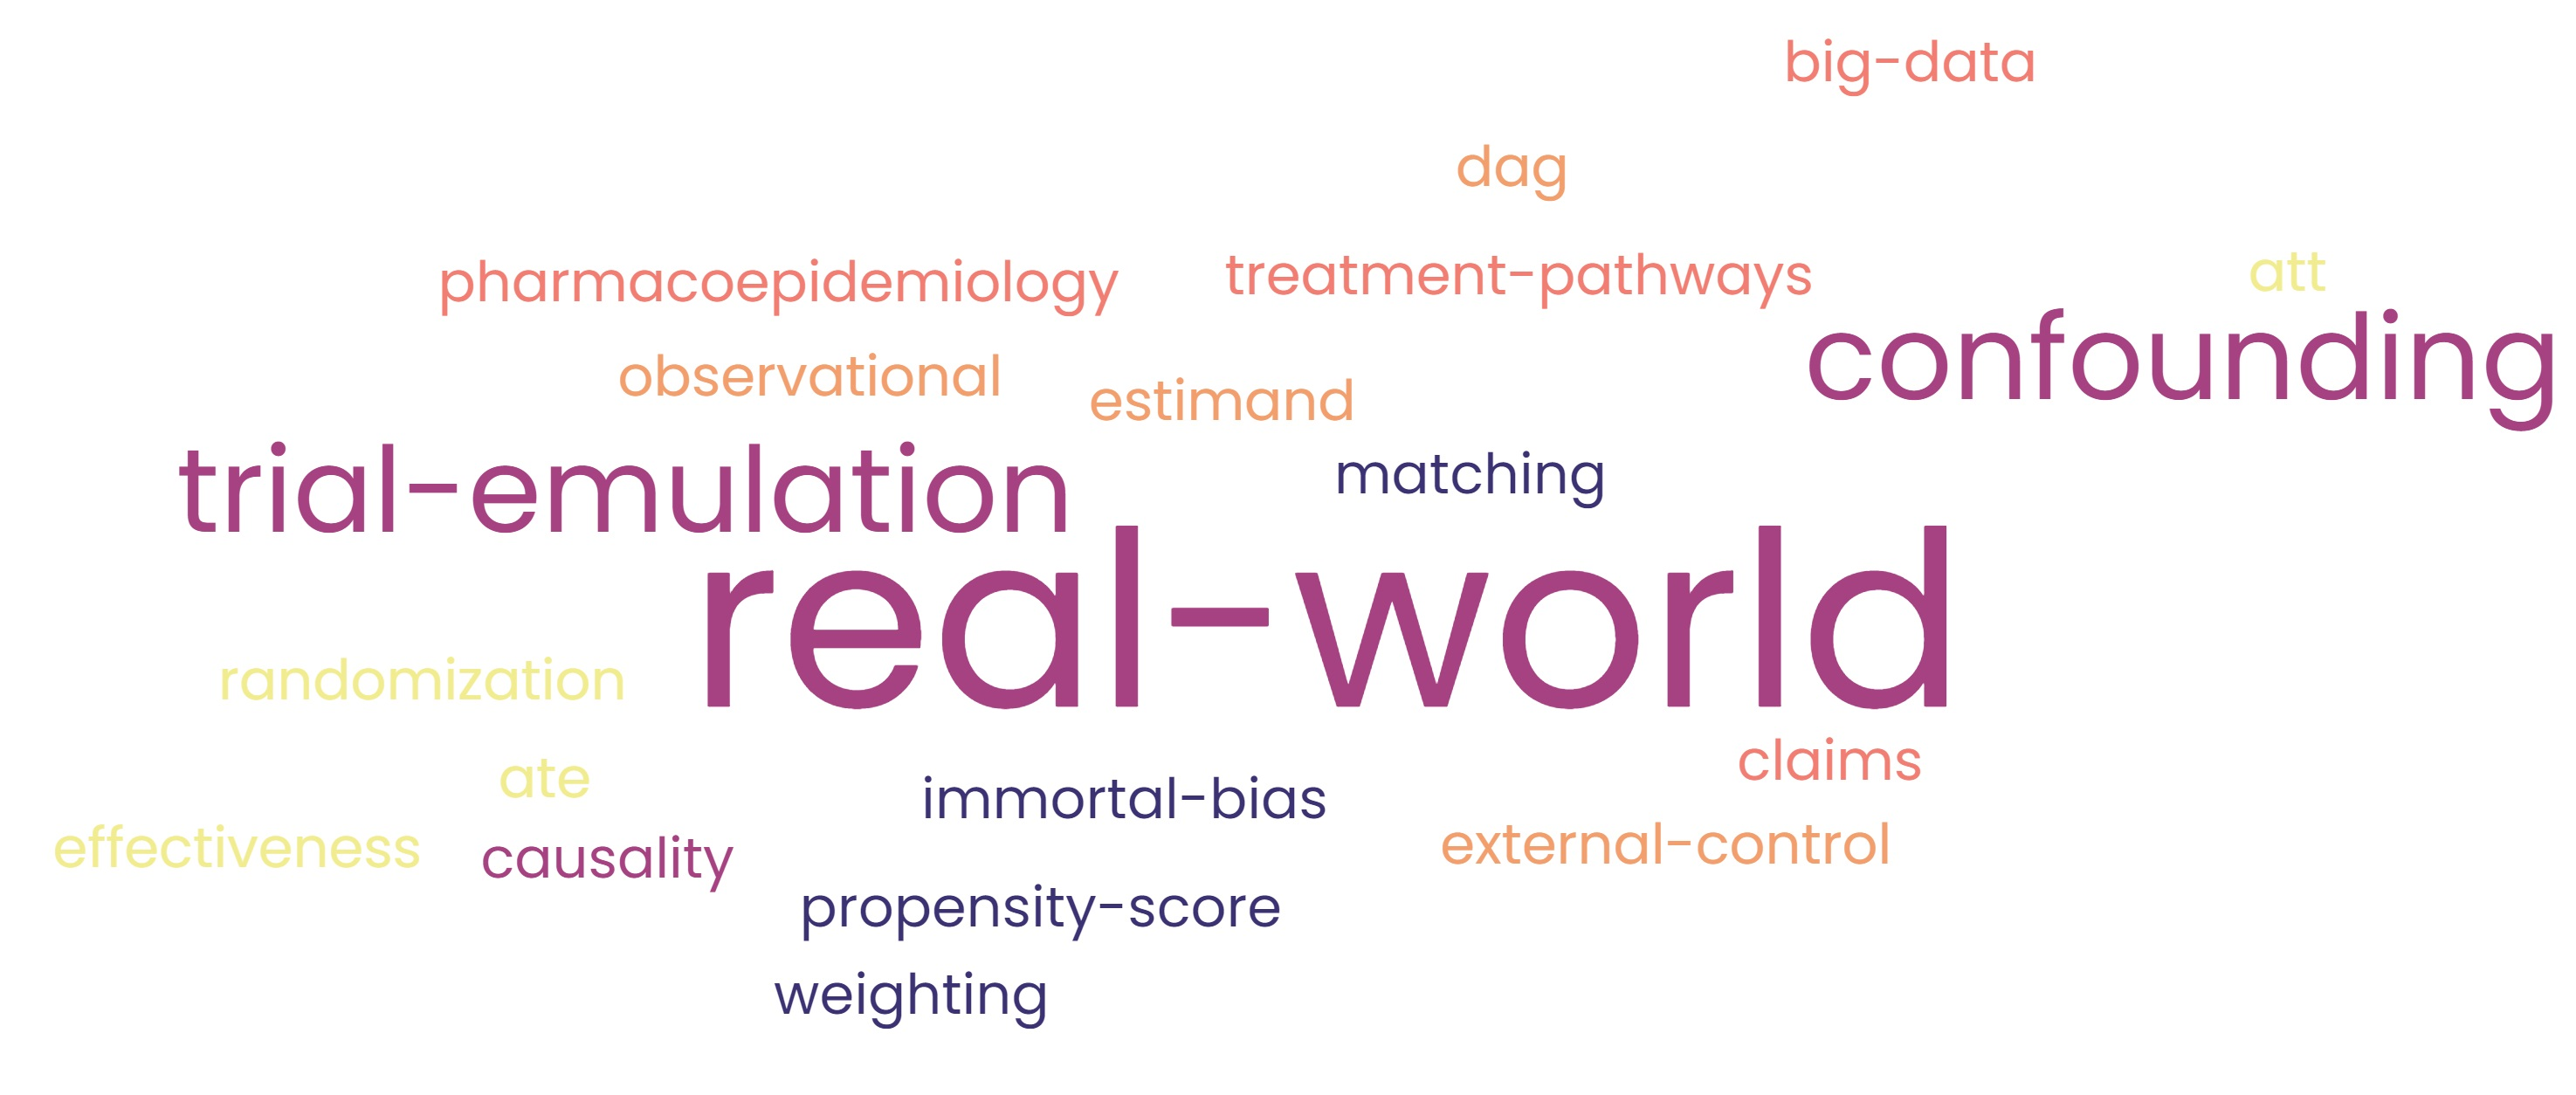
\includegraphics[width=0.8\linewidth]{images/cloudword} \end{center}

This book begins with \textbf{Chapter} @ref(introduction), which offers
an overview of RWD, highlighting key concepts and the challenges
commonly encountered in this field.

Following this, a motivating example is introduced in \textbf{Chapter}
@ref(motivating-example), which will be used throughout the book to
illustrate each subsequent chapter with practical R code for
reproducibility (used packages are listed in Appendix @ref(r-packages)).

The next chapters focus on approaches to limit these inherent biases:

\begin{itemize}
\item
  \textbf{Chapter} @ref(target-trial-emulation) presents the Hernán et
  al.~framework, a key approach to Target Trial Emulation (TTE) that
  strengthens the reliability of Real World Evidence (RWE) to address
  inherent biases.
\item
  \textbf{Chapter} @ref(iptw-application) focuses on Propensity Score
  (PS) techniques aiming to reduce confounding bias at baseline.
\item
  \textbf{Chapter} @ref(clone-censor-weight) examines the
  Clone-Censor-Weight (CCW) approach, a method to limit both confounding
  and immortal bias in the context of time-varying treatments.
\end{itemize}

\chapter*{About the author}\label{author}
\addcontentsline{toc}{chapter}{About the author}

\textbf{Quentin Pilard
(\href{mailto:pilard.quentin@gmail.com}{\nolinkurl{pilard.quentin@gmail.com}})}

This tutorial is based on my four years of experience at Quinten Health
(Paris) working with RWD in collaboration with pharmaceutical industries
and academia

\begin{center}
\includegraphics[width=0.3\linewidth]{images/moi} \end{center}

\chapter{Introduction}\label{introduction}

\section{Definition}\label{definition}

According to the main regulatory agencies, these are the definition of
\textbf{RWD} and \textbf{RWE}
(\citeproc{ref-baumfeld_andre_trial_2020}{Baumfeld Andre et al. 2020}):

\begin{longtable}[]{@{}
  >{\centering\arraybackslash}p{(\columnwidth - 4\tabcolsep) * \real{0.3333}}
  >{\centering\arraybackslash}p{(\columnwidth - 4\tabcolsep) * \real{0.3333}}
  >{\centering\arraybackslash}p{(\columnwidth - 4\tabcolsep) * \real{0.3333}}@{}}
\toprule\noalign{}
\begin{minipage}[b]{\linewidth}\centering
Regulatory agency
\end{minipage} & \begin{minipage}[b]{\linewidth}\centering
Real-World Data
\end{minipage} & \begin{minipage}[b]{\linewidth}\centering
Real-World Evidence
\end{minipage} \\
\midrule\noalign{}
\endhead
\bottomrule\noalign{}
\endlastfoot
FDA (USA) & Data relating to patient health status and/or the delivery
of health care routinely collected from a variety of sources & Clinical
evidence about the usage and potential benefits or risks of a medical
product derived from analysis of RWD \\
EMA (Europe) & Health care related data that is collected outside of
randomized clinical trials & Evidence coming from registries, electronic
health records, and insurance data \\
PMDA (Japan) & Utilization of patient registry data and medical
information database & No definition was found \\
\end{longtable}

As presented, definitions are fairly consistent with each other.

\section{Use of RWD in drug
development}\label{use-of-rwd-in-drug-development}

In drug development, RWD has traditionally been used in post-market
safety surveillance. However, its potential applications extend
throughout the entire drug lifecycle
(\citeproc{ref-khosla_real_2018}{Khosla et al. 2018}). This includes:

\begin{enumerate}
\def\labelenumi{\arabic{enumi}.}
\item
  \textbf{Discovery and Early Development:}

  \emph{Purpose}: Characterize disease epidemiology and unmet needs.

  \emph{RWE Use}: Helps define the target product profile by analyzing
  disease burden and patient characteristics, guiding the selection of
  indications and prioritizing development.
\item
  \textbf{Phase 1--3 Clinical Trials:}

  \emph{Purpose:} Design clinical trials and ensure they reflect
  real-world populations.

  \emph{RWE Use}: Provides insights into real-world patient populations
  and treatment patterns, helping to refine inclusion/exclusion criteria
  and improve the external validity of trials.
\item
  \textbf{Regulatory Approval:}

  \emph{Purpose:} Obtain marketing authorization for new drugs.

  \emph{RWE Use}: Supports clinical trial data by providing additional
  evidence on real-world safety, efficacy, and patient outcomes,
  potentially accelerating approval processes.
\item
  \textbf{Post-Approval (Phase 4) and Market Access:}

  \emph{Purpose:} Ensure broad access and reimbursement.

  \emph{RWE Use:} Provides evidence on the real-world effectiveness,
  safety, and cost-effectiveness of the drug compared to standard care,
  supporting reimbursement decisions and market access strategies.
\item
  \textbf{Post-Market Surveillance and Lifecycle Management:}

  \emph{Purpose:} Monitor long-term safety and maintain market access.

  \emph{RWE Use:} Continuously tracks patient outcomes, adherence, and
  safety data in real-world settings, supporting the long-term value
  demonstration and label expansion into new populations or indications.
\end{enumerate}

\section{Regulators acceptance of
RWD}\label{regulators-acceptance-of-rwd}

RWD is gaining increasing interest and acceptance from regulators as a
\textbf{complement to clinical trial} findings. For example, various
frameworks have been established, such as the ``\textbf{Real-World
Evidence Framework to Support EU Regulatory Decision-Making}'' by the
EMA and the ``\textbf{Real-World Evidence Program}'' by the FDA
(\citeproc{ref-ema_2024}{EMA 2023};
\citeproc{ref-fda_real-world_2024}{FDA 2018}). Additionally, the FDA has
issued guidance for industry titled ``\textbf{Considerations for the Use
of Real-World Data and Real-World Evidence to Support Regulatory
Decision-Making for Drug and Biological Products}''
(\citeproc{ref-fda_considerations}{FDA 2023}).

Moreover, FDA-funded initiative like the \textbf{DUPLICATE} program have
been undertaken. This program focuses on replicating large-scale
Randomized Controlled Trials (RCTs) using RWD to evaluate the
reliability and confidence in analyses based on RWD
(\citeproc{ref-franklin_emulating_2021}{Franklin et al. 2021}).

\section{Use of External Control Arm and Target Trial
Emulation}\label{use-of-external-control-arm-and-target-trial-emulation}

While RCTs remain the gold standard for generating unbiased evidence due
to their controlled and randomized nature, there are situations where a
traditional control group is not available or feasible. In such cases,
researchers can resort to two alternative approaches: \textbf{External
Control Arm (ECA)} or the \textbf{Target Trial Emulation (TTE)}
(\citeproc{ref-baumfeld_andre_trial_2020}{Baumfeld Andre et al. 2020};
\citeproc{ref-hernan_using_2016}{Hernán and Robins 2016}). These two
methods are illustrated below:

\begin{figure}

{\centering \includegraphics[width=0.8\linewidth]{images/Présentation3} 

}

\caption{Main study designs using RWD}\label{fig:unnamed-chunk-3}
\end{figure}

The ECA method involves using historical or real-world data as a
comparative baseline, offering a way to evaluate the effectiveness of a
treatment in the absence of a control group. Alternatively, the TTE
seeks to replicate the design of an RCT as closely as possible, but
within the context of RWD.

\section{Main biases in RWD}\label{main-biases-in-rwd}

Although RWD is a viable alternative to RCT, it comes, as any
observational studies, with inherent bias due to the lack of
randomization (\citeproc{ref-encepp_2010}{ENCePP 2010}). These are the
most common:

\begin{itemize}
\item
  \textbf{Selection bias}: Arises from the non-random selection of
  treatment groups.
\item
  \textbf{Information bias}: Results from inaccuracies in data
  collection.
\item
  \textbf{Confounding bias}: Occurs when external factors distort the
  association between the treatment and the outcome.
\item
  \textbf{Immortal time bias}: Happens during a follow-up period when
  the event of interest, often death, cannot occur.
\end{itemize}

\chapter{Motivating example}\label{motivating-example}

Persistent Depressive Disorder (PDD) is a chronic mood disorder
characterized by a consistently low mood that lasts for at least two
years, significantly impacting patients' quality of life.

\begin{center}
\includegraphics[width=0.5\linewidth]{images/PDD} \end{center}

Antidepressants serve as the primary treatment for PDD, aiding in
symptom management and reducing the risk of relapse. Among these
medications, Sertralex and Duloxyn are frequently prescribed, each
operating through distinct mechanisms.

This study aims to compare the effectiveness of Sertralex and Duloxyn in
prolonging the time to relapse over a maximum follow-up period of one
year, representing the typical treatment duration for patients newly
diagnosed with PDD.

To capture different clinical settings, we consider two scenarios:

\begin{itemize}
\item
  \textbf{Scenario 1:} In this simplified setup, treatment with
  Sertralex or Duloxyn begins immediately following the PDD diagnosis.
\item
  \textbf{Scenario 2:} In a more realistic setup, a 30-day ``grace
  period'' is introduced---a period following PDD diagnosis during which
  treatment initiation can occur. This grace period reflects common
  clinical practice, as clinicians may not always recommend immediate
  drug therapy after diagnosis.
\end{itemize}

Here is the list of variables included in the dataset:

\begin{itemize}
\item
  \textbf{ID}: Patient identifier
\item
  \textbf{AGE}: Age at diagnosis (years)
\item
  \textbf{GENDER}: Gender of the patient {[}0=Male; 1=Female{]}
\item
  \textbf{BECK}: Beck Depression Inventory score at diagnosis {[}0 (best
  prognosis) - 63 (worst prognosis){]}
\item
  \textbf{SOCIO\_ECO}: Socioeconomic status {[}1=Very low; 2=Low;
  3=Moderate; 4=High; 5=Very high{]}
\item
  \textbf{EVENT}: Relapse indicator {[}0=No relapse; 1=Relapse{]}
\item
  \textbf{TIME\_TO\_EVENT}: Time from diagnosis to event of interest or
  censoring (in days)
\item
  \textbf{TREAT}: Therapy initiated at diagnosis {[}0=Sertralex;
  1=Duloxyn{]}.
\item
  \textbf{TIME\_TO\_TREAT}: Time from diagnosis to treatment (in days)
\end{itemize}

Further information on the simulation process to generate these data are
described in Appendix @ref(r-code).

\chapter{Target Trial Emulation using observational
data}\label{target-trial-emulation}

\section{Background}\label{background}

In 2016, Hernán and Rubins presented a framework to emulate a clinical
trial using observational data when no clinical trial exists
(\citeproc{ref-hernan_using_2016}{Hernán and Robins 2016}).The latter is
a 2-step process: (1) \textbf{Specifying the target trial} (i.e., which
is the hypothetical trial that could have been performed to answer the
research question). This includes these elements eligibility criteria,
treatment strategies, assignment procedures, follow-up period, outcome,
causal contrast of interest and analysis plan, and (2) \textbf{Emulating
each element} from the target trial.

Let us illustrate the TTE framework using our motivating example.

\section{Specify the target trial}\label{specify-the-target-trial}

As suggested, we specified the target trial as below:

\begin{longtable}[]{@{}
  >{\raggedright\arraybackslash}p{(\columnwidth - 4\tabcolsep) * \real{0.1535}}
  >{\raggedright\arraybackslash}p{(\columnwidth - 4\tabcolsep) * \real{0.8377}}
  >{\raggedright\arraybackslash}p{(\columnwidth - 4\tabcolsep) * \real{0.0044}}@{}}
\toprule\noalign{}
\begin{minipage}[b]{\linewidth}\raggedright
Protocol component
\end{minipage} & \begin{minipage}[b]{\linewidth}\raggedright
Target trial emulation
\end{minipage} & \begin{minipage}[b]{\linewidth}\raggedright
\end{minipage} \\
\midrule\noalign{}
\endhead
\bottomrule\noalign{}
\endlastfoot
\textbf{Eligibility criteria} & Individuals aged 18 or older, newly
diagnosed with PDD. & \\
\textbf{Treatment strategies} & Individuals who initiated Sertralex or
Duloxyn. & \\
\textbf{Assignment procedures} & Individuals randomly assigned to either
strategy at baseline and are not aware of the assigned strategy & \\
\textbf{Follow-up period} & Starts at randomization and ends at the
first occurrence of a relapse event, death, or after one year of
follow-up, whichever occurs first. & \\
\textbf{Outcome} & Relapse (defined as a recurrence of depressive
disorder) diagnosed by a clinician, identified through clinical
assessment or documented diagnosis of depression during the follow-up
period. & \\
\textbf{Causal contrasts of interest} & Intention-to-treat (ITT): Effect
of being assigned to treatment strategies at randomization, regardless
of whether individuals adhere to them during follow-up.

Per Protocol (PP): Individuals who discontinued treatment during
follow-up were right censored at the first occurence.

(see Appendix @ref(ich) for causal contrasts of interest defined as
formulated in the ICH E9 (R1) addendum) & \\
\textbf{Analysis plan} &
\multicolumn{2}{>{\raggedright\arraybackslash}p{(\columnwidth - 4\tabcolsep) * \real{0.8421} + 2\tabcolsep}@{}}{%
In both analyses (ITT and PP), Kaplan-Meier estimates and Cox
proportional hazards models were utilized to compare the time to relapse
from randomization between Sertralex and Duloxyn \textbar{} \textbar{}
To estimate the validity of PP, adjustment for post randomization
confunding is anticipated using Inverse Probability of Censoring
Weighted (IPCW) methods (\citeproc{ref-robins_correcting_2000}{Robins
and Finkelstein 2000})} \\
\end{longtable}

\section{Emulate the target trial}\label{emulate-the-target-trial}

Next, we examined each component and detailed how they can be derived
using RWD.

\textbf{Eligibility criteria}: We included individuals aged 18 or older
who were firstly diagnosed with PDD.

\textbf{Treatment strategies}: We defined two treatment strategies:
either Sertralex or Duloxyn as the first prescription following a PDD
diagnosis. In scenario 1 (see Chapter @ref(motivating-example)), this is
considered as immediate, while in scenario 2, we allowed a period of up
to 30 days to record the first initiation.

\textbf{Assignment procedures}: We assumed these two groups were
exchangeable at the date of PDD diagnosis (or up to 30 days following
PDD diagnosis for scenario 2), conditionally on baseline covariates:
Age, gender, Beck score and socioeconomic status.

\textbf{Follow-up periods}: We defined time zero as the date of PDD
diagnosis. From this point, we followed-up individuals until the
earliest of the following events: first clinical relapse, loss of
follow-up (corresponds to the last activity record in the database), 365
days after time zero.

\textbf{Outcomes}: We assumed the outcome as the first relapse occurring
after time zero.

\textbf{Causal contrast of interest}: We considered observational
analogues of the ITT and PP effect. However, the ITT effect in the
emulated trial is closer to a PP effect, as we lack information on
treatment discontinuation, and thus assumed full adherence throughout
the study.

\textbf{Analysis plan}: In scenario 1, we used Inverse Probability
Treatment Weights (IPTW) to emulate the randomization process and
applied these weights in the outcome analysis, including weighted
Kaplan-Meier estimates and Cox proportional hazards models (see Chapter
@ref(iptw-application) for further details). In scenario 2, we
implemented the Clone-Censor-Weight method (CCW) to address both
confounding and immortal time bias due to the permitted delay between
PDD diagnosis and treatment initiation (see Chapter
@ref(clone-censor-weight) for further details).

\chapter{Propensity score methods}\label{iptw-application}

\section{Background}\label{background-1}

The \textbf{Propensity Score (PS)} is utilized to emulate the
randomization process, with the goal of balancing the population's
characteristics across the groups of interest. Unlike multivariable
regression, which focuses on estimating the effect at the individual
level (\emph{subject-specific effect}), the PS method estimates the
effect at the population level (\emph{population-average effect}). In
the context of models with a non-linear link (typically when Odds Ratio
{[}OR{]} or Hazard Ratio {[}HR{]} are reported), these two effects
differ (\citeproc{ref-austin_conditioning_2007}{Austin et al. 2007}).

Statistically, the PS is defined as the conditional probability of
receiving the exposure of interest based on observed baseline
characteristics. It is typically estimated using multivariable logistic
regression, where the exposure of interest serves as the dependent
variable and the baseline characteristics act as independent variables.
Once calculated, it can be employed in various approaches, including
matching, stratification, \textbf{Inverse Probability of Treatment
Weighting} (IPTW), and covariate adjustment
(\citeproc{ref-austin_introduction_2011}{Austin 2011}).

The scenario 1 discussed in Chapter @ref(motivating-example) will be
applied to illustrate the application of IPTW.

\section{Identify confounders}\label{identify-confounders}

The baseline characteristics incorporated in the logistic regression
must be defined as \textbf{confounders - variables that influence both
treatment assignment and the outcome without being part on the causal
pathway}. Other types of variables, such as \textbf{mediators or
colliders}, may also be present; however, adjusting for these can
introduce bias (\citeproc{ref-mackinnon_unification_2021}{MacKinnon and
Lamp 2021}).

\textbf{Directed Acyclic Graphs} (DAGs) are usually recommended to
depict causal relationships, ideally, clinical experts should be
involved in their development as they more likely to know involved
clinical pathways, interacting with the disease of interest
(\citeproc{ref-hernan_causal_nodate}{Hernan and Robins 2024};
\citeproc{ref-tennant_use_2021}{Tennant et al. 2021}). DAGs can be
created using the DAGitty \href{https://www.dagitty.net/}{website} or
dagitty R \href{https://github.com/jtextor/dagitty}{package}.

In our example, we identified age at diagnosis, gender, Beck score and
socioeconomic status as potential confounders of the association between
treatment exposure and relapse. The associated DAG is represented in
Appendix @ref(dag).

\section{IPTW implementation}\label{iptw-implementation}

This code implements the IPTW approach using the \textbf{stabilized
Average Treatment Effect (ATE)} estimand
(\citeproc{ref-austin_moving_2015}{Austin and Stuart 2015}), detailed in
the following equation:

\[
IPTW_{Stabilized, ATE} = \frac{X*Pr(X=1)}{e}+\frac{(1-X)*Pr(X=0)}{1-e} 
\]

Here, the PS is defined as \(e = \Pr ({X}=1|{Z}={z})\) and \(X\) and
\(Z\) are the treatment status (0 = Sertralex and 1 = Duloxyn) and
observed confunders (gender, age, SES level, and Beck score),
respectively.

This models the treatment effect across the entire population likely to
receive either Sertralex or Duloxyn. Additional details on causal
estimands (ATE/ATT) are provided in Appendix @ref(causal).

\begin{Shaded}
\begin{Highlighting}[]
\CommentTok{\#Perform weighting}
\NormalTok{W }\OtherTok{\textless{}{-}}\NormalTok{ WeightIt}\SpecialCharTok{::}\FunctionTok{weightit}\NormalTok{(TREAT }\SpecialCharTok{\textasciitilde{}}\NormalTok{ AGE }\SpecialCharTok{+}\NormalTok{ GENDER }\SpecialCharTok{+}\NormalTok{ SOCIO\_ECO }\SpecialCharTok{+}\NormalTok{ BECK,}
                            \AttributeTok{data =}\NormalTok{ data,}
                            \AttributeTok{method =} \StringTok{"glm"}\NormalTok{,}
                            \AttributeTok{estimand =} \StringTok{"ATE"}\NormalTok{,}
                            \AttributeTok{stabilize =} \ConstantTok{TRUE}\NormalTok{)}
\NormalTok{data}\SpecialCharTok{$}\NormalTok{weights }\OtherTok{\textless{}{-}}\NormalTok{ W}\SpecialCharTok{$}\NormalTok{weights}
\NormalTok{data}\SpecialCharTok{$}\NormalTok{ps }\OtherTok{\textless{}{-}}\NormalTok{ W}\SpecialCharTok{$}\NormalTok{ps}
\end{Highlighting}
\end{Shaded}

\section{Balance Diagnostics}\label{balance-diagnostics}

To evaluate balance after weighting, we applied the typical
recommendation by using the Standardized Mean Difference (SMD) and
checking whether the difference in SMD is less than 0.1
(\citeproc{ref-austin_balance_2009}{Austin 2009};
\citeproc{ref-normand_validating_2001}{Normand et al. 2001}). A
difference below this threshold indicates that the characteristics of
interest are balanced between the groups.

\begin{Shaded}
\begin{Highlighting}[]
\FunctionTok{love.plot}\NormalTok{(W, }
          \AttributeTok{binary =} \StringTok{"std"}\NormalTok{, }
          \AttributeTok{thresholds =} \FunctionTok{c}\NormalTok{(}\AttributeTok{m =}\NormalTok{ .}\DecValTok{1}\NormalTok{),}
          \AttributeTok{sample.names =} \FunctionTok{c}\NormalTok{(}\StringTok{"Before weighting"}\NormalTok{, }\StringTok{"After weighting"}\NormalTok{))}
\end{Highlighting}
\end{Shaded}

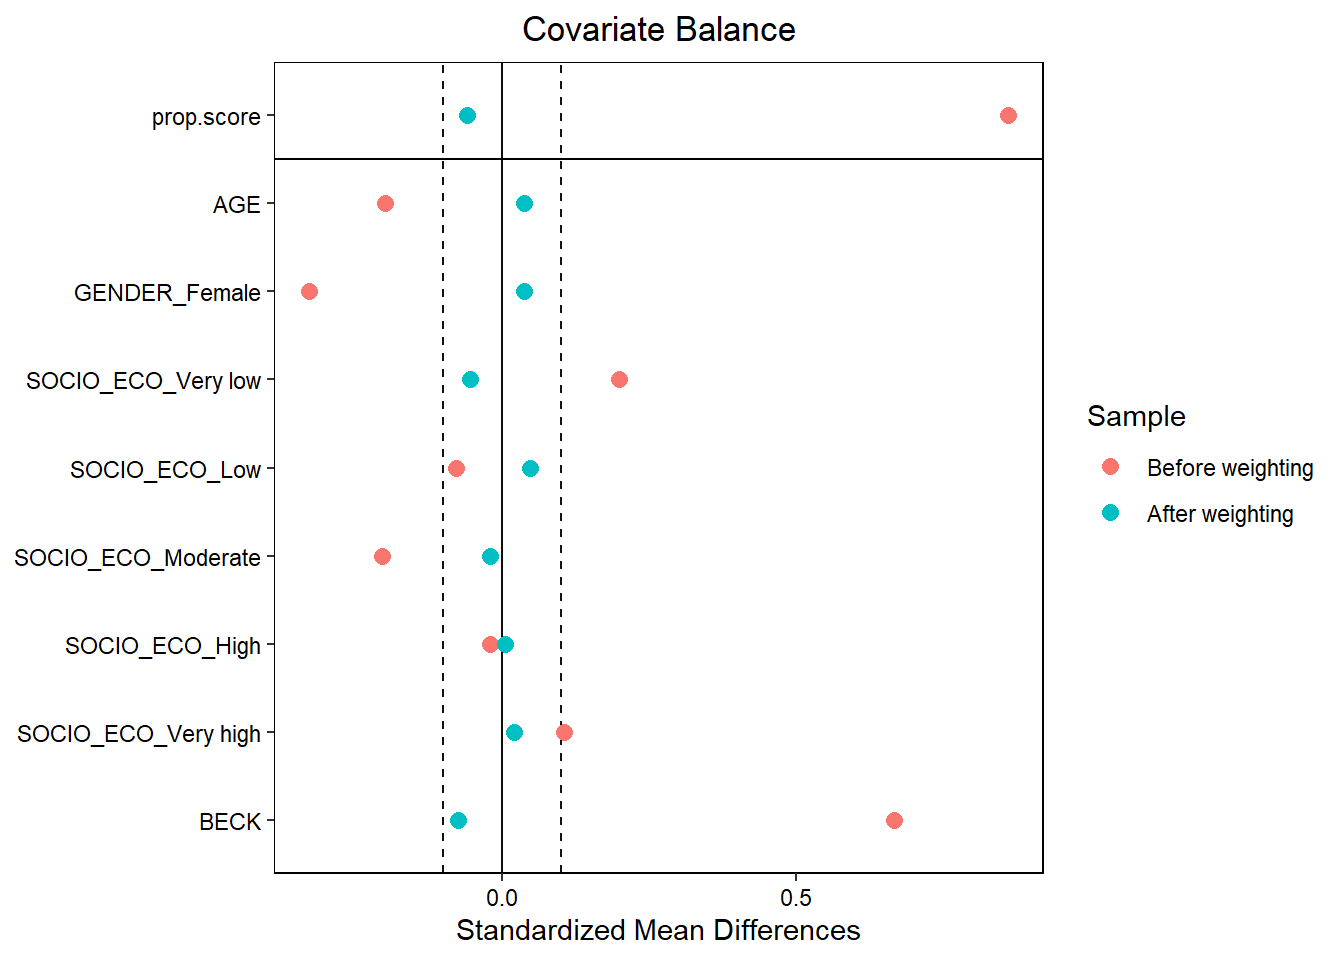
\includegraphics{_main_files/figure-latex/love_plot-1.pdf}

To summarize, a table before and after weighting is also represented
according to treatment status.

\begin{Shaded}
\begin{Highlighting}[]
\CommentTok{\#Before weighting}
\NormalTok{t1 }\OtherTok{\textless{}{-}}\NormalTok{ data }\SpecialCharTok{\%\textgreater{}\%}
  \FunctionTok{select}\NormalTok{(AGE, GENDER, SOCIO\_ECO, BECK, TREAT) }\SpecialCharTok{\%\textgreater{}\%}
  \FunctionTok{tbl\_summary}\NormalTok{(}\AttributeTok{by =}\NormalTok{ TREAT, }
              \AttributeTok{statistic =} \FunctionTok{list}\NormalTok{(}\FunctionTok{all\_continuous}\NormalTok{() }\SpecialCharTok{\textasciitilde{}} \StringTok{"\{mean\} (\{sd\})"}\NormalTok{),}
              \AttributeTok{label =} \FunctionTok{list}\NormalTok{(AGE }\SpecialCharTok{\textasciitilde{}} \StringTok{"Age (at diagnosis)"}\NormalTok{,}
\NormalTok{                           GENDER }\SpecialCharTok{\textasciitilde{}} \StringTok{"Gender"}\NormalTok{,}
\NormalTok{                           SOCIO\_ECO }\SpecialCharTok{\textasciitilde{}} \StringTok{"SES level (1{-}5)"}\NormalTok{,}
\NormalTok{                           BECK }\SpecialCharTok{\textasciitilde{}} \StringTok{"Beck score (0{-}63)"}\NormalTok{),}
              \AttributeTok{digits =} \FunctionTok{all\_continuous}\NormalTok{() }\SpecialCharTok{\textasciitilde{}} \DecValTok{1}\NormalTok{) }\SpecialCharTok{\%\textgreater{}\%}
  \FunctionTok{add\_difference}\NormalTok{(}\AttributeTok{test =} \FunctionTok{everything}\NormalTok{() }\SpecialCharTok{\textasciitilde{}} \StringTok{"smd"}\NormalTok{) }\SpecialCharTok{\%\textgreater{}\%}
  \FunctionTok{modify\_header}\NormalTok{(label }\SpecialCharTok{\textasciitilde{}} \StringTok{"**Variable**"}\NormalTok{, }
\NormalTok{                estimate }\SpecialCharTok{\textasciitilde{}} \StringTok{"**SMD**"}\NormalTok{, }
\NormalTok{                stat\_1 }\SpecialCharTok{\textasciitilde{}} \FunctionTok{paste0}\NormalTok{(}\StringTok{"**Sertralex (N="}\NormalTok{,}\FunctionTok{nrow}\NormalTok{(data[}\FunctionTok{which}\NormalTok{(data}\SpecialCharTok{$}\NormalTok{TREAT}\SpecialCharTok{==}\StringTok{"Sertralex"}\NormalTok{),]),}\StringTok{")**"}\NormalTok{), }
\NormalTok{                stat\_2 }\SpecialCharTok{\textasciitilde{}} \FunctionTok{paste0}\NormalTok{(}\StringTok{"**Duloxyn (N="}\NormalTok{,}\FunctionTok{nrow}\NormalTok{(data[}\FunctionTok{which}\NormalTok{(data}\SpecialCharTok{$}\NormalTok{TREAT}\SpecialCharTok{==}\StringTok{"Duloxyn"}\NormalTok{),]),}\StringTok{")**"}\NormalTok{))}
\NormalTok{data\_selected }\OtherTok{\textless{}{-}}\NormalTok{ data }\SpecialCharTok{\%\textgreater{}\%}
  \FunctionTok{select}\NormalTok{(AGE, GENDER, SOCIO\_ECO, BECK, TREAT)}

\CommentTok{\#After weighting}
\NormalTok{data\_svy }\OtherTok{\textless{}{-}} \FunctionTok{svydesign}\NormalTok{(}\AttributeTok{ids =} \SpecialCharTok{\textasciitilde{}}\DecValTok{1}\NormalTok{, }\AttributeTok{data =}\NormalTok{ data\_selected, }\AttributeTok{weights =} \SpecialCharTok{\textasciitilde{}}\NormalTok{W}\SpecialCharTok{$}\NormalTok{weights)}
\NormalTok{t2 }\OtherTok{\textless{}{-}}\NormalTok{ data\_svy }\SpecialCharTok{\%\textgreater{}\%}
  \FunctionTok{tbl\_svysummary}\NormalTok{(}\AttributeTok{by =}\NormalTok{ TREAT, }
                 \AttributeTok{statistic =} \FunctionTok{list}\NormalTok{(}\FunctionTok{all\_continuous}\NormalTok{() }\SpecialCharTok{\textasciitilde{}} \StringTok{"\{mean\} (\{sd\})"}\NormalTok{),}
                 \AttributeTok{label =} \FunctionTok{list}\NormalTok{(AGE }\SpecialCharTok{\textasciitilde{}} \StringTok{"Age (at diagnosis)"}\NormalTok{,}
\NormalTok{                           GENDER }\SpecialCharTok{\textasciitilde{}} \StringTok{"Gender"}\NormalTok{,}
\NormalTok{                           SOCIO\_ECO }\SpecialCharTok{\textasciitilde{}} \StringTok{"SES level (1{-}5)"}\NormalTok{,}
\NormalTok{                           BECK }\SpecialCharTok{\textasciitilde{}} \StringTok{"Beck score (0{-}63)"}\NormalTok{),}
                 \AttributeTok{digits =} \FunctionTok{all\_continuous}\NormalTok{() }\SpecialCharTok{\textasciitilde{}} \DecValTok{1}\NormalTok{) }\SpecialCharTok{\%\textgreater{}\%}
  \FunctionTok{add\_difference}\NormalTok{(}\AttributeTok{test =} \FunctionTok{everything}\NormalTok{() }\SpecialCharTok{\textasciitilde{}} \StringTok{"smd"}\NormalTok{) }\SpecialCharTok{\%\textgreater{}\%}
  \FunctionTok{modify\_header}\NormalTok{(label }\SpecialCharTok{\textasciitilde{}} \StringTok{"**Variable**"}\NormalTok{, }
\NormalTok{                estimate }\SpecialCharTok{\textasciitilde{}} \StringTok{"**SMD**"}\NormalTok{, }
\NormalTok{                stat\_1 }\SpecialCharTok{\textasciitilde{}} \FunctionTok{paste0}\NormalTok{(}\StringTok{"**Sertralex (N="}\NormalTok{,}\FunctionTok{round}\NormalTok{(}\FunctionTok{ESS}\NormalTok{(W}\SpecialCharTok{$}\NormalTok{weights[W}\SpecialCharTok{$}\NormalTok{treat}\SpecialCharTok{==}\StringTok{"Sertralex"}\NormalTok{]),}\DecValTok{0}\NormalTok{),}\StringTok{")**"}\NormalTok{), }
\NormalTok{                stat\_2 }\SpecialCharTok{\textasciitilde{}} \FunctionTok{paste0}\NormalTok{(}\StringTok{"**Duloxyn (N="}\NormalTok{,}\FunctionTok{round}\NormalTok{(}\FunctionTok{ESS}\NormalTok{(W}\SpecialCharTok{$}\NormalTok{weights[W}\SpecialCharTok{$}\NormalTok{treat}\SpecialCharTok{==}\StringTok{"Duloxyn"}\NormalTok{]),}\DecValTok{0}\NormalTok{),}\StringTok{")**"}\NormalTok{)) }

\ControlFlowTok{for}\NormalTok{ (int\_col }\ControlFlowTok{in} \FunctionTok{c}\NormalTok{(}\StringTok{"modify\_stat\_N"}\NormalTok{, }\StringTok{"modify\_stat\_n"}\NormalTok{)) \{}
\NormalTok{  t1}\SpecialCharTok{$}\NormalTok{table\_styling}\SpecialCharTok{$}\NormalTok{header[[int\_col]] }\OtherTok{\textless{}{-}}
\NormalTok{    t1}\SpecialCharTok{$}\NormalTok{table\_styling}\SpecialCharTok{$}\NormalTok{header[[int\_col]] }\SpecialCharTok{|\textgreater{}} \FunctionTok{as.numeric}\NormalTok{()}
\NormalTok{\}}

\FunctionTok{tbl\_merge}\NormalTok{(}\AttributeTok{tbls =} \FunctionTok{list}\NormalTok{(t1, t2),}
          \AttributeTok{tab\_spanner =} \FunctionTok{c}\NormalTok{(}
            \FunctionTok{paste0}\NormalTok{(}\StringTok{"**Raw (N="}\NormalTok{,}\FunctionTok{nrow}\NormalTok{(data),}\StringTok{")**"}\NormalTok{), }
            \FunctionTok{paste0}\NormalTok{(}\StringTok{"**Weighted (ESS="}\NormalTok{,}\FunctionTok{round}\NormalTok{(}\FunctionTok{ESS}\NormalTok{(W}\SpecialCharTok{$}\NormalTok{weights),}\DecValTok{0}\NormalTok{),}\StringTok{")**"}\NormalTok{)}
\NormalTok{            )}
\NormalTok{          )}\SpecialCharTok{\%\textgreater{}\%}
  \FunctionTok{modify\_table\_body}\NormalTok{(}\SpecialCharTok{\textasciitilde{}}\NormalTok{ .x }\SpecialCharTok{\%\textgreater{}\%} \FunctionTok{select}\NormalTok{(}\SpecialCharTok{{-}}\NormalTok{conf.low\_1, }\SpecialCharTok{{-}}\NormalTok{conf.low\_2))}
\end{Highlighting}
\end{Shaded}

\begin{table}[!t]
\fontsize{12.0pt}{14.4pt}\selectfont
\begin{tabular*}{\linewidth}{@{\extracolsep{\fill}}lcccccc}
\toprule
 & \multicolumn{3}{c}{\textbf{Raw (N=508)}} & \multicolumn{3}{c}{\textbf{Weighted (ESS=468)}} \\ 
\cmidrule(lr){2-4} \cmidrule(lr){5-7}
\textbf{Variable} & \textbf{Sertralex (N=299)}\textsuperscript{\textit{1}} & \textbf{Duloxyn (N=209)}\textsuperscript{\textit{1}} & \textbf{SMD}\textsuperscript{\textit{2}} & \textbf{Sertralex (N=281)}\textsuperscript{\textit{1}} & \textbf{Duloxyn (N=188)}\textsuperscript{\textit{1}} & \textbf{SMD}\textsuperscript{\textit{2}} \\ 
\midrule\addlinespace[2.5pt]
Age (at diagnosis) & 32.5 (6.0) & 31.9 (5.7) & 0.12 & 32.1 (6.2) & 32.0 (5.7) & 0.01 \\ 
Gender &  &  & 0.32 &  &  & 0.00 \\ 
    Male & 142 (47\%) & 132 (63\%) &  & 164 (54\%) & 113 (55\%) &  \\ 
    Female & 157 (53\%) & 77 (37\%) &  & 137 (46\%) & 94 (45\%) &  \\ 
SES level (1-5) &  &  & 0.24 &  &  & 0.02 \\ 
    Very low & 59 (20\%) & 47 (22\%) &  & 66 (22\%) & 46 (22\%) &  \\ 
    Low & 58 (19\%) & 35 (17\%) &  & 55 (18\%) & 39 (19\%) &  \\ 
    Moderate & 67 (22\%) & 32 (15\%) &  & 59 (19\%) & 39 (19\%) &  \\ 
    High & 62 (21\%) & 44 (21\%) &  & 61 (20\%) & 40 (19\%) &  \\ 
    Very high & 53 (18\%) & 51 (24\%) &  & 61 (20\%) & 42 (20\%) &  \\ 
Beck score (0-63) & 25.3 (7.5) & 27.8 (6.4) & -0.37 & 26.5 (7.5) & 26.6 (6.9) & -0.01 \\ 
\bottomrule
\end{tabular*}
\begin{minipage}{\linewidth}
\textsuperscript{\textit{1}}Mean (SD); n (\%)\\
\textsuperscript{\textit{2}}Standardized Mean Difference\\
\end{minipage}
\end{table}

After weighting, observed confunders were above the recommended
threshold. If, after weighting, the observed confounders exceed the
recommended threshold, the model can be respecified (e.g.~making a
continuous variable categorical or dichotomous, including higher order
terms or splines of variables, \ldots). Otherwise, variables with
remaining imbalance should ideally be adjusted for when modeling the
final outcome, using a doubly robust approach (i.e., adjusting for
confounders in both the treatment and outcome models)
(\citeproc{ref-funk_doubly_2011}{Funk et al. 2011};
\citeproc{ref-garrido_methods_2014}{Garrido et al. 2014}).

Next, to ensure that the positivity assumption is met, we plotted the
propensity score distributions to assess the degree of overlap between
individuals receiving Sertralex and Duloxyn. Our goal is to establish
sufficient common support, meaning all subjects have a non-zero
probability of receiving either treatment.

\begin{Shaded}
\begin{Highlighting}[]
\CommentTok{\#Display PS}
\NormalTok{plot1}\OtherTok{\textless{}{-}}\NormalTok{ggplot2}\SpecialCharTok{::}\FunctionTok{ggplot}\NormalTok{(data, }\AttributeTok{mapping =} \FunctionTok{aes}\NormalTok{(}\AttributeTok{x =}\NormalTok{ ps))}\SpecialCharTok{+}
\NormalTok{  ggplot2}\SpecialCharTok{::}\FunctionTok{geom\_density}\NormalTok{(}\AttributeTok{colour=}\StringTok{"red"}\NormalTok{)}\SpecialCharTok{+}
\NormalTok{  ggplot2}\SpecialCharTok{::}\FunctionTok{geom\_density}\NormalTok{(}\AttributeTok{mapping=}\FunctionTok{aes}\NormalTok{(}\AttributeTok{group =}\NormalTok{ TREAT, }\AttributeTok{fill =}\NormalTok{ TREAT),}\AttributeTok{alpha=}\FloatTok{0.4}\NormalTok{)}\SpecialCharTok{+}
  \FunctionTok{ggtitle}\NormalTok{(}\StringTok{"Raw"}\NormalTok{)}\SpecialCharTok{+}
  \FunctionTok{scale\_fill\_manual}\NormalTok{(}\AttributeTok{name=}\StringTok{"Treatment"}\NormalTok{,}\AttributeTok{labels=}\FunctionTok{c}\NormalTok{(}\StringTok{"Sertralex"}\NormalTok{,}\StringTok{"Duloxyn"}\NormalTok{),}\AttributeTok{values=}\FunctionTok{c}\NormalTok{(}\StringTok{"\#FFDB6D"}\NormalTok{,}\StringTok{"\#00AFBB"}\NormalTok{))}\SpecialCharTok{+}
  \FunctionTok{xlab}\NormalTok{(}\StringTok{"Propensity Score (PS)"}\NormalTok{)}\SpecialCharTok{+}
  \FunctionTok{ylab}\NormalTok{(}\StringTok{"Density"}\NormalTok{)}\SpecialCharTok{+}
  \FunctionTok{xlim}\NormalTok{(}\DecValTok{0}\NormalTok{,}\DecValTok{1}\NormalTok{)}\SpecialCharTok{+}
  \FunctionTok{labs}\NormalTok{(}\AttributeTok{caption=}\StringTok{""}\NormalTok{)}\SpecialCharTok{+}
  \FunctionTok{theme\_minimal}\NormalTok{()}
  
\CommentTok{\#After weighting}
\NormalTok{plot2}\OtherTok{\textless{}{-}}\NormalTok{ggplot2}\SpecialCharTok{::}\FunctionTok{ggplot}\NormalTok{(data, }\AttributeTok{mapping =} \FunctionTok{aes}\NormalTok{(}\AttributeTok{x =}\NormalTok{ ps, }\AttributeTok{weight =}\NormalTok{ weights))}\SpecialCharTok{+}
\NormalTok{  ggplot2}\SpecialCharTok{::}\FunctionTok{geom\_density}\NormalTok{(}\AttributeTok{colour=}\StringTok{"red"}\NormalTok{)}\SpecialCharTok{+}
\NormalTok{  ggplot2}\SpecialCharTok{::}\FunctionTok{geom\_density}\NormalTok{(}\AttributeTok{mapping=}\FunctionTok{aes}\NormalTok{(}\AttributeTok{group =}\NormalTok{ TREAT, }\AttributeTok{fill =}\NormalTok{ TREAT),}\AttributeTok{alpha=}\FloatTok{0.4}\NormalTok{)}\SpecialCharTok{+}
  \FunctionTok{ggtitle}\NormalTok{(}\StringTok{"Weighted"}\NormalTok{)}\SpecialCharTok{+}
  \FunctionTok{scale\_fill\_manual}\NormalTok{(}\AttributeTok{name=}\StringTok{"Treatment"}\NormalTok{,}\AttributeTok{labels=}\FunctionTok{c}\NormalTok{(}\StringTok{"Sertralex"}\NormalTok{,}\StringTok{"Duloxyn"}\NormalTok{),}\AttributeTok{values=}\FunctionTok{c}\NormalTok{(}\StringTok{"\#FFDB6D"}\NormalTok{,}\StringTok{"\#00AFBB"}\NormalTok{))}\SpecialCharTok{+}
  \FunctionTok{xlab}\NormalTok{(}\StringTok{"Propensity Score (PS)"}\NormalTok{)}\SpecialCharTok{+}
  \FunctionTok{ylab}\NormalTok{(}\StringTok{"Density"}\NormalTok{)}\SpecialCharTok{+}
  \FunctionTok{xlim}\NormalTok{(}\DecValTok{0}\NormalTok{,}\DecValTok{1}\NormalTok{)}\SpecialCharTok{+}
  \FunctionTok{labs}\NormalTok{(}\AttributeTok{caption=}\StringTok{"*the red line indicates the PS distribution for the overall population"}\NormalTok{)}\SpecialCharTok{+}
  \FunctionTok{theme\_minimal}\NormalTok{()}
  
\FunctionTok{ggarrange}\NormalTok{(plot1,plot2,}\AttributeTok{common.legend =}\NormalTok{ T)}
\end{Highlighting}
\end{Shaded}

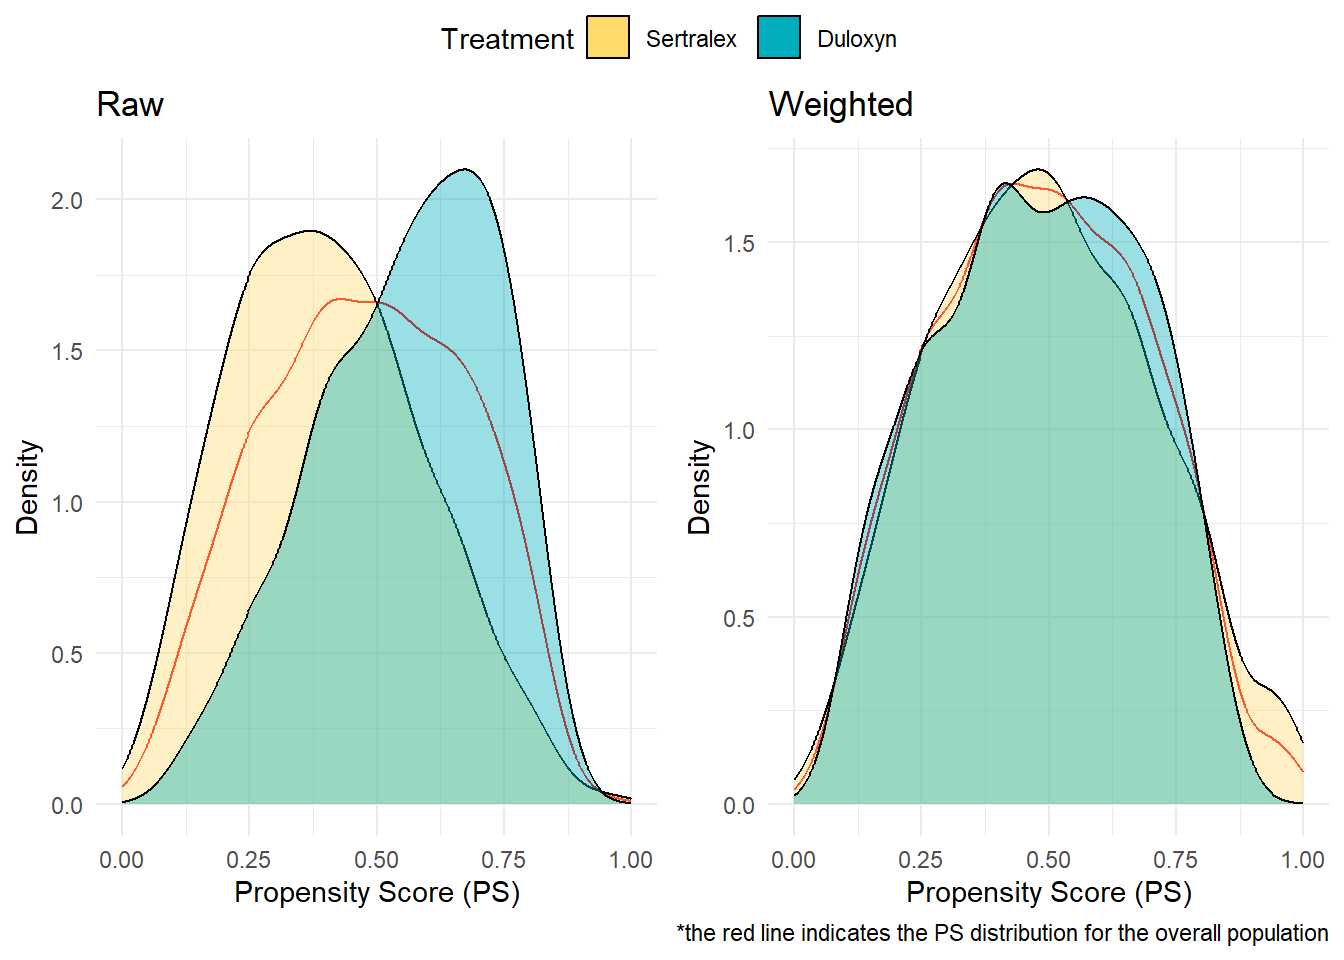
\includegraphics{_main_files/figure-latex/ps-1.pdf}

We observed that after weighting the two distributions curves align,
indicating the dataset is balanced on average.

\section{Outcome analysis}\label{outcome-analysis}

This section details the outcome analyis. First, unadjusted and weighted
Kaplan-Meier curves (\citeproc{ref-cole_adjusted_2004}{Cole and Hernán
2004}), stratified on treatment group, are compared.

\begin{Shaded}
\begin{Highlighting}[]
\CommentTok{\#Implement unadjusted model}
\NormalTok{unadjusted}\OtherTok{\textless{}{-}} \FunctionTok{survfit}\NormalTok{(}\FunctionTok{Surv}\NormalTok{(TIME\_TO\_EVENT, EVENT)}\SpecialCharTok{\textasciitilde{}}\NormalTok{TREAT, }\AttributeTok{data =}\NormalTok{ data)}
\CommentTok{\#Implement IPTW adjusted model}
\NormalTok{weighted}\OtherTok{\textless{}{-}} \FunctionTok{survfit}\NormalTok{(}\FunctionTok{Surv}\NormalTok{(TIME\_TO\_EVENT, EVENT)}\SpecialCharTok{\textasciitilde{}}\NormalTok{TREAT, }\AttributeTok{data =}\NormalTok{ data, }\AttributeTok{weights =}\NormalTok{ weights)}
\CommentTok{\#Combine both}
\NormalTok{fit}\OtherTok{\textless{}{-}}\FunctionTok{list}\NormalTok{(unadjusted,weighted)}

\CommentTok{\# Function to format survival probabilities at a given time point}
\NormalTok{format\_median\_time }\OtherTok{\textless{}{-}} \ControlFlowTok{function}\NormalTok{(surv\_object, treatment\_index) \{}
  
  \CommentTok{\# Extract the median survival time for the given treatment index}
\NormalTok{  median\_surv }\OtherTok{\textless{}{-}} \FunctionTok{sprintf}\NormalTok{(}\StringTok{"\%.2f"}\NormalTok{, }\FunctionTok{round}\NormalTok{(}\FunctionTok{summary}\NormalTok{(surv\_object)}\SpecialCharTok{$}\NormalTok{table[treatment\_index, }\StringTok{"median"}\NormalTok{], }\DecValTok{2}\NormalTok{))}
\NormalTok{  lower\_ci }\OtherTok{\textless{}{-}} \FunctionTok{sprintf}\NormalTok{(}\StringTok{"\%.2f"}\NormalTok{, }\FunctionTok{round}\NormalTok{(}\FunctionTok{summary}\NormalTok{(surv\_object)}\SpecialCharTok{$}\NormalTok{table[treatment\_index, }\StringTok{"0.95LCL"}\NormalTok{], }\DecValTok{2}\NormalTok{))}
\NormalTok{  upper\_ci }\OtherTok{\textless{}{-}} \FunctionTok{sprintf}\NormalTok{(}\StringTok{"\%.2f"}\NormalTok{, }\FunctionTok{round}\NormalTok{(}\FunctionTok{summary}\NormalTok{(surv\_object)}\SpecialCharTok{$}\NormalTok{table[treatment\_index, }\StringTok{"0.95UCL"}\NormalTok{], }\DecValTok{2}\NormalTok{))}
  
  \FunctionTok{return}\NormalTok{(}\FunctionTok{paste0}\NormalTok{(median\_surv, }\StringTok{" ["}\NormalTok{, lower\_ci, }\StringTok{"; "}\NormalTok{, upper\_ci, }\StringTok{"]"}\NormalTok{))}
  
\NormalTok{\}}

\CommentTok{\# Usage for raw and IPTW median time}
\NormalTok{unadjusted\_treatment\_0 }\OtherTok{\textless{}{-}} \FunctionTok{format\_median\_time}\NormalTok{(unadjusted, }\DecValTok{1}\NormalTok{)}
\NormalTok{unadjusted\_treatment\_1 }\OtherTok{\textless{}{-}} \FunctionTok{format\_median\_time}\NormalTok{(unadjusted, }\DecValTok{2}\NormalTok{)}
\NormalTok{weighted\_treatment\_0 }\OtherTok{\textless{}{-}} \FunctionTok{format\_median\_time}\NormalTok{(weighted, }\DecValTok{1}\NormalTok{)}
\NormalTok{weighted\_treatment\_1 }\OtherTok{\textless{}{-}} \FunctionTok{format\_median\_time}\NormalTok{(weighted, }\DecValTok{2}\NormalTok{)}

\FunctionTok{ggsurvplot\_combine}\NormalTok{(fit, }
                   \AttributeTok{data =}\NormalTok{ data,}
                   \AttributeTok{legend.title =} \StringTok{""}\NormalTok{,}
                   \AttributeTok{legend.labs =} \FunctionTok{c}\NormalTok{(}\StringTok{"Unadjusted: Sertralex"}\NormalTok{, }
                                   \StringTok{"Unadjusted: Duloxyn"}\NormalTok{,}
                                   \StringTok{"Weighted: Sertralex"}\NormalTok{, }
                                   \StringTok{"Weighted: Duloxyn"}\NormalTok{),}
                   \AttributeTok{palette =} \FunctionTok{c}\NormalTok{(}\StringTok{"\#ff331a"}\NormalTok{,}\StringTok{"\#ff80a6"}\NormalTok{,}\StringTok{"\#FFDB6D"}\NormalTok{,}\StringTok{"\#27d4ad"}\NormalTok{),}
                   \AttributeTok{conf.int =} \ConstantTok{TRUE}\NormalTok{,}
                   \AttributeTok{xlab =} \StringTok{"Time (in days)"}\NormalTok{,}
                   \AttributeTok{ggtheme =} \FunctionTok{theme\_bw}\NormalTok{())}
\end{Highlighting}
\end{Shaded}

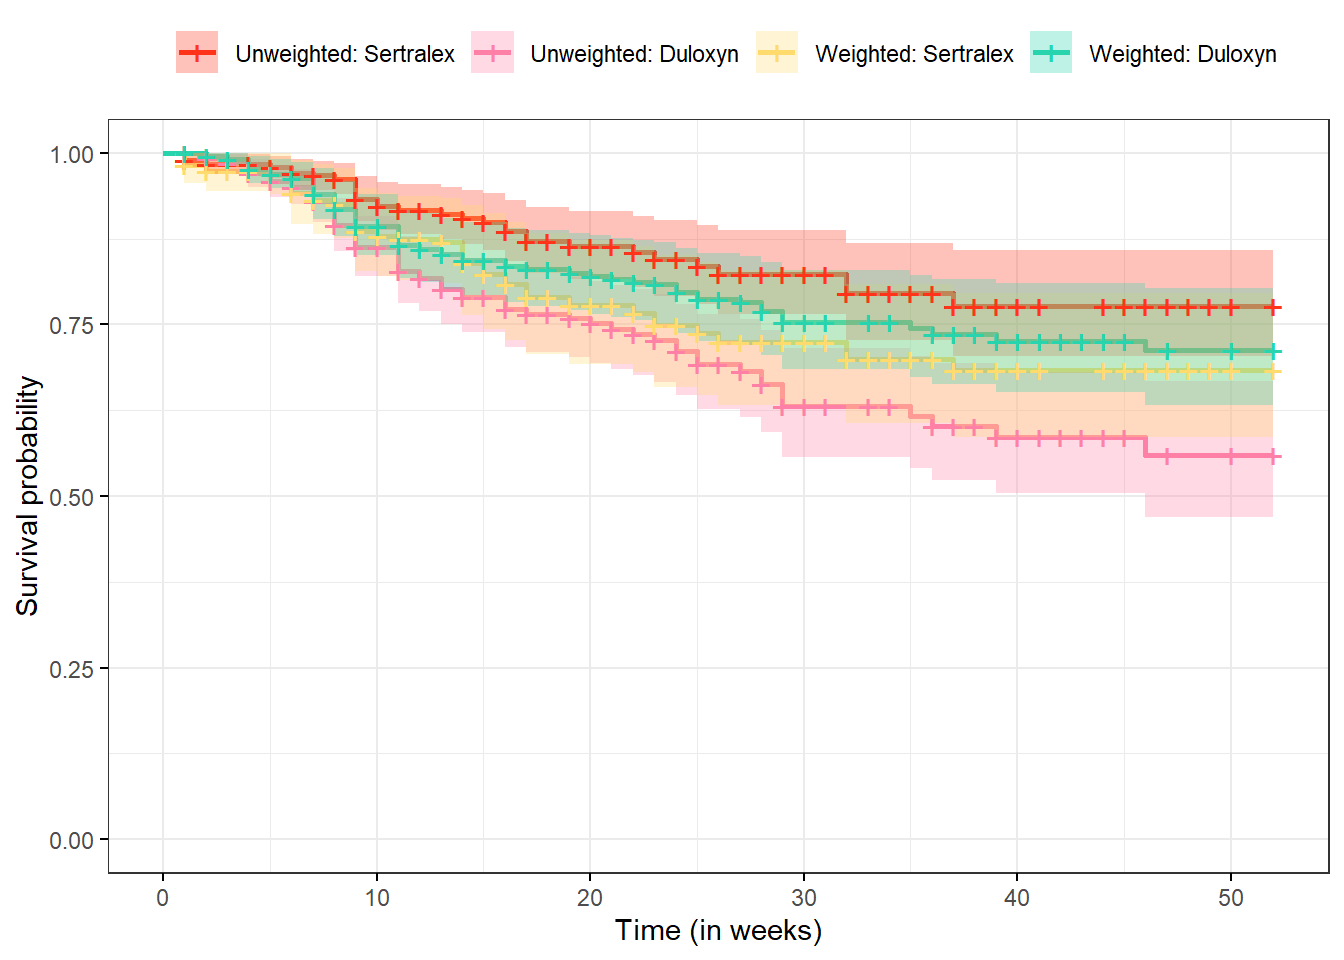
\includegraphics{_main_files/figure-latex/km-1.pdf}

As outlined, the median time to relapse differs depending on the
analysis and treatment group considered. In the unadjusted analysis, we
observed a median survival time of 67.00 {[}58.00; 84.00{]} days for
Sertralex, compared to 56.00 {[}47.00; 74.00{]} days for Duloxyn. In the
weighted analysis (where weights are used to create a pseudo
population), these differences were reduced, median survival time of
58.00 {[}46.00; 69.00{]} days for Sertralex and 64.00 {[}54.00; 91.00{]}
days for Duloxyn.

Second, unadjusted, multivariable, and weighted Cox are displayed.

\begin{Shaded}
\begin{Highlighting}[]
\CommentTok{\# Fit the Cox models}
\NormalTok{unadjusted }\OtherTok{\textless{}{-}} \FunctionTok{coxph}\NormalTok{(}\FunctionTok{Surv}\NormalTok{(TIME\_TO\_EVENT, EVENT) }\SpecialCharTok{\textasciitilde{}}\NormalTok{ TREAT, }\AttributeTok{data =}\NormalTok{ data)}
\NormalTok{multivariable }\OtherTok{\textless{}{-}} \FunctionTok{coxph}\NormalTok{(}\FunctionTok{Surv}\NormalTok{(TIME\_TO\_EVENT, EVENT) }\SpecialCharTok{\textasciitilde{}}\NormalTok{ TREAT }\SpecialCharTok{+}\NormalTok{ AGE }\SpecialCharTok{+}\NormalTok{ GENDER }\SpecialCharTok{+}\NormalTok{ SOCIO\_ECO }\SpecialCharTok{+}\NormalTok{ BECK, }\AttributeTok{data =}\NormalTok{ data)}
\NormalTok{weighted }\OtherTok{\textless{}{-}} \FunctionTok{coxph}\NormalTok{(}\FunctionTok{Surv}\NormalTok{(TIME\_TO\_EVENT, EVENT) }\SpecialCharTok{\textasciitilde{}}\NormalTok{ TREAT, }\AttributeTok{weights =}\NormalTok{ weights, }\AttributeTok{data =}\NormalTok{ data)}

\CommentTok{\# Create regression tables}
\NormalTok{unadjusted\_table }\OtherTok{\textless{}{-}}\NormalTok{ unadjusted }\SpecialCharTok{\%\textgreater{}\%} 
  \FunctionTok{tbl\_regression}\NormalTok{(}\AttributeTok{exponentiate =} \ConstantTok{TRUE}\NormalTok{,}
                 \AttributeTok{label =} \FunctionTok{list}\NormalTok{(TREAT }\SpecialCharTok{\textasciitilde{}} \StringTok{"Treatment (unadjusted)"}\NormalTok{))}

\NormalTok{multivariable\_table }\OtherTok{\textless{}{-}}\NormalTok{ multivariable }\SpecialCharTok{\%\textgreater{}\%} 
  \FunctionTok{tbl\_regression}\NormalTok{(}\AttributeTok{exponentiate =} \ConstantTok{TRUE}\NormalTok{,}
                 \AttributeTok{label =} \FunctionTok{list}\NormalTok{(TREAT }\SpecialCharTok{\textasciitilde{}} \StringTok{"Treatment (multivariable regression)"}\NormalTok{))}\SpecialCharTok{\%\textgreater{}\%}
  \FunctionTok{modify\_table\_body}\NormalTok{(}
    \SpecialCharTok{\textasciitilde{}}\NormalTok{ .x }\SpecialCharTok{\%\textgreater{}\%}\NormalTok{ dplyr}\SpecialCharTok{::}\FunctionTok{filter}\NormalTok{(variable }\SpecialCharTok{==} \StringTok{"TREAT"}\NormalTok{)}
\NormalTok{  )}

\NormalTok{weighted\_table }\OtherTok{\textless{}{-}}\NormalTok{ weighted }\SpecialCharTok{\%\textgreater{}\%} 
  \FunctionTok{tbl\_regression}\NormalTok{(}\AttributeTok{exponentiate =} \ConstantTok{TRUE}\NormalTok{,}
                 \AttributeTok{label =} \FunctionTok{list}\NormalTok{(TREAT }\SpecialCharTok{\textasciitilde{}} \StringTok{"Treatment (weighted)"}\NormalTok{))}\SpecialCharTok{\%\textgreater{}\%}
  \FunctionTok{modify\_table\_body}\NormalTok{(}
    \SpecialCharTok{\textasciitilde{}}\NormalTok{ .x }\SpecialCharTok{\%\textgreater{}\%}\NormalTok{ dplyr}\SpecialCharTok{::}\FunctionTok{filter}\NormalTok{(variable }\SpecialCharTok{==} \StringTok{"TREAT"}\NormalTok{)}
\NormalTok{  )}

\CommentTok{\# Function to extract HR and CI for a specific variable}
\NormalTok{extract\_hr\_ci }\OtherTok{\textless{}{-}} \ControlFlowTok{function}\NormalTok{(model) \{}
\NormalTok{  conf }\OtherTok{\textless{}{-}} \FunctionTok{confint}\NormalTok{(model)}
\NormalTok{  hr }\OtherTok{\textless{}{-}} \FunctionTok{sprintf}\NormalTok{(}\StringTok{"\%.2f"}\NormalTok{, }\FunctionTok{exp}\NormalTok{(model}\SpecialCharTok{$}\NormalTok{coefficients)[}\DecValTok{1}\NormalTok{])}
\NormalTok{  ci\_lower }\OtherTok{\textless{}{-}} \FunctionTok{sprintf}\NormalTok{(}\StringTok{"\%.2f"}\NormalTok{, }\FunctionTok{exp}\NormalTok{(conf)[}\DecValTok{1}\NormalTok{,}\DecValTok{1}\NormalTok{])}
\NormalTok{  ci\_upper }\OtherTok{\textless{}{-}} \FunctionTok{sprintf}\NormalTok{(}\StringTok{"\%.2f"}\NormalTok{, }\FunctionTok{exp}\NormalTok{(conf)[}\DecValTok{1}\NormalTok{,}\DecValTok{2}\NormalTok{])}
  \FunctionTok{return}\NormalTok{(}\FunctionTok{paste0}\NormalTok{(}\StringTok{"HR = "}\NormalTok{, hr, }\StringTok{" ["}\NormalTok{, ci\_lower, }\StringTok{"; "}\NormalTok{, ci\_upper, }\StringTok{"]"}\NormalTok{))}
\NormalTok{\}}

\CommentTok{\# Extract and format HR and CI for TREAT}
\NormalTok{unadjusted\_hr\_ci }\OtherTok{\textless{}{-}} \FunctionTok{extract\_hr\_ci}\NormalTok{(unadjusted)}
\NormalTok{multivariable\_hr\_ci }\OtherTok{\textless{}{-}} \FunctionTok{extract\_hr\_ci}\NormalTok{(multivariable)}
\NormalTok{weighted\_hr\_ci }\OtherTok{\textless{}{-}} \FunctionTok{extract\_hr\_ci}\NormalTok{(weighted)}

\CommentTok{\# Stack the regression tables}
\FunctionTok{tbl\_stack}\NormalTok{(}\FunctionTok{list}\NormalTok{(unadjusted\_table, multivariable\_table, weighted\_table))}
\end{Highlighting}
\end{Shaded}

\begin{table}[!t]
\fontsize{12.0pt}{14.4pt}\selectfont
\begin{tabular*}{\linewidth}{@{\extracolsep{\fill}}lccc}
\toprule
\textbf{Characteristic} & \textbf{HR}\textsuperscript{\textit{1}} & \textbf{95\% CI}\textsuperscript{\textit{1}} & \textbf{p-value} \\ 
\midrule\addlinespace[2.5pt]
Treatment (unadjusted) &  &  &  \\ 
    Sertralex & — & — &  \\ 
    Duloxyn & 1.11 & 0.92, 1.34 & 0.3 \\ 
Treatment (multivariable regression) &  &  &  \\ 
    Sertralex & — & — &  \\ 
    Duloxyn & 0.55 & 0.45, 0.68 & <0.001 \\ 
Treatment (weighted) &  &  &  \\ 
    Sertralex & — & — &  \\ 
    Duloxyn & 0.84 & 0.69, 1.03 & 0.095 \\ 
\bottomrule
\end{tabular*}
\begin{minipage}{\linewidth}
\textsuperscript{\textit{1}}HR = Hazard Ratio, CI = Confidence Interval\\
\end{minipage}
\end{table}

The results indicate that the treatment effect varies depending on the
analysis and treatment group considered. In the unadjusted analysis, the
hazard ratio (HR = 1.11 {[}0.92; 1.34{]}) suggests that Duloxyn
significantly increases the risk of relapse. In contrast, the
multivariable model reveals the opposite findings with a hazard ratio of
HR = 0.55 {[}0.45; 0.68{]}. Meanwhile, the IPTW analysis yielded
non-significant results with HR = 0.84 {[}0.69; 1.03{]}. Finally, the
slight differences between the multivariable and IPTW models demonstrate
that conditional and marginal effects are not strictly equivalent.

\chapter{Clone-Censor-Weight method}\label{clone-censor-weight}

\section{Background}\label{background-2}

Another challenge common in RWD studies, in addition to confounding, is
immortal time bias. This bias often occurs when there is a time
difference between the beginning of follow-up (time zero) and the
initiation of treatment, this is especially true when this
systematically differs across groups.

For instance, if Sertralex patients begin treatment later than Duloxyn
individuals, a form of immortal time occurs. In other words, individuals
on Duloxyn might experience an event sooner, simply due to the earlier
start of their follow-up period. This difference in initiation timing
may not be random and could, in fact, be influenced by various factors
that need to be considered into the analysis.

To address both confounding and immortal time bias, the
Clone-Censor-Weight (CCW) approach was introduced
(\citeproc{ref-hernan_specifying_2016}{Hernán et al. 2016};
\citeproc{ref-maringe_reflection_2020}{Maringe et al. 2020}). Three
common scenarios were distinguished for the use of CCW: grace periods-a
period during which treatment initiation can happen, static time-related
strategies, and dynamic strategies
(\citeproc{ref-zhao_versatility_2021}{Zhao, Lyu, and Yoshida 2021}).

The scenario 2 discussed in Chapter @ref(motivating-example) corresponds
to the grace period scenario and will be applied to illustrate the
application of CCW .

\section{CCW implementation}\label{ccw-implementation}

This code implements the CCW approach.

\subsection{Cloning}\label{cloning}

The cloning approach involves creating a duplicate of the initial
dataset, where each clone is assigned the opposite treatment.

\begin{Shaded}
\begin{Highlighting}[]
\CommentTok{\# Step 1 cloning}
\CommentTok{\# Make a copy of original data}
\NormalTok{original\_data }\OtherTok{\textless{}{-}}\NormalTok{ data}
\NormalTok{original\_data }\OtherTok{\textless{}{-}}\NormalTok{ original\_data }\SpecialCharTok{\%\textgreater{}\%}
                  \FunctionTok{mutate}\NormalTok{(}\AttributeTok{SOCIO\_ECO\_2 =} \FunctionTok{ifelse}\NormalTok{(SOCIO\_ECO }\SpecialCharTok{==} \StringTok{"Low"}\NormalTok{, }\DecValTok{1}\NormalTok{, }\DecValTok{0}\NormalTok{),}
                         \AttributeTok{SOCIO\_ECO\_3 =} \FunctionTok{ifelse}\NormalTok{(SOCIO\_ECO }\SpecialCharTok{==} \StringTok{"Moderate"}\NormalTok{, }\DecValTok{1}\NormalTok{, }\DecValTok{0}\NormalTok{),}
                         \AttributeTok{SOCIO\_ECO\_4 =} \FunctionTok{ifelse}\NormalTok{(SOCIO\_ECO }\SpecialCharTok{==} \StringTok{"High"}\NormalTok{, }\DecValTok{1}\NormalTok{, }\DecValTok{0}\NormalTok{),}
                         \AttributeTok{SOCIO\_ECO\_5 =} \FunctionTok{ifelse}\NormalTok{(SOCIO\_ECO }\SpecialCharTok{==} \StringTok{"Very high"}\NormalTok{, }\DecValTok{1}\NormalTok{, }\DecValTok{0}\NormalTok{)) }\SpecialCharTok{\%\textgreater{}\%}
  \FunctionTok{select}\NormalTok{(}\SpecialCharTok{{-}}\NormalTok{SOCIO\_ECO)}

\CommentTok{\# Create cloned data}
\NormalTok{cloned\_data }\OtherTok{\textless{}{-}}\NormalTok{ original\_data }\SpecialCharTok{\%\textgreater{}\%}
  \FunctionTok{mutate}\NormalTok{(}
    \AttributeTok{ID =}\NormalTok{ ID }\SpecialCharTok{+} \DecValTok{1000}\NormalTok{,                   }\CommentTok{\# Modify ID to differentiate cloned records}
    \AttributeTok{TREAT =} \FunctionTok{ifelse}\NormalTok{(TREAT }\SpecialCharTok{==} \StringTok{"Duloxyn"}\NormalTok{, }\StringTok{"Sertralex"}\NormalTok{, }\StringTok{"Duloxyn"}\NormalTok{)}
\NormalTok{  )         }\CommentTok{\# Remove TIME\_TO\_TREAT for clones}
\end{Highlighting}
\end{Shaded}

\subsection{Censoring}\label{censoring}

Next, the censoring pattern must be established in the dataset. In the
original dataset, no censoring is applied, whereas in the cloned
dataset, censoring is set at the time of treatment initiation. The two
datasets are then merged and reformatted to include risk intervals for
each individual, defined with start and stop times.

\begin{Shaded}
\begin{Highlighting}[]
\CommentTok{\# Step 2 censoring}
\NormalTok{original\_data }\OtherTok{\textless{}{-}}\NormalTok{ original\_data }\SpecialCharTok{\%\textgreater{}\%}
  \FunctionTok{mutate}\NormalTok{(}
    \AttributeTok{CENSOR =} \DecValTok{0}\NormalTok{,                       }\CommentTok{\# Indicator for uncensored data in the original dataset}
    \AttributeTok{TIME\_TO\_CENSOR =}\NormalTok{ TIME\_TO\_TREAT    }\CommentTok{\# Initial censoring time is set to treatment time}
\NormalTok{  ) }\SpecialCharTok{\%\textgreater{}\%}
  \FunctionTok{select}\NormalTok{(}\SpecialCharTok{{-}}\NormalTok{TIME\_TO\_TREAT)               }\CommentTok{\# Remove TIME\_TO\_TREAT for simplicity}

\NormalTok{cloned\_data }\OtherTok{\textless{}{-}}\NormalTok{ cloned\_data }\SpecialCharTok{\%\textgreater{}\%}
  \FunctionTok{mutate}\NormalTok{(}
    \AttributeTok{EVENT =} \DecValTok{0}\NormalTok{,                        }\CommentTok{\# No relapse events for cloned records}
    \AttributeTok{CENSOR =} \DecValTok{1}\NormalTok{,                       }\CommentTok{\# Cloned records are censored}
    \AttributeTok{TIME\_TO\_CENSOR =}\NormalTok{ TIME\_TO\_TREAT    }\CommentTok{\# Use TIME\_TO\_EVENT as censoring time for clones}
\NormalTok{  ) }\SpecialCharTok{\%\textgreater{}\%}
  \FunctionTok{select}\NormalTok{(}\SpecialCharTok{{-}}\NormalTok{TIME\_TO\_TREAT)               }\CommentTok{\# Remove TIME\_TO\_TREAT for clones}

\CommentTok{\# Combine original and cloned datasets}
\NormalTok{combined\_data }\OtherTok{\textless{}{-}} \FunctionTok{bind\_rows}\NormalTok{(original\_data, cloned\_data) }\SpecialCharTok{\%\textgreater{}\%}
  \FunctionTok{mutate}\NormalTok{(}
    \AttributeTok{TIME\_TO\_EVENT =}\NormalTok{ TIME\_TO\_EVENT }\SpecialCharTok{+} \FloatTok{0.001}\NormalTok{,  }\CommentTok{\# Add small increments to avoid duplicate times}
    \AttributeTok{TIME\_TO\_CENSOR =}\NormalTok{ TIME\_TO\_CENSOR }\SpecialCharTok{+} \FloatTok{0.001}\NormalTok{, }\CommentTok{\# Add small increments for censoring times}
    \AttributeTok{TSTART =} \DecValTok{0}                              \CommentTok{\# Set start time for all records}
\NormalTok{  )}

\CommentTok{\# Identify unique times for events and censoring}
\NormalTok{t\_events }\OtherTok{\textless{}{-}} \FunctionTok{sort}\NormalTok{(}\FunctionTok{unique}\NormalTok{(combined\_data}\SpecialCharTok{$}\NormalTok{TIME\_TO\_EVENT))  }\CommentTok{\# Unique event times}
\NormalTok{t\_censor }\OtherTok{\textless{}{-}} \FunctionTok{sort}\NormalTok{(}\FunctionTok{unique}\NormalTok{(combined\_data}\SpecialCharTok{$}\NormalTok{TIME\_TO\_CENSOR)) }\CommentTok{\# Unique censoring times}

\CommentTok{\# Reshape data for events using survSplit}
\NormalTok{combined\_data\_events }\OtherTok{\textless{}{-}} \FunctionTok{survSplit}\NormalTok{(}
  \FunctionTok{Surv}\NormalTok{(TSTART, TIME\_TO\_EVENT, EVENT) }\SpecialCharTok{\textasciitilde{}}\NormalTok{ ., }
  \AttributeTok{data =}\NormalTok{ combined\_data, }
  \AttributeTok{cut =}\NormalTok{ t\_events, }
  \AttributeTok{id =} \StringTok{"id"}
\NormalTok{) }\SpecialCharTok{\%\textgreater{}\%}
  \FunctionTok{rename}\NormalTok{(}\AttributeTok{TSTOP =}\NormalTok{ TIME\_TO\_EVENT) }\SpecialCharTok{\%\textgreater{}\%}
  \FunctionTok{select}\NormalTok{(ID, TREAT, TSTART, TSTOP, EVENT)    }\CommentTok{\# Keep relevant columns for events}

\CommentTok{\# Reshape data for censoring using survSplit}
\NormalTok{combined\_data\_cens }\OtherTok{\textless{}{-}} \FunctionTok{survSplit}\NormalTok{(}
  \FunctionTok{Surv}\NormalTok{(TSTART, TIME\_TO\_CENSOR, CENSOR) }\SpecialCharTok{\textasciitilde{}}\NormalTok{ ., }
  \AttributeTok{data =}\NormalTok{ combined\_data, }
  \AttributeTok{cut =}\NormalTok{ t\_censor, }
  \AttributeTok{id =} \StringTok{"id"}
\NormalTok{) }\SpecialCharTok{\%\textgreater{}\%}
  \FunctionTok{rename}\NormalTok{(}\AttributeTok{TSTOP =}\NormalTok{ TIME\_TO\_CENSOR) }\SpecialCharTok{\%\textgreater{}\%}
  \FunctionTok{select}\NormalTok{(ID, TREAT, TSTART, TSTOP, CENSOR)  }

\CommentTok{\# Extract covariates for the analysis}
\NormalTok{combined\_data\_covariate }\OtherTok{\textless{}{-}}\NormalTok{ combined\_data }\SpecialCharTok{\%\textgreater{}\%}
  \FunctionTok{select}\NormalTok{(ID, AGE, GENDER, SOCIO\_ECO\_2, SOCIO\_ECO\_3, SOCIO\_ECO\_4, SOCIO\_ECO\_5, BECK)}

\CommentTok{\# Combine event and censoring datasets}
\NormalTok{combined\_data }\OtherTok{\textless{}{-}} \FunctionTok{full\_join}\NormalTok{(}
\NormalTok{  combined\_data\_events,}
\NormalTok{  combined\_data\_cens,}
  \AttributeTok{by =} \FunctionTok{c}\NormalTok{(}\StringTok{"ID"}\NormalTok{, }\StringTok{"TREAT"}\NormalTok{, }\StringTok{"TSTART"}\NormalTok{, }\StringTok{"TSTOP"}\NormalTok{)  }\CommentTok{\# Merge by ID, treatment, start, and stop times}
\NormalTok{) }\SpecialCharTok{\%\textgreater{}\%}
  \FunctionTok{mutate}\NormalTok{(}
    \AttributeTok{EVENT =} \FunctionTok{ifelse}\NormalTok{(}\FunctionTok{is.na}\NormalTok{(EVENT), }\DecValTok{0}\NormalTok{, EVENT),   }\CommentTok{\# Replace missing EVENT values with 0}
    \AttributeTok{CENSOR =} \FunctionTok{ifelse}\NormalTok{(}\FunctionTok{is.na}\NormalTok{(CENSOR), }\DecValTok{0}\NormalTok{, CENSOR) }\CommentTok{\# Replace missing CENSOR values with 0}
\NormalTok{  ) }\SpecialCharTok{\%\textgreater{}\%}
  \FunctionTok{group\_by}\NormalTok{(ID) }\SpecialCharTok{\%\textgreater{}\%}
  \FunctionTok{mutate}\NormalTok{(}
    \AttributeTok{censor\_cumsum =} \FunctionTok{cumsum}\NormalTok{(}\FunctionTok{cumsum}\NormalTok{(CENSOR)),   }\CommentTok{\# Count cumulative censored events per ID}
    \AttributeTok{event\_cumsum =} \FunctionTok{cumsum}\NormalTok{(}\FunctionTok{cumsum}\NormalTok{(EVENT))      }\CommentTok{\# Count cumulative relapse events per ID}
\NormalTok{  ) }\SpecialCharTok{\%\textgreater{}\%}
  \FunctionTok{filter}\NormalTok{(censor\_cumsum }\SpecialCharTok{\textless{}=} \DecValTok{1} \SpecialCharTok{\&}\NormalTok{ event\_cumsum }\SpecialCharTok{\textless{}=} \DecValTok{1}\NormalTok{) }\SpecialCharTok{\%\textgreater{}\%}  \CommentTok{\# Retain only one censor or event per ID}
  \FunctionTok{select}\NormalTok{(}\SpecialCharTok{{-}}\NormalTok{censor\_cumsum, }\SpecialCharTok{{-}}\NormalTok{event\_cumsum) }\SpecialCharTok{\%\textgreater{}\%}
  \FunctionTok{inner\_join}\NormalTok{(combined\_data\_covariate, }\AttributeTok{by =} \StringTok{"ID"}\NormalTok{)}

\NormalTok{combined\_data}\SpecialCharTok{$}\NormalTok{TREAT}\OtherTok{\textless{}{-}}\FunctionTok{factor}\NormalTok{(combined\_data}\SpecialCharTok{$}\NormalTok{TREAT,}\AttributeTok{levels=}\FunctionTok{c}\NormalTok{(}\StringTok{"Sertralex"}\NormalTok{,}\StringTok{"Duloxyn"}\NormalTok{))}

\CommentTok{\# Print first individual (ID = 3) and its clone (ID = 1003)}
\NormalTok{combined\_data }\SpecialCharTok{\%\textgreater{}\%}
  \FunctionTok{filter}\NormalTok{(ID }\SpecialCharTok{\%in\%} \FunctionTok{c}\NormalTok{(}\DecValTok{3}\NormalTok{,}\DecValTok{1003}\NormalTok{)) }\SpecialCharTok{\%\textgreater{}\%}
  \FunctionTok{arrange}\NormalTok{(ID) }\SpecialCharTok{\%\textgreater{}\%}
  \FunctionTok{kbl}\NormalTok{() }\SpecialCharTok{\%\textgreater{}\%}
  \FunctionTok{kable\_styling}\NormalTok{(}\AttributeTok{font\_size =} \DecValTok{12}\NormalTok{) }\SpecialCharTok{\%\textgreater{}\%}
  \FunctionTok{scroll\_box}\NormalTok{(}\AttributeTok{width =} \StringTok{"100\%"}\NormalTok{, }\AttributeTok{height =} \StringTok{"200px"}\NormalTok{)}
\end{Highlighting}
\end{Shaded}

\begin{table}
\centering\begingroup\fontsize{12}{14}\selectfont

\begin{tabular}[t]{r|l|r|r|r|r|r|l|r|r|r|r|r}
\hline
ID & TREAT & TSTART & TSTOP & EVENT & CENSOR & AGE & GENDER & SOCIO\_ECO\_2 & SOCIO\_ECO\_3 & SOCIO\_ECO\_4 & SOCIO\_ECO\_5 & BECK\\
\hline
3 & Sertralex & 0.000 & 4.001 & 0 & 0 & 34 & Female & 0 & 0 & 0 & 1 & 23\\
\hline
3 & Sertralex & 4.001 & 5.001 & 0 & 0 & 34 & Female & 0 & 0 & 0 & 1 & 23\\
\hline
3 & Sertralex & 5.001 & 6.001 & 0 & 0 & 34 & Female & 0 & 0 & 0 & 1 & 23\\
\hline
3 & Sertralex & 6.001 & 7.001 & 0 & 0 & 34 & Female & 0 & 0 & 0 & 1 & 23\\
\hline
3 & Sertralex & 7.001 & 8.001 & 0 & 0 & 34 & Female & 0 & 0 & 0 & 1 & 23\\
\hline
3 & Sertralex & 8.001 & 9.001 & 0 & 0 & 34 & Female & 0 & 0 & 0 & 1 & 23\\
\hline
3 & Sertralex & 9.001 & 10.001 & 0 & 0 & 34 & Female & 0 & 0 & 0 & 1 & 23\\
\hline
3 & Sertralex & 10.001 & 11.001 & 0 & 0 & 34 & Female & 0 & 0 & 0 & 1 & 23\\
\hline
3 & Sertralex & 11.001 & 12.001 & 0 & 0 & 34 & Female & 0 & 0 & 0 & 1 & 23\\
\hline
3 & Sertralex & 12.001 & 13.001 & 0 & 0 & 34 & Female & 0 & 0 & 0 & 1 & 23\\
\hline
3 & Sertralex & 13.001 & 14.001 & 0 & 0 & 34 & Female & 0 & 0 & 0 & 1 & 23\\
\hline
3 & Sertralex & 14.001 & 15.001 & 0 & 0 & 34 & Female & 0 & 0 & 0 & 1 & 23\\
\hline
3 & Sertralex & 15.001 & 16.001 & 0 & 0 & 34 & Female & 0 & 0 & 0 & 1 & 23\\
\hline
3 & Sertralex & 16.001 & 17.001 & 0 & 0 & 34 & Female & 0 & 0 & 0 & 1 & 23\\
\hline
3 & Sertralex & 17.001 & 18.001 & 0 & 0 & 34 & Female & 0 & 0 & 0 & 1 & 23\\
\hline
3 & Sertralex & 18.001 & 19.001 & 0 & 0 & 34 & Female & 0 & 0 & 0 & 1 & 23\\
\hline
3 & Sertralex & 19.001 & 20.001 & 0 & 0 & 34 & Female & 0 & 0 & 0 & 1 & 23\\
\hline
3 & Sertralex & 20.001 & 21.001 & 0 & 0 & 34 & Female & 0 & 0 & 0 & 1 & 23\\
\hline
3 & Sertralex & 21.001 & 22.001 & 0 & 0 & 34 & Female & 0 & 0 & 0 & 1 & 23\\
\hline
3 & Sertralex & 22.001 & 23.001 & 0 & 0 & 34 & Female & 0 & 0 & 0 & 1 & 23\\
\hline
3 & Sertralex & 23.001 & 24.001 & 0 & 0 & 34 & Female & 0 & 0 & 0 & 1 & 23\\
\hline
3 & Sertralex & 24.001 & 25.001 & 0 & 0 & 34 & Female & 0 & 0 & 0 & 1 & 23\\
\hline
3 & Sertralex & 25.001 & 26.001 & 0 & 0 & 34 & Female & 0 & 0 & 0 & 1 & 23\\
\hline
3 & Sertralex & 26.001 & 27.001 & 0 & 0 & 34 & Female & 0 & 0 & 0 & 1 & 23\\
\hline
3 & Sertralex & 27.001 & 28.001 & 0 & 0 & 34 & Female & 0 & 0 & 0 & 1 & 23\\
\hline
3 & Sertralex & 28.001 & 29.001 & 0 & 0 & 34 & Female & 0 & 0 & 0 & 1 & 23\\
\hline
3 & Sertralex & 29.001 & 30.001 & 0 & 0 & 34 & Female & 0 & 0 & 0 & 1 & 23\\
\hline
3 & Sertralex & 30.001 & 31.001 & 0 & 0 & 34 & Female & 0 & 0 & 0 & 1 & 23\\
\hline
3 & Sertralex & 31.001 & 32.001 & 0 & 0 & 34 & Female & 0 & 0 & 0 & 1 & 23\\
\hline
3 & Sertralex & 32.001 & 33.001 & 0 & 0 & 34 & Female & 0 & 0 & 0 & 1 & 23\\
\hline
3 & Sertralex & 33.001 & 34.001 & 0 & 0 & 34 & Female & 0 & 0 & 0 & 1 & 23\\
\hline
3 & Sertralex & 34.001 & 35.001 & 0 & 0 & 34 & Female & 0 & 0 & 0 & 1 & 23\\
\hline
3 & Sertralex & 35.001 & 36.001 & 0 & 0 & 34 & Female & 0 & 0 & 0 & 1 & 23\\
\hline
3 & Sertralex & 36.001 & 37.001 & 0 & 0 & 34 & Female & 0 & 0 & 0 & 1 & 23\\
\hline
3 & Sertralex & 37.001 & 38.001 & 0 & 0 & 34 & Female & 0 & 0 & 0 & 1 & 23\\
\hline
3 & Sertralex & 38.001 & 39.001 & 0 & 0 & 34 & Female & 0 & 0 & 0 & 1 & 23\\
\hline
3 & Sertralex & 39.001 & 40.001 & 0 & 0 & 34 & Female & 0 & 0 & 0 & 1 & 23\\
\hline
3 & Sertralex & 40.001 & 41.001 & 0 & 0 & 34 & Female & 0 & 0 & 0 & 1 & 23\\
\hline
3 & Sertralex & 41.001 & 42.001 & 0 & 0 & 34 & Female & 0 & 0 & 0 & 1 & 23\\
\hline
3 & Sertralex & 42.001 & 43.001 & 0 & 0 & 34 & Female & 0 & 0 & 0 & 1 & 23\\
\hline
3 & Sertralex & 43.001 & 44.001 & 0 & 0 & 34 & Female & 0 & 0 & 0 & 1 & 23\\
\hline
3 & Sertralex & 44.001 & 45.001 & 0 & 0 & 34 & Female & 0 & 0 & 0 & 1 & 23\\
\hline
3 & Sertralex & 45.001 & 46.001 & 0 & 0 & 34 & Female & 0 & 0 & 0 & 1 & 23\\
\hline
3 & Sertralex & 46.001 & 47.001 & 0 & 0 & 34 & Female & 0 & 0 & 0 & 1 & 23\\
\hline
3 & Sertralex & 47.001 & 48.001 & 0 & 0 & 34 & Female & 0 & 0 & 0 & 1 & 23\\
\hline
3 & Sertralex & 48.001 & 49.001 & 0 & 0 & 34 & Female & 0 & 0 & 0 & 1 & 23\\
\hline
3 & Sertralex & 49.001 & 50.001 & 0 & 0 & 34 & Female & 0 & 0 & 0 & 1 & 23\\
\hline
3 & Sertralex & 50.001 & 51.001 & 0 & 0 & 34 & Female & 0 & 0 & 0 & 1 & 23\\
\hline
3 & Sertralex & 51.001 & 52.001 & 0 & 0 & 34 & Female & 0 & 0 & 0 & 1 & 23\\
\hline
3 & Sertralex & 52.001 & 53.001 & 0 & 0 & 34 & Female & 0 & 0 & 0 & 1 & 23\\
\hline
3 & Sertralex & 53.001 & 54.001 & 0 & 0 & 34 & Female & 0 & 0 & 0 & 1 & 23\\
\hline
3 & Sertralex & 54.001 & 56.001 & 0 & 0 & 34 & Female & 0 & 0 & 0 & 1 & 23\\
\hline
3 & Sertralex & 56.001 & 57.001 & 0 & 0 & 34 & Female & 0 & 0 & 0 & 1 & 23\\
\hline
3 & Sertralex & 57.001 & 58.001 & 0 & 0 & 34 & Female & 0 & 0 & 0 & 1 & 23\\
\hline
3 & Sertralex & 58.001 & 59.001 & 0 & 0 & 34 & Female & 0 & 0 & 0 & 1 & 23\\
\hline
3 & Sertralex & 59.001 & 60.001 & 0 & 0 & 34 & Female & 0 & 0 & 0 & 1 & 23\\
\hline
3 & Sertralex & 60.001 & 61.001 & 0 & 0 & 34 & Female & 0 & 0 & 0 & 1 & 23\\
\hline
3 & Sertralex & 61.001 & 62.001 & 0 & 0 & 34 & Female & 0 & 0 & 0 & 1 & 23\\
\hline
3 & Sertralex & 62.001 & 63.001 & 0 & 0 & 34 & Female & 0 & 0 & 0 & 1 & 23\\
\hline
3 & Sertralex & 63.001 & 64.001 & 0 & 0 & 34 & Female & 0 & 0 & 0 & 1 & 23\\
\hline
3 & Sertralex & 64.001 & 65.001 & 0 & 0 & 34 & Female & 0 & 0 & 0 & 1 & 23\\
\hline
3 & Sertralex & 65.001 & 66.001 & 0 & 0 & 34 & Female & 0 & 0 & 0 & 1 & 23\\
\hline
3 & Sertralex & 66.001 & 67.001 & 0 & 0 & 34 & Female & 0 & 0 & 0 & 1 & 23\\
\hline
3 & Sertralex & 67.001 & 68.001 & 0 & 0 & 34 & Female & 0 & 0 & 0 & 1 & 23\\
\hline
3 & Sertralex & 68.001 & 69.001 & 0 & 0 & 34 & Female & 0 & 0 & 0 & 1 & 23\\
\hline
3 & Sertralex & 69.001 & 70.001 & 0 & 0 & 34 & Female & 0 & 0 & 0 & 1 & 23\\
\hline
3 & Sertralex & 70.001 & 71.001 & 0 & 0 & 34 & Female & 0 & 0 & 0 & 1 & 23\\
\hline
3 & Sertralex & 71.001 & 72.001 & 0 & 0 & 34 & Female & 0 & 0 & 0 & 1 & 23\\
\hline
3 & Sertralex & 72.001 & 73.001 & 0 & 0 & 34 & Female & 0 & 0 & 0 & 1 & 23\\
\hline
3 & Sertralex & 73.001 & 74.001 & 0 & 0 & 34 & Female & 0 & 0 & 0 & 1 & 23\\
\hline
3 & Sertralex & 74.001 & 75.001 & 0 & 0 & 34 & Female & 0 & 0 & 0 & 1 & 23\\
\hline
3 & Sertralex & 75.001 & 77.001 & 0 & 0 & 34 & Female & 0 & 0 & 0 & 1 & 23\\
\hline
3 & Sertralex & 77.001 & 78.001 & 0 & 0 & 34 & Female & 0 & 0 & 0 & 1 & 23\\
\hline
3 & Sertralex & 78.001 & 79.001 & 0 & 0 & 34 & Female & 0 & 0 & 0 & 1 & 23\\
\hline
3 & Sertralex & 79.001 & 80.001 & 0 & 0 & 34 & Female & 0 & 0 & 0 & 1 & 23\\
\hline
3 & Sertralex & 80.001 & 82.001 & 0 & 0 & 34 & Female & 0 & 0 & 0 & 1 & 23\\
\hline
3 & Sertralex & 82.001 & 83.001 & 0 & 0 & 34 & Female & 0 & 0 & 0 & 1 & 23\\
\hline
3 & Sertralex & 83.001 & 84.001 & 0 & 0 & 34 & Female & 0 & 0 & 0 & 1 & 23\\
\hline
3 & Sertralex & 84.001 & 85.001 & 0 & 0 & 34 & Female & 0 & 0 & 0 & 1 & 23\\
\hline
3 & Sertralex & 85.001 & 86.001 & 0 & 0 & 34 & Female & 0 & 0 & 0 & 1 & 23\\
\hline
3 & Sertralex & 86.001 & 87.001 & 0 & 0 & 34 & Female & 0 & 0 & 0 & 1 & 23\\
\hline
3 & Sertralex & 87.001 & 88.001 & 0 & 0 & 34 & Female & 0 & 0 & 0 & 1 & 23\\
\hline
3 & Sertralex & 88.001 & 89.001 & 0 & 0 & 34 & Female & 0 & 0 & 0 & 1 & 23\\
\hline
3 & Sertralex & 89.001 & 90.001 & 0 & 0 & 34 & Female & 0 & 0 & 0 & 1 & 23\\
\hline
3 & Sertralex & 90.001 & 91.001 & 0 & 0 & 34 & Female & 0 & 0 & 0 & 1 & 23\\
\hline
3 & Sertralex & 91.001 & 92.001 & 0 & 0 & 34 & Female & 0 & 0 & 0 & 1 & 23\\
\hline
3 & Sertralex & 92.001 & 93.001 & 0 & 0 & 34 & Female & 0 & 0 & 0 & 1 & 23\\
\hline
3 & Sertralex & 93.001 & 94.001 & 0 & 0 & 34 & Female & 0 & 0 & 0 & 1 & 23\\
\hline
3 & Sertralex & 94.001 & 95.001 & 0 & 0 & 34 & Female & 0 & 0 & 0 & 1 & 23\\
\hline
3 & Sertralex & 95.001 & 97.001 & 0 & 0 & 34 & Female & 0 & 0 & 0 & 1 & 23\\
\hline
3 & Sertralex & 97.001 & 98.001 & 0 & 0 & 34 & Female & 0 & 0 & 0 & 1 & 23\\
\hline
3 & Sertralex & 98.001 & 99.001 & 0 & 0 & 34 & Female & 0 & 0 & 0 & 1 & 23\\
\hline
3 & Sertralex & 99.001 & 100.001 & 0 & 0 & 34 & Female & 0 & 0 & 0 & 1 & 23\\
\hline
3 & Sertralex & 100.001 & 101.001 & 0 & 0 & 34 & Female & 0 & 0 & 0 & 1 & 23\\
\hline
3 & Sertralex & 101.001 & 102.001 & 0 & 0 & 34 & Female & 0 & 0 & 0 & 1 & 23\\
\hline
3 & Sertralex & 102.001 & 103.001 & 0 & 0 & 34 & Female & 0 & 0 & 0 & 1 & 23\\
\hline
3 & Sertralex & 103.001 & 104.001 & 0 & 0 & 34 & Female & 0 & 0 & 0 & 1 & 23\\
\hline
3 & Sertralex & 104.001 & 105.001 & 0 & 0 & 34 & Female & 0 & 0 & 0 & 1 & 23\\
\hline
3 & Sertralex & 105.001 & 107.001 & 0 & 0 & 34 & Female & 0 & 0 & 0 & 1 & 23\\
\hline
3 & Sertralex & 107.001 & 109.001 & 0 & 0 & 34 & Female & 0 & 0 & 0 & 1 & 23\\
\hline
3 & Sertralex & 109.001 & 110.001 & 0 & 0 & 34 & Female & 0 & 0 & 0 & 1 & 23\\
\hline
3 & Sertralex & 110.001 & 111.001 & 0 & 0 & 34 & Female & 0 & 0 & 0 & 1 & 23\\
\hline
3 & Sertralex & 111.001 & 112.001 & 0 & 0 & 34 & Female & 0 & 0 & 0 & 1 & 23\\
\hline
3 & Sertralex & 112.001 & 114.001 & 0 & 0 & 34 & Female & 0 & 0 & 0 & 1 & 23\\
\hline
3 & Sertralex & 114.001 & 116.001 & 0 & 0 & 34 & Female & 0 & 0 & 0 & 1 & 23\\
\hline
3 & Sertralex & 116.001 & 118.001 & 0 & 0 & 34 & Female & 0 & 0 & 0 & 1 & 23\\
\hline
3 & Sertralex & 118.001 & 119.001 & 0 & 0 & 34 & Female & 0 & 0 & 0 & 1 & 23\\
\hline
3 & Sertralex & 119.001 & 120.001 & 0 & 0 & 34 & Female & 0 & 0 & 0 & 1 & 23\\
\hline
3 & Sertralex & 120.001 & 123.001 & 0 & 0 & 34 & Female & 0 & 0 & 0 & 1 & 23\\
\hline
3 & Sertralex & 123.001 & 127.001 & 0 & 0 & 34 & Female & 0 & 0 & 0 & 1 & 23\\
\hline
3 & Sertralex & 127.001 & 129.001 & 0 & 0 & 34 & Female & 0 & 0 & 0 & 1 & 23\\
\hline
3 & Sertralex & 129.001 & 134.001 & 0 & 0 & 34 & Female & 0 & 0 & 0 & 1 & 23\\
\hline
3 & Sertralex & 134.001 & 135.001 & 0 & 0 & 34 & Female & 0 & 0 & 0 & 1 & 23\\
\hline
3 & Sertralex & 135.001 & 137.001 & 0 & 0 & 34 & Female & 0 & 0 & 0 & 1 & 23\\
\hline
3 & Sertralex & 137.001 & 138.001 & 0 & 0 & 34 & Female & 0 & 0 & 0 & 1 & 23\\
\hline
3 & Sertralex & 138.001 & 139.001 & 0 & 0 & 34 & Female & 0 & 0 & 0 & 1 & 23\\
\hline
3 & Sertralex & 139.001 & 140.001 & 0 & 0 & 34 & Female & 0 & 0 & 0 & 1 & 23\\
\hline
3 & Sertralex & 140.001 & 141.001 & 0 & 0 & 34 & Female & 0 & 0 & 0 & 1 & 23\\
\hline
3 & Sertralex & 141.001 & 142.001 & 0 & 0 & 34 & Female & 0 & 0 & 0 & 1 & 23\\
\hline
3 & Sertralex & 142.001 & 143.001 & 0 & 0 & 34 & Female & 0 & 0 & 0 & 1 & 23\\
\hline
3 & Sertralex & 143.001 & 148.001 & 0 & 0 & 34 & Female & 0 & 0 & 0 & 1 & 23\\
\hline
3 & Sertralex & 148.001 & 150.001 & 0 & 0 & 34 & Female & 0 & 0 & 0 & 1 & 23\\
\hline
3 & Sertralex & 150.001 & 154.001 & 0 & 0 & 34 & Female & 0 & 0 & 0 & 1 & 23\\
\hline
3 & Sertralex & 154.001 & 157.001 & 0 & 0 & 34 & Female & 0 & 0 & 0 & 1 & 23\\
\hline
3 & Sertralex & 157.001 & 160.001 & 0 & 0 & 34 & Female & 0 & 0 & 0 & 1 & 23\\
\hline
3 & Sertralex & 160.001 & 161.001 & 0 & 0 & 34 & Female & 0 & 0 & 0 & 1 & 23\\
\hline
3 & Sertralex & 161.001 & 163.001 & 0 & 0 & 34 & Female & 0 & 0 & 0 & 1 & 23\\
\hline
3 & Sertralex & 163.001 & 166.001 & 0 & 0 & 34 & Female & 0 & 0 & 0 & 1 & 23\\
\hline
3 & Sertralex & 166.001 & 167.001 & 0 & 0 & 34 & Female & 0 & 0 & 0 & 1 & 23\\
\hline
3 & Sertralex & 167.001 & 171.001 & 0 & 0 & 34 & Female & 0 & 0 & 0 & 1 & 23\\
\hline
3 & Sertralex & 171.001 & 172.001 & 0 & 0 & 34 & Female & 0 & 0 & 0 & 1 & 23\\
\hline
3 & Sertralex & 172.001 & 176.001 & 0 & 0 & 34 & Female & 0 & 0 & 0 & 1 & 23\\
\hline
3 & Sertralex & 176.001 & 178.001 & 0 & 0 & 34 & Female & 0 & 0 & 0 & 1 & 23\\
\hline
3 & Sertralex & 178.001 & 179.001 & 0 & 0 & 34 & Female & 0 & 0 & 0 & 1 & 23\\
\hline
3 & Sertralex & 179.001 & 181.001 & 0 & 0 & 34 & Female & 0 & 0 & 0 & 1 & 23\\
\hline
3 & Sertralex & 181.001 & 183.001 & 0 & 0 & 34 & Female & 0 & 0 & 0 & 1 & 23\\
\hline
3 & Sertralex & 183.001 & 187.001 & 0 & 0 & 34 & Female & 0 & 0 & 0 & 1 & 23\\
\hline
3 & Sertralex & 187.001 & 188.001 & 0 & 0 & 34 & Female & 0 & 0 & 0 & 1 & 23\\
\hline
3 & Sertralex & 188.001 & 190.001 & 0 & 0 & 34 & Female & 0 & 0 & 0 & 1 & 23\\
\hline
3 & Sertralex & 190.001 & 193.001 & 0 & 0 & 34 & Female & 0 & 0 & 0 & 1 & 23\\
\hline
3 & Sertralex & 193.001 & 198.001 & 0 & 0 & 34 & Female & 0 & 0 & 0 & 1 & 23\\
\hline
3 & Sertralex & 198.001 & 200.001 & 0 & 0 & 34 & Female & 0 & 0 & 0 & 1 & 23\\
\hline
3 & Sertralex & 200.001 & 203.001 & 0 & 0 & 34 & Female & 0 & 0 & 0 & 1 & 23\\
\hline
3 & Sertralex & 203.001 & 204.001 & 0 & 0 & 34 & Female & 0 & 0 & 0 & 1 & 23\\
\hline
3 & Sertralex & 204.001 & 217.001 & 0 & 0 & 34 & Female & 0 & 0 & 0 & 1 & 23\\
\hline
3 & Sertralex & 217.001 & 218.001 & 0 & 0 & 34 & Female & 0 & 0 & 0 & 1 & 23\\
\hline
3 & Sertralex & 218.001 & 223.001 & 0 & 0 & 34 & Female & 0 & 0 & 0 & 1 & 23\\
\hline
3 & Sertralex & 223.001 & 229.001 & 0 & 0 & 34 & Female & 0 & 0 & 0 & 1 & 23\\
\hline
3 & Sertralex & 229.001 & 235.001 & 0 & 0 & 34 & Female & 0 & 0 & 0 & 1 & 23\\
\hline
3 & Sertralex & 235.001 & 238.001 & 0 & 0 & 34 & Female & 0 & 0 & 0 & 1 & 23\\
\hline
3 & Sertralex & 238.001 & 242.001 & 0 & 0 & 34 & Female & 0 & 0 & 0 & 1 & 23\\
\hline
3 & Sertralex & 242.001 & 243.001 & 0 & 0 & 34 & Female & 0 & 0 & 0 & 1 & 23\\
\hline
3 & Sertralex & 243.001 & 246.001 & 0 & 0 & 34 & Female & 0 & 0 & 0 & 1 & 23\\
\hline
3 & Sertralex & 246.001 & 249.001 & 0 & 0 & 34 & Female & 0 & 0 & 0 & 1 & 23\\
\hline
3 & Sertralex & 249.001 & 252.001 & 0 & 0 & 34 & Female & 0 & 0 & 0 & 1 & 23\\
\hline
3 & Sertralex & 252.001 & 259.001 & 0 & 0 & 34 & Female & 0 & 0 & 0 & 1 & 23\\
\hline
3 & Sertralex & 259.001 & 260.001 & 0 & 0 & 34 & Female & 0 & 0 & 0 & 1 & 23\\
\hline
3 & Sertralex & 260.001 & 261.001 & 0 & 0 & 34 & Female & 0 & 0 & 0 & 1 & 23\\
\hline
3 & Sertralex & 261.001 & 271.001 & 0 & 0 & 34 & Female & 0 & 0 & 0 & 1 & 23\\
\hline
3 & Sertralex & 271.001 & 276.001 & 0 & 0 & 34 & Female & 0 & 0 & 0 & 1 & 23\\
\hline
3 & Sertralex & 276.001 & 279.001 & 0 & 0 & 34 & Female & 0 & 0 & 0 & 1 & 23\\
\hline
3 & Sertralex & 279.001 & 285.001 & 0 & 0 & 34 & Female & 0 & 0 & 0 & 1 & 23\\
\hline
3 & Sertralex & 285.001 & 290.001 & 0 & 0 & 34 & Female & 0 & 0 & 0 & 1 & 23\\
\hline
3 & Sertralex & 290.001 & 291.001 & 0 & 0 & 34 & Female & 0 & 0 & 0 & 1 & 23\\
\hline
3 & Sertralex & 291.001 & 298.001 & 0 & 0 & 34 & Female & 0 & 0 & 0 & 1 & 23\\
\hline
3 & Sertralex & 298.001 & 308.001 & 1 & 0 & 34 & Female & 0 & 0 & 0 & 1 & 23\\
\hline
1003 & Duloxyn & 0.000 & 4.001 & 0 & 0 & 34 & Female & 0 & 0 & 0 & 1 & 23\\
\hline
1003 & Duloxyn & 4.001 & 5.001 & 0 & 0 & 34 & Female & 0 & 0 & 0 & 1 & 23\\
\hline
1003 & Duloxyn & 5.001 & 6.001 & 0 & 0 & 34 & Female & 0 & 0 & 0 & 1 & 23\\
\hline
1003 & Duloxyn & 6.001 & 7.001 & 0 & 0 & 34 & Female & 0 & 0 & 0 & 1 & 23\\
\hline
1003 & Duloxyn & 7.001 & 8.001 & 0 & 0 & 34 & Female & 0 & 0 & 0 & 1 & 23\\
\hline
1003 & Duloxyn & 8.001 & 9.001 & 0 & 0 & 34 & Female & 0 & 0 & 0 & 1 & 23\\
\hline
1003 & Duloxyn & 9.001 & 10.001 & 0 & 1 & 34 & Female & 0 & 0 & 0 & 1 & 23\\
\hline
\end{tabular}
\endgroup{}
\end{table}

\subsection{Weighting}\label{weighting}

Finally, the probability of remaining uncensored is estimated separately
using a Cox model.

\begin{Shaded}
\begin{Highlighting}[]
\CommentTok{\# Step 3 weighting}

\CommentTok{\#Filter data for the "Duloxyn" treatment group and estimate censoring probabilities}
\NormalTok{combined\_data\_duloxyn }\OtherTok{\textless{}{-}}\NormalTok{ combined\_data }\SpecialCharTok{\%\textgreater{}\%} \FunctionTok{filter}\NormalTok{(TREAT }\SpecialCharTok{==} \StringTok{"Duloxyn"}\NormalTok{)}

\CommentTok{\# Fit a Cox proportional hazards model to estimate the hazard for censoring}
\NormalTok{ms\_cens\_duloxyn }\OtherTok{\textless{}{-}} \FunctionTok{coxph}\NormalTok{(}\FunctionTok{Surv}\NormalTok{(TSTART, TSTOP, CENSOR) }\SpecialCharTok{\textasciitilde{}}\NormalTok{ AGE }\SpecialCharTok{+}\NormalTok{ GENDER }\SpecialCharTok{+}\NormalTok{ SOCIO\_ECO\_2 }\SpecialCharTok{+}\NormalTok{ SOCIO\_ECO\_3 }\SpecialCharTok{+}\NormalTok{ SOCIO\_ECO\_4 }\SpecialCharTok{+}\NormalTok{ SOCIO\_ECO\_5 }\SpecialCharTok{+}\NormalTok{ BECK, }
                         \AttributeTok{ties =} \StringTok{"efron"}\NormalTok{, }\AttributeTok{data =}\NormalTok{ combined\_data\_duloxyn)}

\CommentTok{\# Extract the baseline hazard from the Cox model}
\NormalTok{baseline\_hazard }\OtherTok{\textless{}{-}} \FunctionTok{basehaz}\NormalTok{(ms\_cens\_duloxyn, }\AttributeTok{centered =} \ConstantTok{FALSE}\NormalTok{)}

\CommentTok{\# Calculate the linear predictor (lp) for the "Duloxyn" group}
\NormalTok{combined\_data\_duloxyn}\SpecialCharTok{$}\NormalTok{lp }\OtherTok{\textless{}{-}} \FunctionTok{predict}\NormalTok{(ms\_cens\_duloxyn, }\AttributeTok{newdata =}\NormalTok{ combined\_data\_duloxyn, }\AttributeTok{type =} \StringTok{"lp"}\NormalTok{)}

\CommentTok{\# Merge the baseline hazard with the dataset based on time}
\NormalTok{combined\_data\_duloxyn }\OtherTok{\textless{}{-}} \FunctionTok{merge}\NormalTok{(combined\_data\_duloxyn, baseline\_hazard, }
                               \AttributeTok{by.x =} \StringTok{"TSTOP"}\NormalTok{, }\AttributeTok{by.y =} \StringTok{"time"}\NormalTok{, }\AttributeTok{all.x =} \ConstantTok{TRUE}\NormalTok{)}

\CommentTok{\# Calculate the uncensored probability}
\NormalTok{combined\_data\_duloxyn}\SpecialCharTok{$}\NormalTok{p\_uncens }\OtherTok{\textless{}{-}} \FunctionTok{exp}\NormalTok{(}\SpecialCharTok{{-}}\NormalTok{combined\_data\_duloxyn}\SpecialCharTok{$}\NormalTok{hazard }\SpecialCharTok{*} \FunctionTok{exp}\NormalTok{(combined\_data\_duloxyn}\SpecialCharTok{$}\NormalTok{lp))}

\CommentTok{\# Calculate the weights as the inverse of the uncensored probability}
\NormalTok{combined\_data\_duloxyn}\SpecialCharTok{$}\NormalTok{weights }\OtherTok{\textless{}{-}} \DecValTok{1} \SpecialCharTok{/}\NormalTok{ combined\_data\_duloxyn}\SpecialCharTok{$}\NormalTok{p\_uncens}

\CommentTok{\# Repeat the same process for the "Sertralex" treatment group}
\CommentTok{\# Filter data for the "Sertralex" treatment group}

\NormalTok{combined\_data\_sertralex }\OtherTok{\textless{}{-}}\NormalTok{ combined\_data }\SpecialCharTok{\%\textgreater{}\%} \FunctionTok{filter}\NormalTok{(TREAT }\SpecialCharTok{==} \StringTok{"Sertralex"}\NormalTok{)}

\CommentTok{\# Fit a Cox proportional hazards model for censoring in the "Sertralex" group}
\NormalTok{ms\_cens\_sertralex }\OtherTok{\textless{}{-}} \FunctionTok{coxph}\NormalTok{(}\FunctionTok{Surv}\NormalTok{(TSTART, TSTOP, CENSOR) }\SpecialCharTok{\textasciitilde{}}\NormalTok{ AGE }\SpecialCharTok{+}\NormalTok{ GENDER }\SpecialCharTok{+}\NormalTok{ SOCIO\_ECO\_2 }\SpecialCharTok{+}\NormalTok{ SOCIO\_ECO\_3 }\SpecialCharTok{+}\NormalTok{ SOCIO\_ECO\_4 }\SpecialCharTok{+}\NormalTok{ SOCIO\_ECO\_5 }\SpecialCharTok{+}\NormalTok{ BECK, }
                           \AttributeTok{ties =} \StringTok{"efron"}\NormalTok{, }\AttributeTok{data =}\NormalTok{ combined\_data\_sertralex)}

\CommentTok{\# Use the baseline hazard from the "Duloxyn" model (assumed shared here)}
\NormalTok{baseline\_hazard }\OtherTok{\textless{}{-}} \FunctionTok{basehaz}\NormalTok{(ms\_cens\_duloxyn, }\AttributeTok{centered =} \ConstantTok{FALSE}\NormalTok{)}

\CommentTok{\# Calculate the linear predictor (lp) for the "Sertralex" group}
\NormalTok{combined\_data\_sertralex}\SpecialCharTok{$}\NormalTok{lp }\OtherTok{\textless{}{-}} \FunctionTok{predict}\NormalTok{(ms\_cens\_sertralex, }\AttributeTok{newdata =}\NormalTok{ combined\_data\_sertralex, }\AttributeTok{type =} \StringTok{"lp"}\NormalTok{)}

\CommentTok{\# Merge the baseline hazard with the dataset based on time}
\NormalTok{combined\_data\_sertralex }\OtherTok{\textless{}{-}} \FunctionTok{merge}\NormalTok{(combined\_data\_sertralex, baseline\_hazard, }
                                 \AttributeTok{by.x =} \StringTok{"TSTOP"}\NormalTok{, }\AttributeTok{by.y =} \StringTok{"time"}\NormalTok{, }\AttributeTok{all.x =} \ConstantTok{TRUE}\NormalTok{)}

\CommentTok{\# Calculate the uncensored probability}
\NormalTok{combined\_data\_sertralex}\SpecialCharTok{$}\NormalTok{p\_uncens }\OtherTok{\textless{}{-}} \FunctionTok{exp}\NormalTok{(}\SpecialCharTok{{-}}\NormalTok{combined\_data\_sertralex}\SpecialCharTok{$}\NormalTok{hazard }\SpecialCharTok{*} \FunctionTok{exp}\NormalTok{(combined\_data\_sertralex}\SpecialCharTok{$}\NormalTok{lp))}

\CommentTok{\# Calculate the weights as the inverse of the uncensored probability}
\NormalTok{combined\_data\_sertralex}\SpecialCharTok{$}\NormalTok{weights }\OtherTok{\textless{}{-}} \DecValTok{1} \SpecialCharTok{/}\NormalTok{ combined\_data\_sertralex}\SpecialCharTok{$}\NormalTok{p\_uncens}

\CommentTok{\# Combine the datasets for "Duloxyn" and "Sertralex" treatments with the calculated weights}
\NormalTok{combined\_data }\OtherTok{\textless{}{-}} \FunctionTok{rbind}\NormalTok{(combined\_data\_duloxyn, combined\_data\_sertralex)}

\CommentTok{\# Display the first individual (ID = 3) and its clone (ID = 1003) with improved visualization}
\NormalTok{combined\_data }\SpecialCharTok{\%\textgreater{}\%}
  \FunctionTok{filter}\NormalTok{(ID }\SpecialCharTok{\%in\%} \FunctionTok{c}\NormalTok{(}\DecValTok{3}\NormalTok{, }\DecValTok{1003}\NormalTok{)) }\SpecialCharTok{\%\textgreater{}\%}
  \FunctionTok{arrange}\NormalTok{(ID) }\SpecialCharTok{\%\textgreater{}\%}
  \FunctionTok{kbl}\NormalTok{() }\SpecialCharTok{\%\textgreater{}\%}
  \FunctionTok{kable\_styling}\NormalTok{(}\AttributeTok{font\_size =} \DecValTok{12}\NormalTok{) }\SpecialCharTok{\%\textgreater{}\%}
  \FunctionTok{scroll\_box}\NormalTok{(}\AttributeTok{width =} \StringTok{"100\%"}\NormalTok{, }\AttributeTok{height =} \StringTok{"200px"}\NormalTok{)}
\end{Highlighting}
\end{Shaded}

\begin{table}
\centering\begingroup\fontsize{12}{14}\selectfont

\begin{tabular}[t]{r|r|l|r|r|r|r|l|r|r|r|r|r|r|r|r|r}
\hline
TSTOP & ID & TREAT & TSTART & EVENT & CENSOR & AGE & GENDER & SOCIO\_ECO\_2 & SOCIO\_ECO\_3 & SOCIO\_ECO\_4 & SOCIO\_ECO\_5 & BECK & lp & hazard & p\_uncens & weights\\
\hline
4.001 & 3 & Sertralex & 0.000 & 0 & 0 & 34 & Female & 0 & 0 & 0 & 1 & 23 & -0.3269311 & 0.0353463 & 0.9748327 & 1.025817\\
\hline
5.001 & 3 & Sertralex & 4.001 & 0 & 0 & 34 & Female & 0 & 0 & 0 & 1 & 23 & -0.3269311 & 0.0897951 & 0.9372978 & 1.066897\\
\hline
6.001 & 3 & Sertralex & 5.001 & 0 & 0 & 34 & Female & 0 & 0 & 0 & 1 & 23 & -0.3269311 & 0.1618184 & 0.8898586 & 1.123774\\
\hline
7.001 & 3 & Sertralex & 6.001 & 0 & 0 & 34 & Female & 0 & 0 & 0 & 1 & 23 & -0.3269311 & 0.2280559 & 0.8483527 & 1.178755\\
\hline
8.001 & 3 & Sertralex & 7.001 & 0 & 0 & 34 & Female & 0 & 0 & 0 & 1 & 23 & -0.3269311 & 0.3461736 & 0.7790833 & 1.283560\\
\hline
9.001 & 3 & Sertralex & 8.001 & 0 & 0 & 34 & Female & 0 & 0 & 0 & 1 & 23 & -0.3269311 & 0.4478113 & 0.7240233 & 1.381171\\
\hline
10.001 & 3 & Sertralex & 9.001 & 0 & 0 & 34 & Female & 0 & 0 & 0 & 1 & 23 & -0.3269311 & 0.5468552 & 0.6741144 & 1.483428\\
\hline
11.001 & 3 & Sertralex & 10.001 & 0 & 0 & 34 & Female & 0 & 0 & 0 & 1 & 23 & -0.3269311 & 0.6352811 & 0.6324701 & 1.581103\\
\hline
12.001 & 3 & Sertralex & 11.001 & 0 & 0 & 34 & Female & 0 & 0 & 0 & 1 & 23 & -0.3269311 & 0.6745200 & 0.6148242 & 1.626481\\
\hline
13.001 & 3 & Sertralex & 12.001 & 0 & 0 & 34 & Female & 0 & 0 & 0 & 1 & 23 & -0.3269311 & 0.6894336 & 0.6082474 & 1.644068\\
\hline
14.001 & 3 & Sertralex & 13.001 & 0 & 0 & 34 & Female & 0 & 0 & 0 & 1 & 23 & -0.3269311 & 0.7130222 & 0.5979883 & 1.672274\\
\hline
15.001 & 3 & Sertralex & 14.001 & 0 & 0 & 34 & Female & 0 & 0 & 0 & 1 & 23 & -0.3269311 & 0.7209293 & 0.5945882 & 1.681836\\
\hline
16.001 & 3 & Sertralex & 15.001 & 0 & 0 & 34 & Female & 0 & 0 & 0 & 1 & 23 & -0.3269311 & 0.7248048 & 0.5929288 & 1.686543\\
\hline
17.001 & 3 & Sertralex & 16.001 & 0 & 0 & 34 & Female & 0 & 0 & 0 & 1 & 23 & -0.3269311 & 0.7248048 & 0.5929288 & 1.686543\\
\hline
18.001 & 3 & Sertralex & 17.001 & 0 & 0 & 34 & Female & 0 & 0 & 0 & 1 & 23 & -0.3269311 & 0.7248048 & 0.5929288 & 1.686543\\
\hline
19.001 & 3 & Sertralex & 18.001 & 0 & 0 & 34 & Female & 0 & 0 & 0 & 1 & 23 & -0.3269311 & 0.7248048 & 0.5929288 & 1.686543\\
\hline
20.001 & 3 & Sertralex & 19.001 & 0 & 0 & 34 & Female & 0 & 0 & 0 & 1 & 23 & -0.3269311 & 0.7248048 & 0.5929288 & 1.686543\\
\hline
21.001 & 3 & Sertralex & 20.001 & 0 & 0 & 34 & Female & 0 & 0 & 0 & 1 & 23 & -0.3269311 & 0.7248048 & 0.5929288 & 1.686543\\
\hline
22.001 & 3 & Sertralex & 21.001 & 0 & 0 & 34 & Female & 0 & 0 & 0 & 1 & 23 & -0.3269311 & 0.7248048 & 0.5929288 & 1.686543\\
\hline
23.001 & 3 & Sertralex & 22.001 & 0 & 0 & 34 & Female & 0 & 0 & 0 & 1 & 23 & -0.3269311 & 0.7248048 & 0.5929288 & 1.686543\\
\hline
24.001 & 3 & Sertralex & 23.001 & 0 & 0 & 34 & Female & 0 & 0 & 0 & 1 & 23 & -0.3269311 & 0.7248048 & 0.5929288 & 1.686543\\
\hline
25.001 & 3 & Sertralex & 24.001 & 0 & 0 & 34 & Female & 0 & 0 & 0 & 1 & 23 & -0.3269311 & 0.7248048 & 0.5929288 & 1.686543\\
\hline
26.001 & 3 & Sertralex & 25.001 & 0 & 0 & 34 & Female & 0 & 0 & 0 & 1 & 23 & -0.3269311 & 0.7248048 & 0.5929288 & 1.686543\\
\hline
27.001 & 3 & Sertralex & 26.001 & 0 & 0 & 34 & Female & 0 & 0 & 0 & 1 & 23 & -0.3269311 & 0.7248048 & 0.5929288 & 1.686543\\
\hline
28.001 & 3 & Sertralex & 27.001 & 0 & 0 & 34 & Female & 0 & 0 & 0 & 1 & 23 & -0.3269311 & 0.7248048 & 0.5929288 & 1.686543\\
\hline
29.001 & 3 & Sertralex & 28.001 & 0 & 0 & 34 & Female & 0 & 0 & 0 & 1 & 23 & -0.3269311 & 0.7248048 & 0.5929288 & 1.686543\\
\hline
30.001 & 3 & Sertralex & 29.001 & 0 & 0 & 34 & Female & 0 & 0 & 0 & 1 & 23 & -0.3269311 & 0.7248048 & 0.5929288 & 1.686543\\
\hline
31.001 & 3 & Sertralex & 30.001 & 0 & 0 & 34 & Female & 0 & 0 & 0 & 1 & 23 & -0.3269311 & 0.7248048 & 0.5929288 & 1.686543\\
\hline
32.001 & 3 & Sertralex & 31.001 & 0 & 0 & 34 & Female & 0 & 0 & 0 & 1 & 23 & -0.3269311 & 0.7248048 & 0.5929288 & 1.686543\\
\hline
33.001 & 3 & Sertralex & 32.001 & 0 & 0 & 34 & Female & 0 & 0 & 0 & 1 & 23 & -0.3269311 & 0.7248048 & 0.5929288 & 1.686543\\
\hline
34.001 & 3 & Sertralex & 33.001 & 0 & 0 & 34 & Female & 0 & 0 & 0 & 1 & 23 & -0.3269311 & 0.7248048 & 0.5929288 & 1.686543\\
\hline
35.001 & 3 & Sertralex & 34.001 & 0 & 0 & 34 & Female & 0 & 0 & 0 & 1 & 23 & -0.3269311 & 0.7248048 & 0.5929288 & 1.686543\\
\hline
36.001 & 3 & Sertralex & 35.001 & 0 & 0 & 34 & Female & 0 & 0 & 0 & 1 & 23 & -0.3269311 & 0.7248048 & 0.5929288 & 1.686543\\
\hline
37.001 & 3 & Sertralex & 36.001 & 0 & 0 & 34 & Female & 0 & 0 & 0 & 1 & 23 & -0.3269311 & 0.7248048 & 0.5929288 & 1.686543\\
\hline
38.001 & 3 & Sertralex & 37.001 & 0 & 0 & 34 & Female & 0 & 0 & 0 & 1 & 23 & -0.3269311 & 0.7248048 & 0.5929288 & 1.686543\\
\hline
39.001 & 3 & Sertralex & 38.001 & 0 & 0 & 34 & Female & 0 & 0 & 0 & 1 & 23 & -0.3269311 & 0.7248048 & 0.5929288 & 1.686543\\
\hline
40.001 & 3 & Sertralex & 39.001 & 0 & 0 & 34 & Female & 0 & 0 & 0 & 1 & 23 & -0.3269311 & 0.7248048 & 0.5929288 & 1.686543\\
\hline
41.001 & 3 & Sertralex & 40.001 & 0 & 0 & 34 & Female & 0 & 0 & 0 & 1 & 23 & -0.3269311 & 0.7248048 & 0.5929288 & 1.686543\\
\hline
42.001 & 3 & Sertralex & 41.001 & 0 & 0 & 34 & Female & 0 & 0 & 0 & 1 & 23 & -0.3269311 & 0.7248048 & 0.5929288 & 1.686543\\
\hline
43.001 & 3 & Sertralex & 42.001 & 0 & 0 & 34 & Female & 0 & 0 & 0 & 1 & 23 & -0.3269311 & 0.7248048 & 0.5929288 & 1.686543\\
\hline
44.001 & 3 & Sertralex & 43.001 & 0 & 0 & 34 & Female & 0 & 0 & 0 & 1 & 23 & -0.3269311 & 0.7248048 & 0.5929288 & 1.686543\\
\hline
45.001 & 3 & Sertralex & 44.001 & 0 & 0 & 34 & Female & 0 & 0 & 0 & 1 & 23 & -0.3269311 & 0.7248048 & 0.5929288 & 1.686543\\
\hline
46.001 & 3 & Sertralex & 45.001 & 0 & 0 & 34 & Female & 0 & 0 & 0 & 1 & 23 & -0.3269311 & 0.7248048 & 0.5929288 & 1.686543\\
\hline
47.001 & 3 & Sertralex & 46.001 & 0 & 0 & 34 & Female & 0 & 0 & 0 & 1 & 23 & -0.3269311 & 0.7248048 & 0.5929288 & 1.686543\\
\hline
48.001 & 3 & Sertralex & 47.001 & 0 & 0 & 34 & Female & 0 & 0 & 0 & 1 & 23 & -0.3269311 & 0.7248048 & 0.5929288 & 1.686543\\
\hline
49.001 & 3 & Sertralex & 48.001 & 0 & 0 & 34 & Female & 0 & 0 & 0 & 1 & 23 & -0.3269311 & 0.7248048 & 0.5929288 & 1.686543\\
\hline
50.001 & 3 & Sertralex & 49.001 & 0 & 0 & 34 & Female & 0 & 0 & 0 & 1 & 23 & -0.3269311 & 0.7248048 & 0.5929288 & 1.686543\\
\hline
51.001 & 3 & Sertralex & 50.001 & 0 & 0 & 34 & Female & 0 & 0 & 0 & 1 & 23 & -0.3269311 & 0.7248048 & 0.5929288 & 1.686543\\
\hline
52.001 & 3 & Sertralex & 51.001 & 0 & 0 & 34 & Female & 0 & 0 & 0 & 1 & 23 & -0.3269311 & 0.7248048 & 0.5929288 & 1.686543\\
\hline
53.001 & 3 & Sertralex & 52.001 & 0 & 0 & 34 & Female & 0 & 0 & 0 & 1 & 23 & -0.3269311 & 0.7248048 & 0.5929288 & 1.686543\\
\hline
54.001 & 3 & Sertralex & 53.001 & 0 & 0 & 34 & Female & 0 & 0 & 0 & 1 & 23 & -0.3269311 & 0.7248048 & 0.5929288 & 1.686543\\
\hline
56.001 & 3 & Sertralex & 54.001 & 0 & 0 & 34 & Female & 0 & 0 & 0 & 1 & 23 & -0.3269311 & 0.7248048 & 0.5929288 & 1.686543\\
\hline
57.001 & 3 & Sertralex & 56.001 & 0 & 0 & 34 & Female & 0 & 0 & 0 & 1 & 23 & -0.3269311 & 0.7248048 & 0.5929288 & 1.686543\\
\hline
58.001 & 3 & Sertralex & 57.001 & 0 & 0 & 34 & Female & 0 & 0 & 0 & 1 & 23 & -0.3269311 & 0.7248048 & 0.5929288 & 1.686543\\
\hline
59.001 & 3 & Sertralex & 58.001 & 0 & 0 & 34 & Female & 0 & 0 & 0 & 1 & 23 & -0.3269311 & 0.7248048 & 0.5929288 & 1.686543\\
\hline
60.001 & 3 & Sertralex & 59.001 & 0 & 0 & 34 & Female & 0 & 0 & 0 & 1 & 23 & -0.3269311 & 0.7248048 & 0.5929288 & 1.686543\\
\hline
61.001 & 3 & Sertralex & 60.001 & 0 & 0 & 34 & Female & 0 & 0 & 0 & 1 & 23 & -0.3269311 & 0.7248048 & 0.5929288 & 1.686543\\
\hline
62.001 & 3 & Sertralex & 61.001 & 0 & 0 & 34 & Female & 0 & 0 & 0 & 1 & 23 & -0.3269311 & 0.7248048 & 0.5929288 & 1.686543\\
\hline
63.001 & 3 & Sertralex & 62.001 & 0 & 0 & 34 & Female & 0 & 0 & 0 & 1 & 23 & -0.3269311 & 0.7248048 & 0.5929288 & 1.686543\\
\hline
64.001 & 3 & Sertralex & 63.001 & 0 & 0 & 34 & Female & 0 & 0 & 0 & 1 & 23 & -0.3269311 & 0.7248048 & 0.5929288 & 1.686543\\
\hline
65.001 & 3 & Sertralex & 64.001 & 0 & 0 & 34 & Female & 0 & 0 & 0 & 1 & 23 & -0.3269311 & 0.7248048 & 0.5929288 & 1.686543\\
\hline
66.001 & 3 & Sertralex & 65.001 & 0 & 0 & 34 & Female & 0 & 0 & 0 & 1 & 23 & -0.3269311 & 0.7248048 & 0.5929288 & 1.686543\\
\hline
67.001 & 3 & Sertralex & 66.001 & 0 & 0 & 34 & Female & 0 & 0 & 0 & 1 & 23 & -0.3269311 & 0.7248048 & 0.5929288 & 1.686543\\
\hline
68.001 & 3 & Sertralex & 67.001 & 0 & 0 & 34 & Female & 0 & 0 & 0 & 1 & 23 & -0.3269311 & 0.7248048 & 0.5929288 & 1.686543\\
\hline
69.001 & 3 & Sertralex & 68.001 & 0 & 0 & 34 & Female & 0 & 0 & 0 & 1 & 23 & -0.3269311 & 0.7248048 & 0.5929288 & 1.686543\\
\hline
70.001 & 3 & Sertralex & 69.001 & 0 & 0 & 34 & Female & 0 & 0 & 0 & 1 & 23 & -0.3269311 & 0.7248048 & 0.5929288 & 1.686543\\
\hline
71.001 & 3 & Sertralex & 70.001 & 0 & 0 & 34 & Female & 0 & 0 & 0 & 1 & 23 & -0.3269311 & 0.7248048 & 0.5929288 & 1.686543\\
\hline
72.001 & 3 & Sertralex & 71.001 & 0 & 0 & 34 & Female & 0 & 0 & 0 & 1 & 23 & -0.3269311 & 0.7248048 & 0.5929288 & 1.686543\\
\hline
73.001 & 3 & Sertralex & 72.001 & 0 & 0 & 34 & Female & 0 & 0 & 0 & 1 & 23 & -0.3269311 & 0.7248048 & 0.5929288 & 1.686543\\
\hline
74.001 & 3 & Sertralex & 73.001 & 0 & 0 & 34 & Female & 0 & 0 & 0 & 1 & 23 & -0.3269311 & 0.7248048 & 0.5929288 & 1.686543\\
\hline
75.001 & 3 & Sertralex & 74.001 & 0 & 0 & 34 & Female & 0 & 0 & 0 & 1 & 23 & -0.3269311 & 0.7248048 & 0.5929288 & 1.686543\\
\hline
77.001 & 3 & Sertralex & 75.001 & 0 & 0 & 34 & Female & 0 & 0 & 0 & 1 & 23 & -0.3269311 & 0.7248048 & 0.5929288 & 1.686543\\
\hline
78.001 & 3 & Sertralex & 77.001 & 0 & 0 & 34 & Female & 0 & 0 & 0 & 1 & 23 & -0.3269311 & 0.7248048 & 0.5929288 & 1.686543\\
\hline
79.001 & 3 & Sertralex & 78.001 & 0 & 0 & 34 & Female & 0 & 0 & 0 & 1 & 23 & -0.3269311 & 0.7248048 & 0.5929288 & 1.686543\\
\hline
80.001 & 3 & Sertralex & 79.001 & 0 & 0 & 34 & Female & 0 & 0 & 0 & 1 & 23 & -0.3269311 & 0.7248048 & 0.5929288 & 1.686543\\
\hline
82.001 & 3 & Sertralex & 80.001 & 0 & 0 & 34 & Female & 0 & 0 & 0 & 1 & 23 & -0.3269311 & 0.7248048 & 0.5929288 & 1.686543\\
\hline
83.001 & 3 & Sertralex & 82.001 & 0 & 0 & 34 & Female & 0 & 0 & 0 & 1 & 23 & -0.3269311 & 0.7248048 & 0.5929288 & 1.686543\\
\hline
84.001 & 3 & Sertralex & 83.001 & 0 & 0 & 34 & Female & 0 & 0 & 0 & 1 & 23 & -0.3269311 & 0.7248048 & 0.5929288 & 1.686543\\
\hline
85.001 & 3 & Sertralex & 84.001 & 0 & 0 & 34 & Female & 0 & 0 & 0 & 1 & 23 & -0.3269311 & 0.7248048 & 0.5929288 & 1.686543\\
\hline
86.001 & 3 & Sertralex & 85.001 & 0 & 0 & 34 & Female & 0 & 0 & 0 & 1 & 23 & -0.3269311 & 0.7248048 & 0.5929288 & 1.686543\\
\hline
87.001 & 3 & Sertralex & 86.001 & 0 & 0 & 34 & Female & 0 & 0 & 0 & 1 & 23 & -0.3269311 & 0.7248048 & 0.5929288 & 1.686543\\
\hline
88.001 & 3 & Sertralex & 87.001 & 0 & 0 & 34 & Female & 0 & 0 & 0 & 1 & 23 & -0.3269311 & 0.7248048 & 0.5929288 & 1.686543\\
\hline
89.001 & 3 & Sertralex & 88.001 & 0 & 0 & 34 & Female & 0 & 0 & 0 & 1 & 23 & -0.3269311 & 0.7248048 & 0.5929288 & 1.686543\\
\hline
90.001 & 3 & Sertralex & 89.001 & 0 & 0 & 34 & Female & 0 & 0 & 0 & 1 & 23 & -0.3269311 & 0.7248048 & 0.5929288 & 1.686543\\
\hline
91.001 & 3 & Sertralex & 90.001 & 0 & 0 & 34 & Female & 0 & 0 & 0 & 1 & 23 & -0.3269311 & 0.7248048 & 0.5929288 & 1.686543\\
\hline
92.001 & 3 & Sertralex & 91.001 & 0 & 0 & 34 & Female & 0 & 0 & 0 & 1 & 23 & -0.3269311 & 0.7248048 & 0.5929288 & 1.686543\\
\hline
93.001 & 3 & Sertralex & 92.001 & 0 & 0 & 34 & Female & 0 & 0 & 0 & 1 & 23 & -0.3269311 & 0.7248048 & 0.5929288 & 1.686543\\
\hline
94.001 & 3 & Sertralex & 93.001 & 0 & 0 & 34 & Female & 0 & 0 & 0 & 1 & 23 & -0.3269311 & 0.7248048 & 0.5929288 & 1.686543\\
\hline
95.001 & 3 & Sertralex & 94.001 & 0 & 0 & 34 & Female & 0 & 0 & 0 & 1 & 23 & -0.3269311 & 0.7248048 & 0.5929288 & 1.686543\\
\hline
97.001 & 3 & Sertralex & 95.001 & 0 & 0 & 34 & Female & 0 & 0 & 0 & 1 & 23 & -0.3269311 & 0.7248048 & 0.5929288 & 1.686543\\
\hline
98.001 & 3 & Sertralex & 97.001 & 0 & 0 & 34 & Female & 0 & 0 & 0 & 1 & 23 & -0.3269311 & 0.7248048 & 0.5929288 & 1.686543\\
\hline
99.001 & 3 & Sertralex & 98.001 & 0 & 0 & 34 & Female & 0 & 0 & 0 & 1 & 23 & -0.3269311 & 0.7248048 & 0.5929288 & 1.686543\\
\hline
100.001 & 3 & Sertralex & 99.001 & 0 & 0 & 34 & Female & 0 & 0 & 0 & 1 & 23 & -0.3269311 & 0.7248048 & 0.5929288 & 1.686543\\
\hline
101.001 & 3 & Sertralex & 100.001 & 0 & 0 & 34 & Female & 0 & 0 & 0 & 1 & 23 & -0.3269311 & 0.7248048 & 0.5929288 & 1.686543\\
\hline
102.001 & 3 & Sertralex & 101.001 & 0 & 0 & 34 & Female & 0 & 0 & 0 & 1 & 23 & -0.3269311 & 0.7248048 & 0.5929288 & 1.686543\\
\hline
103.001 & 3 & Sertralex & 102.001 & 0 & 0 & 34 & Female & 0 & 0 & 0 & 1 & 23 & -0.3269311 & 0.7248048 & 0.5929288 & 1.686543\\
\hline
104.001 & 3 & Sertralex & 103.001 & 0 & 0 & 34 & Female & 0 & 0 & 0 & 1 & 23 & -0.3269311 & 0.7248048 & 0.5929288 & 1.686543\\
\hline
105.001 & 3 & Sertralex & 104.001 & 0 & 0 & 34 & Female & 0 & 0 & 0 & 1 & 23 & -0.3269311 & 0.7248048 & 0.5929288 & 1.686543\\
\hline
107.001 & 3 & Sertralex & 105.001 & 0 & 0 & 34 & Female & 0 & 0 & 0 & 1 & 23 & -0.3269311 & 0.7248048 & 0.5929288 & 1.686543\\
\hline
109.001 & 3 & Sertralex & 107.001 & 0 & 0 & 34 & Female & 0 & 0 & 0 & 1 & 23 & -0.3269311 & 0.7248048 & 0.5929288 & 1.686543\\
\hline
110.001 & 3 & Sertralex & 109.001 & 0 & 0 & 34 & Female & 0 & 0 & 0 & 1 & 23 & -0.3269311 & 0.7248048 & 0.5929288 & 1.686543\\
\hline
111.001 & 3 & Sertralex & 110.001 & 0 & 0 & 34 & Female & 0 & 0 & 0 & 1 & 23 & -0.3269311 & 0.7248048 & 0.5929288 & 1.686543\\
\hline
112.001 & 3 & Sertralex & 111.001 & 0 & 0 & 34 & Female & 0 & 0 & 0 & 1 & 23 & -0.3269311 & 0.7248048 & 0.5929288 & 1.686543\\
\hline
114.001 & 3 & Sertralex & 112.001 & 0 & 0 & 34 & Female & 0 & 0 & 0 & 1 & 23 & -0.3269311 & 0.7248048 & 0.5929288 & 1.686543\\
\hline
116.001 & 3 & Sertralex & 114.001 & 0 & 0 & 34 & Female & 0 & 0 & 0 & 1 & 23 & -0.3269311 & 0.7248048 & 0.5929288 & 1.686543\\
\hline
118.001 & 3 & Sertralex & 116.001 & 0 & 0 & 34 & Female & 0 & 0 & 0 & 1 & 23 & -0.3269311 & 0.7248048 & 0.5929288 & 1.686543\\
\hline
119.001 & 3 & Sertralex & 118.001 & 0 & 0 & 34 & Female & 0 & 0 & 0 & 1 & 23 & -0.3269311 & 0.7248048 & 0.5929288 & 1.686543\\
\hline
120.001 & 3 & Sertralex & 119.001 & 0 & 0 & 34 & Female & 0 & 0 & 0 & 1 & 23 & -0.3269311 & 0.7248048 & 0.5929288 & 1.686543\\
\hline
123.001 & 3 & Sertralex & 120.001 & 0 & 0 & 34 & Female & 0 & 0 & 0 & 1 & 23 & -0.3269311 & 0.7248048 & 0.5929288 & 1.686543\\
\hline
127.001 & 3 & Sertralex & 123.001 & 0 & 0 & 34 & Female & 0 & 0 & 0 & 1 & 23 & -0.3269311 & 0.7248048 & 0.5929288 & 1.686543\\
\hline
129.001 & 3 & Sertralex & 127.001 & 0 & 0 & 34 & Female & 0 & 0 & 0 & 1 & 23 & -0.3269311 & 0.7248048 & 0.5929288 & 1.686543\\
\hline
134.001 & 3 & Sertralex & 129.001 & 0 & 0 & 34 & Female & 0 & 0 & 0 & 1 & 23 & -0.3269311 & 0.7248048 & 0.5929288 & 1.686543\\
\hline
135.001 & 3 & Sertralex & 134.001 & 0 & 0 & 34 & Female & 0 & 0 & 0 & 1 & 23 & -0.3269311 & 0.7248048 & 0.5929288 & 1.686543\\
\hline
137.001 & 3 & Sertralex & 135.001 & 0 & 0 & 34 & Female & 0 & 0 & 0 & 1 & 23 & -0.3269311 & 0.7248048 & 0.5929288 & 1.686543\\
\hline
138.001 & 3 & Sertralex & 137.001 & 0 & 0 & 34 & Female & 0 & 0 & 0 & 1 & 23 & -0.3269311 & 0.7248048 & 0.5929288 & 1.686543\\
\hline
139.001 & 3 & Sertralex & 138.001 & 0 & 0 & 34 & Female & 0 & 0 & 0 & 1 & 23 & -0.3269311 & 0.7248048 & 0.5929288 & 1.686543\\
\hline
140.001 & 3 & Sertralex & 139.001 & 0 & 0 & 34 & Female & 0 & 0 & 0 & 1 & 23 & -0.3269311 & 0.7248048 & 0.5929288 & 1.686543\\
\hline
141.001 & 3 & Sertralex & 140.001 & 0 & 0 & 34 & Female & 0 & 0 & 0 & 1 & 23 & -0.3269311 & 0.7248048 & 0.5929288 & 1.686543\\
\hline
142.001 & 3 & Sertralex & 141.001 & 0 & 0 & 34 & Female & 0 & 0 & 0 & 1 & 23 & -0.3269311 & 0.7248048 & 0.5929288 & 1.686543\\
\hline
143.001 & 3 & Sertralex & 142.001 & 0 & 0 & 34 & Female & 0 & 0 & 0 & 1 & 23 & -0.3269311 & 0.7248048 & 0.5929288 & 1.686543\\
\hline
148.001 & 3 & Sertralex & 143.001 & 0 & 0 & 34 & Female & 0 & 0 & 0 & 1 & 23 & -0.3269311 & 0.7248048 & 0.5929288 & 1.686543\\
\hline
150.001 & 3 & Sertralex & 148.001 & 0 & 0 & 34 & Female & 0 & 0 & 0 & 1 & 23 & -0.3269311 & 0.7248048 & 0.5929288 & 1.686543\\
\hline
154.001 & 3 & Sertralex & 150.001 & 0 & 0 & 34 & Female & 0 & 0 & 0 & 1 & 23 & -0.3269311 & 0.7248048 & 0.5929288 & 1.686543\\
\hline
157.001 & 3 & Sertralex & 154.001 & 0 & 0 & 34 & Female & 0 & 0 & 0 & 1 & 23 & -0.3269311 & 0.7248048 & 0.5929288 & 1.686543\\
\hline
160.001 & 3 & Sertralex & 157.001 & 0 & 0 & 34 & Female & 0 & 0 & 0 & 1 & 23 & -0.3269311 & 0.7248048 & 0.5929288 & 1.686543\\
\hline
161.001 & 3 & Sertralex & 160.001 & 0 & 0 & 34 & Female & 0 & 0 & 0 & 1 & 23 & -0.3269311 & 0.7248048 & 0.5929288 & 1.686543\\
\hline
163.001 & 3 & Sertralex & 161.001 & 0 & 0 & 34 & Female & 0 & 0 & 0 & 1 & 23 & -0.3269311 & 0.7248048 & 0.5929288 & 1.686543\\
\hline
166.001 & 3 & Sertralex & 163.001 & 0 & 0 & 34 & Female & 0 & 0 & 0 & 1 & 23 & -0.3269311 & 0.7248048 & 0.5929288 & 1.686543\\
\hline
167.001 & 3 & Sertralex & 166.001 & 0 & 0 & 34 & Female & 0 & 0 & 0 & 1 & 23 & -0.3269311 & 0.7248048 & 0.5929288 & 1.686543\\
\hline
171.001 & 3 & Sertralex & 167.001 & 0 & 0 & 34 & Female & 0 & 0 & 0 & 1 & 23 & -0.3269311 & 0.7248048 & 0.5929288 & 1.686543\\
\hline
172.001 & 3 & Sertralex & 171.001 & 0 & 0 & 34 & Female & 0 & 0 & 0 & 1 & 23 & -0.3269311 & 0.7248048 & 0.5929288 & 1.686543\\
\hline
176.001 & 3 & Sertralex & 172.001 & 0 & 0 & 34 & Female & 0 & 0 & 0 & 1 & 23 & -0.3269311 & 0.7248048 & 0.5929288 & 1.686543\\
\hline
178.001 & 3 & Sertralex & 176.001 & 0 & 0 & 34 & Female & 0 & 0 & 0 & 1 & 23 & -0.3269311 & 0.7248048 & 0.5929288 & 1.686543\\
\hline
179.001 & 3 & Sertralex & 178.001 & 0 & 0 & 34 & Female & 0 & 0 & 0 & 1 & 23 & -0.3269311 & 0.7248048 & 0.5929288 & 1.686543\\
\hline
181.001 & 3 & Sertralex & 179.001 & 0 & 0 & 34 & Female & 0 & 0 & 0 & 1 & 23 & -0.3269311 & 0.7248048 & 0.5929288 & 1.686543\\
\hline
183.001 & 3 & Sertralex & 181.001 & 0 & 0 & 34 & Female & 0 & 0 & 0 & 1 & 23 & -0.3269311 & 0.7248048 & 0.5929288 & 1.686543\\
\hline
187.001 & 3 & Sertralex & 183.001 & 0 & 0 & 34 & Female & 0 & 0 & 0 & 1 & 23 & -0.3269311 & 0.7248048 & 0.5929288 & 1.686543\\
\hline
188.001 & 3 & Sertralex & 187.001 & 0 & 0 & 34 & Female & 0 & 0 & 0 & 1 & 23 & -0.3269311 & 0.7248048 & 0.5929288 & 1.686543\\
\hline
190.001 & 3 & Sertralex & 188.001 & 0 & 0 & 34 & Female & 0 & 0 & 0 & 1 & 23 & -0.3269311 & 0.7248048 & 0.5929288 & 1.686543\\
\hline
193.001 & 3 & Sertralex & 190.001 & 0 & 0 & 34 & Female & 0 & 0 & 0 & 1 & 23 & -0.3269311 & 0.7248048 & 0.5929288 & 1.686543\\
\hline
198.001 & 3 & Sertralex & 193.001 & 0 & 0 & 34 & Female & 0 & 0 & 0 & 1 & 23 & -0.3269311 & 0.7248048 & 0.5929288 & 1.686543\\
\hline
200.001 & 3 & Sertralex & 198.001 & 0 & 0 & 34 & Female & 0 & 0 & 0 & 1 & 23 & -0.3269311 & 0.7248048 & 0.5929288 & 1.686543\\
\hline
203.001 & 3 & Sertralex & 200.001 & 0 & 0 & 34 & Female & 0 & 0 & 0 & 1 & 23 & -0.3269311 & 0.7248048 & 0.5929288 & 1.686543\\
\hline
204.001 & 3 & Sertralex & 203.001 & 0 & 0 & 34 & Female & 0 & 0 & 0 & 1 & 23 & -0.3269311 & 0.7248048 & 0.5929288 & 1.686543\\
\hline
217.001 & 3 & Sertralex & 204.001 & 0 & 0 & 34 & Female & 0 & 0 & 0 & 1 & 23 & -0.3269311 & 0.7248048 & 0.5929288 & 1.686543\\
\hline
218.001 & 3 & Sertralex & 217.001 & 0 & 0 & 34 & Female & 0 & 0 & 0 & 1 & 23 & -0.3269311 & 0.7248048 & 0.5929288 & 1.686543\\
\hline
223.001 & 3 & Sertralex & 218.001 & 0 & 0 & 34 & Female & 0 & 0 & 0 & 1 & 23 & -0.3269311 & 0.7248048 & 0.5929288 & 1.686543\\
\hline
229.001 & 3 & Sertralex & 223.001 & 0 & 0 & 34 & Female & 0 & 0 & 0 & 1 & 23 & -0.3269311 & 0.7248048 & 0.5929288 & 1.686543\\
\hline
235.001 & 3 & Sertralex & 229.001 & 0 & 0 & 34 & Female & 0 & 0 & 0 & 1 & 23 & -0.3269311 & 0.7248048 & 0.5929288 & 1.686543\\
\hline
238.001 & 3 & Sertralex & 235.001 & 0 & 0 & 34 & Female & 0 & 0 & 0 & 1 & 23 & -0.3269311 & 0.7248048 & 0.5929288 & 1.686543\\
\hline
242.001 & 3 & Sertralex & 238.001 & 0 & 0 & 34 & Female & 0 & 0 & 0 & 1 & 23 & -0.3269311 & 0.7248048 & 0.5929288 & 1.686543\\
\hline
243.001 & 3 & Sertralex & 242.001 & 0 & 0 & 34 & Female & 0 & 0 & 0 & 1 & 23 & -0.3269311 & 0.7248048 & 0.5929288 & 1.686543\\
\hline
246.001 & 3 & Sertralex & 243.001 & 0 & 0 & 34 & Female & 0 & 0 & 0 & 1 & 23 & -0.3269311 & 0.7248048 & 0.5929288 & 1.686543\\
\hline
249.001 & 3 & Sertralex & 246.001 & 0 & 0 & 34 & Female & 0 & 0 & 0 & 1 & 23 & -0.3269311 & 0.7248048 & 0.5929288 & 1.686543\\
\hline
252.001 & 3 & Sertralex & 249.001 & 0 & 0 & 34 & Female & 0 & 0 & 0 & 1 & 23 & -0.3269311 & 0.7248048 & 0.5929288 & 1.686543\\
\hline
259.001 & 3 & Sertralex & 252.001 & 0 & 0 & 34 & Female & 0 & 0 & 0 & 1 & 23 & -0.3269311 & 0.7248048 & 0.5929288 & 1.686543\\
\hline
260.001 & 3 & Sertralex & 259.001 & 0 & 0 & 34 & Female & 0 & 0 & 0 & 1 & 23 & -0.3269311 & 0.7248048 & 0.5929288 & 1.686543\\
\hline
261.001 & 3 & Sertralex & 260.001 & 0 & 0 & 34 & Female & 0 & 0 & 0 & 1 & 23 & -0.3269311 & 0.7248048 & 0.5929288 & 1.686543\\
\hline
271.001 & 3 & Sertralex & 261.001 & 0 & 0 & 34 & Female & 0 & 0 & 0 & 1 & 23 & -0.3269311 & 0.7248048 & 0.5929288 & 1.686543\\
\hline
276.001 & 3 & Sertralex & 271.001 & 0 & 0 & 34 & Female & 0 & 0 & 0 & 1 & 23 & -0.3269311 & 0.7248048 & 0.5929288 & 1.686543\\
\hline
279.001 & 3 & Sertralex & 276.001 & 0 & 0 & 34 & Female & 0 & 0 & 0 & 1 & 23 & -0.3269311 & 0.7248048 & 0.5929288 & 1.686543\\
\hline
285.001 & 3 & Sertralex & 279.001 & 0 & 0 & 34 & Female & 0 & 0 & 0 & 1 & 23 & -0.3269311 & 0.7248048 & 0.5929288 & 1.686543\\
\hline
290.001 & 3 & Sertralex & 285.001 & 0 & 0 & 34 & Female & 0 & 0 & 0 & 1 & 23 & -0.3269311 & 0.7248048 & 0.5929288 & 1.686543\\
\hline
291.001 & 3 & Sertralex & 290.001 & 0 & 0 & 34 & Female & 0 & 0 & 0 & 1 & 23 & -0.3269311 & 0.7248048 & 0.5929288 & 1.686543\\
\hline
298.001 & 3 & Sertralex & 291.001 & 0 & 0 & 34 & Female & 0 & 0 & 0 & 1 & 23 & -0.3269311 & 0.7248048 & 0.5929288 & 1.686543\\
\hline
308.001 & 3 & Sertralex & 298.001 & 1 & 0 & 34 & Female & 0 & 0 & 0 & 1 & 23 & -0.3269311 & 0.7248048 & 0.5929288 & 1.686543\\
\hline
4.001 & 1003 & Duloxyn & 0.000 & 0 & 0 & 34 & Female & 0 & 0 & 0 & 1 & 23 & 0.2421007 & 0.0360903 & 0.9550646 & 1.047050\\
\hline
5.001 & 1003 & Duloxyn & 4.001 & 0 & 0 & 34 & Female & 0 & 0 & 0 & 1 & 23 & 0.2421007 & 0.0921679 & 0.8892163 & 1.124586\\
\hline
6.001 & 1003 & Duloxyn & 5.001 & 0 & 0 & 34 & Female & 0 & 0 & 0 & 1 & 23 & 0.2421007 & 0.1644918 & 0.8109493 & 1.233123\\
\hline
7.001 & 1003 & Duloxyn & 6.001 & 0 & 0 & 34 & Female & 0 & 0 & 0 & 1 & 23 & 0.2421007 & 0.2329759 & 0.7431977 & 1.345537\\
\hline
8.001 & 1003 & Duloxyn & 7.001 & 0 & 0 & 34 & Female & 0 & 0 & 0 & 1 & 23 & 0.2421007 & 0.3543962 & 0.6366895 & 1.570624\\
\hline
9.001 & 1003 & Duloxyn & 8.001 & 0 & 0 & 34 & Female & 0 & 0 & 0 & 1 & 23 & 0.2421007 & 0.4598797 & 0.5566319 & 1.796519\\
\hline
10.001 & 1003 & Duloxyn & 9.001 & 0 & 1 & 34 & Female & 0 & 0 & 0 & 1 & 23 & 0.2421007 & 0.5589815 & 0.4906133 & 2.038265\\
\hline
\end{tabular}
\endgroup{}
\end{table}

\section{Outcome analysis}\label{outcome-analysis-1}

First, the KM model is implemented.

\begin{Shaded}
\begin{Highlighting}[]
\CommentTok{\#Implement CCW  model}
\NormalTok{ccw}\OtherTok{\textless{}{-}} \FunctionTok{survfit}\NormalTok{(}\FunctionTok{Surv}\NormalTok{(TSTART, TSTOP, EVENT) }\SpecialCharTok{\textasciitilde{}}\NormalTok{ TREAT, }\AttributeTok{data =}\NormalTok{ combined\_data, }\AttributeTok{weights =}\NormalTok{ weights)}

\CommentTok{\# Calculate median survival time}
\NormalTok{ccw\_treatment\_0 }\OtherTok{\textless{}{-}} \FunctionTok{format\_median\_time}\NormalTok{(ccw, }\DecValTok{1}\NormalTok{)}
\NormalTok{ccw\_treatment\_1 }\OtherTok{\textless{}{-}} \FunctionTok{format\_median\_time}\NormalTok{(ccw, }\DecValTok{2}\NormalTok{)}

\FunctionTok{ggsurvplot}\NormalTok{(ccw, }
           \AttributeTok{data =}\NormalTok{ combined\_data,}
           \AttributeTok{legend.title =} \StringTok{""}\NormalTok{,}
           \AttributeTok{legend.labs =} \FunctionTok{c}\NormalTok{(}\StringTok{"CCW: Sertralex"}\NormalTok{,}
                           \StringTok{"CCW: Duloxyn"}\NormalTok{),}
           \AttributeTok{palette =} \FunctionTok{c}\NormalTok{(}\StringTok{"\#5A8DEE"}\NormalTok{,}\StringTok{"\#F28C2C"}\NormalTok{),}
           \AttributeTok{conf.int =} \ConstantTok{TRUE}\NormalTok{,}
           \AttributeTok{xlab =} \StringTok{"Time (in days)"}\NormalTok{,}
           \AttributeTok{ggtheme =} \FunctionTok{theme\_bw}\NormalTok{())}
\end{Highlighting}
\end{Shaded}

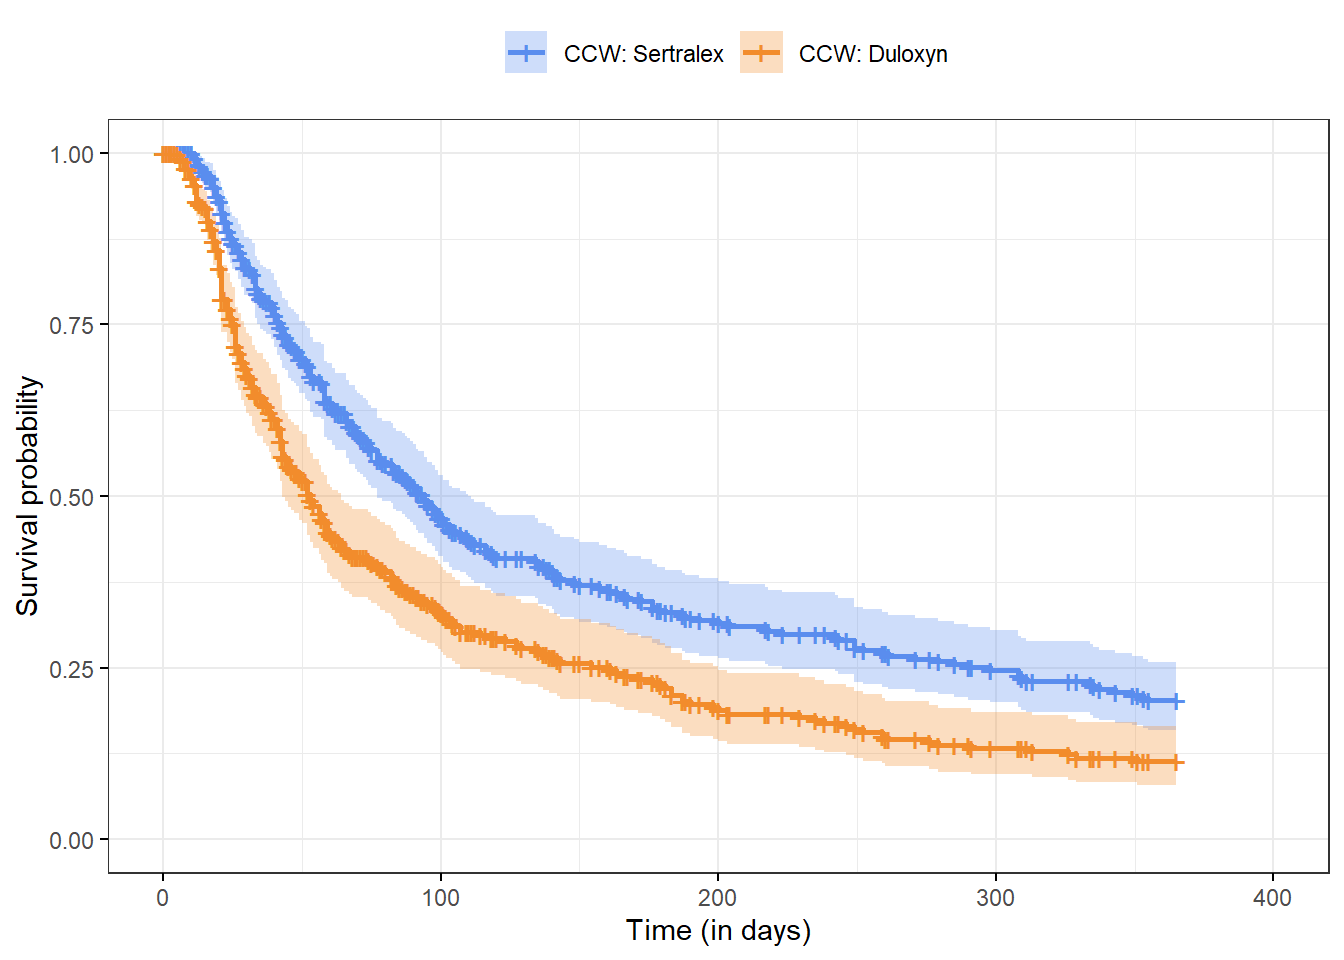
\includegraphics{_main_files/figure-latex/ccw_km-1.pdf}

In the CCW approach, the estimated median survival time in the Sertralex
population is estimated at 51.00 {[}40.00; 62.00{]} and 68.00 {[}56.00;
93.00{]} in the Duloxyn population.

Next, the Cox model is implemented where weights are considered into the
analysis.

\begin{Shaded}
\begin{Highlighting}[]
\CommentTok{\# Fit the Cox models}
\NormalTok{combined\_data}\SpecialCharTok{$}\NormalTok{TREAT }\OtherTok{\textless{}{-}} \FunctionTok{relevel}\NormalTok{(combined\_data}\SpecialCharTok{$}\NormalTok{TREAT,}\AttributeTok{ref=}\StringTok{"Sertralex"}\NormalTok{)}
\NormalTok{CCW\_cox }\OtherTok{\textless{}{-}} \FunctionTok{coxph}\NormalTok{(}\FunctionTok{Surv}\NormalTok{(TSTART, TSTOP, EVENT) }\SpecialCharTok{\textasciitilde{}}\NormalTok{ TREAT, }\AttributeTok{data =}\NormalTok{ combined\_data, }\AttributeTok{weights =}\NormalTok{ weights)}

\CommentTok{\# Create regression tables}
\NormalTok{CCW\_cox }\SpecialCharTok{\%\textgreater{}\%} 
  \FunctionTok{tbl\_regression}\NormalTok{(}\AttributeTok{exponentiate =} \ConstantTok{TRUE}\NormalTok{,}
                 \AttributeTok{label =} \FunctionTok{list}\NormalTok{(TREAT }\SpecialCharTok{\textasciitilde{}} \StringTok{"Treatment (CCW approach)"}\NormalTok{))}
\end{Highlighting}
\end{Shaded}

\begin{table}[!t]
\fontsize{12.0pt}{14.4pt}\selectfont
\begin{tabular*}{\linewidth}{@{\extracolsep{\fill}}lccc}
\toprule
\textbf{Characteristic} & \textbf{HR}\textsuperscript{\textit{1}} & \textbf{95\% CI}\textsuperscript{\textit{1}} & \textbf{p-value} \\ 
\midrule\addlinespace[2.5pt]
Treatment (CCW approach) &  &  &  \\ 
    Sertralex & — & — &  \\ 
    Duloxyn & 0.71 & 0.58, 0.88 & 0.002 \\ 
\bottomrule
\end{tabular*}
\begin{minipage}{\linewidth}
\textsuperscript{\textit{1}}HR = Hazard Ratio, CI = Confidence Interval\\
\end{minipage}
\end{table}

\begin{Shaded}
\begin{Highlighting}[]
\NormalTok{ccw\_hr\_ci }\OtherTok{\textless{}{-}} \FunctionTok{extract\_hr\_ci}\NormalTok{(CCW\_cox)}
\end{Highlighting}
\end{Shaded}

After adjusting for immortal time bias, the estimated treatment effect
is represented by HR = 0.71 {[}0.58; 0.88{]}, indicating that the
association becomes significant. This finding aligns with the simulation
process, which modeled a average difference in treatment initiation of 5
days (15 days for Duloxyn and 10 days for Sertralex), thereby offering a
survival advantage for Duloxyn users.

\chapter*{Conclusion}\label{conclusion}
\addcontentsline{toc}{chapter}{Conclusion}

As highlighted, careful consideration is essential when using RWD to
generate RWE that complements the findings of RCTs. However, following
guidance on its application and the use of appropriate statistical
methods are crucial to ensuring the reliability and robustness of its
conclusions.

\chapter*{References}\label{references}
\addcontentsline{toc}{chapter}{References}

\phantomsection\label{refs}
\begin{CSLReferences}{1}{0}
\bibitem[\citeproctext]{ref-austin_balance_2009}
Austin, Peter C. 2009. {``Balance Diagnostics for Comparing the
Distribution of Baseline Covariates Between Treatment Groups in
Propensity-Score Matched Samples.''} \emph{Statistics in Medicine} 28
(25): 3083. \url{https://doi.org/10.1002/sim.3697}.

\bibitem[\citeproctext]{ref-austin_introduction_2011}
---------. 2011. {``An Introduction to Propensity Score Methods for
Reducing the Effects of Confounding in Observational Studies.''}
\emph{Multivariate Behavioral Research} 46 (3): 399.
\url{https://doi.org/10.1080/00273171.2011.568786}.

\bibitem[\citeproctext]{ref-austin_conditioning_2007}
Austin, Peter C., Paul Grootendorst, Sharon-Lise T. Normand, and
Geoffrey M. Anderson. 2007. {``Conditioning on the Propensity Score Can
Result in Biased Estimation of Common Measures of Treatment Effect: A
Monte Carlo Study.''} \emph{Statistics in Medicine} 26 (4): 754--68.
\url{https://doi.org/10.1002/sim.2618}.

\bibitem[\citeproctext]{ref-austin_moving_2015}
Austin, Peter C., and Elizabeth A. Stuart. 2015. {``Moving Towards Best
Practice When Using Inverse Probability of Treatment Weighting ({IPTW})
Using the Propensity Score to Estimate Causal Treatment Effects in
Observational Studies.''} \emph{Statistics in Medicine} 34 (28):
3661--79. \url{https://doi.org/10.1002/sim.6607}.

\bibitem[\citeproctext]{ref-baumfeld_andre_trial_2020}
Baumfeld Andre, Elodie, Robert Reynolds, Patrick Caubel, Laurent
Azoulay, and Nancy A. Dreyer. 2020. {``Trial Designs Using Real‐world
Data: The Changing Landscape of the Regulatory Approval Process.''}
\emph{Pharmacoepidemiology and Drug Safety} 29 (10): 1201--12.
\url{https://doi.org/10.1002/pds.4932}.

\bibitem[\citeproctext]{ref-cole_adjusted_2004}
Cole, Stephen R., and Miguel A. Hernán. 2004. {``Adjusted Survival
Curves with Inverse Probability Weights.''} \emph{Computer Methods and
Programs in Biomedicine} 75 (1): 45--49.
\url{https://doi.org/10.1016/j.cmpb.2003.10.004}.

\bibitem[\citeproctext]{ref-ema_2024}
EMA. 2023. {``Real-World Evidence Framework to Support EU Regulatory
Decision-Making.''} European Medicines Agency (EMA). 2023.
\url{https://www.ema.europa.eu/en/documents/report/real-world-evidence-framework-support-eu-regulatory-decision-making-report-experience-gained-regulator-led-studies-september-2021-february-2023_en.pdf}.

\bibitem[\citeproctext]{ref-encepp_2010}
ENCePP. 2010. {``The European Network of Centres for
Pharmacoepidemiology and Pharmacovigilance ({ENCePP}) Guide on
Methodological Standards in Pharmacoepidemiology - Revision 11.''}
\emph{Guidance Document}.

\bibitem[\citeproctext]{ref-fda_real-world_2024}
FDA. 2018. {``Real-World Evidence. {FDA}.''} 2018.
\url{https://www.fda.gov/science-research/science-and-research-special-topics/real-world-evidence}.

\bibitem[\citeproctext]{ref-fda_considerations}
---------. 2023. {``Considerations for the Use of Real-World Data and
Real-World Evidence to Support Regulatory Decision-Making for Drug and
Biological Products.''} \emph{Guidance Document}.
\url{https://www.fda.gov/media/154714/download}.

\bibitem[\citeproctext]{ref-franklin_emulating_2021}
Franklin, Jessica M., Elisabetta Patorno, Rishi J. Desai, Robert J.
Glynn, David Martin, Kenneth Quinto, Ajinkya Pawar, et al. 2021.
{``Emulating Randomized Clinical Trials with Nonrandomized Real-World
Evidence Studies: First Results from the {RCT} {DUPLICATE}
Initiative.''} \emph{Circulation} 143 (10): 1002--13.
\url{https://doi.org/10.1161/CIRCULATIONAHA.120.051718}.

\bibitem[\citeproctext]{ref-funk_doubly_2011}
Funk, Michele Jonsson, Daniel Westreich, Chris Wiesen, Til Stürmer, M.
Alan Brookhart, and Marie Davidian. 2011. {``Doubly Robust Estimation of
Causal Effects.''} \emph{American Journal of Epidemiology} 173 (7): 761.
\url{https://doi.org/10.1093/aje/kwq439}.

\bibitem[\citeproctext]{ref-garrido_methods_2014}
Garrido, Melissa M., Amy S. Kelley, Julia Paris, Katherine Roza, Diane
E. Meier, R. Sean Morrison, and Melissa D. Aldridge. 2014. {``Methods
for Constructing and Assessing Propensity Scores.''} \emph{Health
Services Research} 49 (5): 1701.
\url{https://doi.org/10.1111/1475-6773.12182}.

\bibitem[\citeproctext]{ref-greifer_choosing_2023}
Greifer, Noah, and Elizabeth A. Stuart. 2023. {``Choosing the Causal
Estimand for Propensity Score Analysis of Observational Studies.''}
{arXiv}. \url{https://doi.org/10.48550/arXiv.2106.10577}.

\bibitem[\citeproctext]{ref-heiss_demystifying_nodate}
Heiss, Andrew. n.d. {``Demystifying Causal Inference Estimands: {ATE},
{ATT}, and {ATU}. Andrew Heiss.''} Accessed November 4, 2024.
\url{https://www.andrewheiss.com/blog/2024/03/21/demystifying-ate-att-atu/}.

\bibitem[\citeproctext]{ref-hernan_causal_nodate}
Hernan, Miguel A, and James M Robins. 2024. {``Causal Inference: What
If,''} January.

\bibitem[\citeproctext]{ref-hernan_using_2016}
Hernán, Miguel A., and James M. Robins. 2016. {``Using Big Data to
Emulate a Target Trial When a Randomized Trial Is Not Available.''}
\emph{American Journal of Epidemiology} 183 (8): 758--64.
\url{https://doi.org/10.1093/aje/kwv254}.

\bibitem[\citeproctext]{ref-hernan_specifying_2016}
Hernán, Miguel A., Brian C. Sauer, Sonia Hernández-Díaz, Robert Platt,
and Ian Shrier. 2016. {``Specifying a Target Trial Prevents Immortal
Time Bias and Other Self-Inflicted Injuries in Observational
Analyses.''} \emph{Journal of Clinical Epidemiology} 79 (November):
70--75. \url{https://doi.org/10.1016/j.jclinepi.2016.04.014}.

\bibitem[\citeproctext]{ref-noauthor_ich_1998}
{``ICH E9 R1 Addendum.''} 2020. July 30, 2020.
\url{https://www.ema.europa.eu/en/ich-e9-statistical-principles-clinical-trials-scientific-guideline}.

\bibitem[\citeproctext]{ref-khosla_real_2018}
Khosla, Sajan, Robert White, Jesús Medina, Mario Ouwens, Cathy Emmas,
Tim Koder, Gary Male, and Sandra Leonard. 2018. {``Real World Evidence
({RWE}) -- a Disruptive Innovation or the Quiet Evolution of Medical
Evidence Generation?''} \emph{F1000Research} 7 (August): 111.
\url{https://doi.org/10.12688/f1000research.13585.2}.

\bibitem[\citeproctext]{ref-lawrance_what_2020}
Lawrance, Rachael, Evgeny Degtyarev, Philip Griffiths, Peter Trask,
Helen Lau, Denise D'Alessio, Ingolf Griebsch, Gudrun Wallenstein, Kim
Cocks, and Kaspar Rufibach. 2020. {``What Is an Estimand \& How Does It
Relate to Quantifying the Effect of Treatment on Patient-Reported
Quality of Life Outcomes in Clinical Trials?''} \emph{Journal of
Patient-Reported Outcomes} 4 (1): 68.
\url{https://doi.org/10.1186/s41687-020-00218-5}.

\bibitem[\citeproctext]{ref-mackinnon_unification_2021}
MacKinnon, David P., and Sophia J. Lamp. 2021. {``A Unification of
Mediator, Confounder, and Collider Effects.''} \emph{Prevention Science
: The Official Journal of the Society for Prevention Research} 22 (8):
1185. \url{https://doi.org/10.1007/s11121-021-01268-x}.

\bibitem[\citeproctext]{ref-maringe_reflection_2020}
Maringe, Camille, Sara Benitez Majano, Aimilia Exarchakou, Matthew
Smith, Bernard Rachet, Aurélien Belot, and Clémence Leyrat. 2020.
{``Reflection on Modern Methods: Trial Emulation in the Presence of
Immortal-Time Bias. Assessing the Benefit of Major Surgery for Elderly
Lung Cancer Patients Using Observational Data.''} \emph{International
Journal of Epidemiology} 49 (5): 1719.
\url{https://doi.org/10.1093/ije/dyaa057}.

\bibitem[\citeproctext]{ref-normand_validating_2001}
Normand, S. T., M. B. Landrum, E. Guadagnoli, J. Z. Ayanian, T. J. Ryan,
P. D. Cleary, and B. J. McNeil. 2001. {``Validating Recommendations for
Coronary Angiography Following Acute Myocardial Infarction in the
Elderly: A Matched Analysis Using Propensity Scores.''} \emph{Journal of
Clinical Epidemiology} 54 (4): 387--98.
\url{https://doi.org/10.1016/s0895-4356(00)00321-8}.

\bibitem[\citeproctext]{ref-robins_correcting_2000}
Robins, J. M., and D. M. Finkelstein. 2000. {``Correcting for
Noncompliance and Dependent Censoring in an {AIDS} Clinical Trial with
Inverse Probability of Censoring Weighted ({IPCW}) Log-Rank Tests.''}
\emph{Biometrics} 56 (3): 779--88.
\url{https://doi.org/10.1111/j.0006-341x.2000.00779.x}.

\bibitem[\citeproctext]{ref-roca_2024}
Roca, L., and S. Gourgou. 2024. {``P07- Mise à Jour Règlementaire :
Intérêt Et Mise En Œuvre de l'estimand Dans Les Essais Cliniques En
Oncologie.''} \emph{Journal of Epidemiology and Population Health},
{EPICLIN} 2024, 18ème conférence francophone d'épidémiologie clinique,
31èmes journées des statisticiens des centres de lutte contre le cancer,
dijon, 15-17 mai 2024, 72 (May): 202447.
\url{https://doi.org/10.1016/j.jeph.2024.202447}.

\bibitem[\citeproctext]{ref-tennant_use_2021}
Tennant, Peter W G, Eleanor J Murray, Kellyn F Arnold, Laurie Berrie,
Matthew P Fox, Sarah C Gadd, Wendy J Harrison, et al. 2021. {``Use of
Directed Acyclic Graphs ({DAGs}) to Identify Confounders in Applied
Health Research: Review and Recommendations.''} \emph{International
Journal of Epidemiology} 50 (2): 620--32.
\url{https://doi.org/10.1093/ije/dyaa213}.

\bibitem[\citeproctext]{ref-zhao_versatility_2021}
Zhao, Sizheng Steven, Houchen Lyu, and Kazuki Yoshida. 2021.
{``Versatility of the Clone-Censor-Weight Approach: Response to {`Trial
Emulation in the Presence of Immortal-Time Bias'}.''}
\emph{International Journal of Epidemiology} 50 (2): 694--95.
\url{https://doi.org/10.1093/ije/dyaa223}.

\end{CSLReferences}

\chapter*{(APPENDIX) Appendix}\label{appendix-appendix}
\addcontentsline{toc}{chapter}{(APPENDIX) Appendix}

\chapter{Installed packages}\label{r-packages}

This is the R packages installed and loaded to write this book, with the
use of the pacman library.

\begin{Shaded}
\begin{Highlighting}[]
\CommentTok{\#Install pacman library}
\ControlFlowTok{if}\NormalTok{ (}\SpecialCharTok{!}\FunctionTok{require}\NormalTok{(}\StringTok{"pacman"}\NormalTok{)) }\FunctionTok{install.packages}\NormalTok{(}\StringTok{"pacman"}\NormalTok{, }\AttributeTok{repos =} \StringTok{"https://cloud.r{-}project.org"}\NormalTok{)}

\CommentTok{\# Load pacman}
\FunctionTok{library}\NormalTok{(pacman)}

\CommentTok{\# Install and load the packages}
\NormalTok{pacman}\SpecialCharTok{::}\FunctionTok{p\_load}\NormalTok{(}
\NormalTok{  cobalt,}
\NormalTok{  WeightIt,}
\NormalTok{  gtsummary,}
\NormalTok{  smd,}
\NormalTok{  survey,}
\NormalTok{  ggplot2,}
\NormalTok{  dplyr,}
\NormalTok{  ggpubr,}
\NormalTok{  cardx,}
\NormalTok{  broom,}
\NormalTok{  broom.helpers,}
\NormalTok{  survminer,}
\NormalTok{  survival,}
\NormalTok{  dagitty,}
\NormalTok{  ggdag,}
\NormalTok{  kable,}
\NormalTok{  kableExtra}
\NormalTok{)}
\end{Highlighting}
\end{Shaded}

\chapter{R code of the simulated dataset}\label{r-code}

This is the R code to reproduce the motivating example:

\begin{Shaded}
\begin{Highlighting}[]
\CommentTok{\# Ensure reproducibility}
\FunctionTok{set.seed}\NormalTok{(}\DecValTok{42}\NormalTok{)  }

\CommentTok{\# Number of patients}
\NormalTok{N }\OtherTok{\textless{}{-}} \DecValTok{800}

\CommentTok{\# Patient IDs}
\NormalTok{ID }\OtherTok{\textless{}{-}} \DecValTok{1}\SpecialCharTok{:}\NormalTok{N}

\CommentTok{\# Generation of base variables}
\NormalTok{AGE }\OtherTok{\textless{}{-}} \FunctionTok{pmax}\NormalTok{(}\FunctionTok{pmin}\NormalTok{(}\FunctionTok{round}\NormalTok{(}\FunctionTok{rnorm}\NormalTok{(N, }\AttributeTok{mean =} \DecValTok{32}\NormalTok{, }\AttributeTok{sd =} \FloatTok{6.19}\NormalTok{)), }\DecValTok{80}\NormalTok{), }\DecValTok{18}\NormalTok{)  }\CommentTok{\# Age bounded between 18 and 80}
\NormalTok{GENDER }\OtherTok{\textless{}{-}} \FunctionTok{sample}\NormalTok{(}\DecValTok{0}\SpecialCharTok{:}\DecValTok{1}\NormalTok{, N, }\AttributeTok{replace =} \ConstantTok{TRUE}\NormalTok{)  }\CommentTok{\# Binary gender variable}
\NormalTok{SOCIO\_ECO }\OtherTok{\textless{}{-}} \FunctionTok{sample}\NormalTok{(}\DecValTok{1}\SpecialCharTok{:}\DecValTok{5}\NormalTok{, N, }\AttributeTok{replace =} \ConstantTok{TRUE}\NormalTok{)  }\CommentTok{\# Socioeconomic status categories}
\NormalTok{SOCIO\_ECO\_2 }\OtherTok{\textless{}{-}} \FunctionTok{as.numeric}\NormalTok{(SOCIO\_ECO }\SpecialCharTok{==} \DecValTok{2}\NormalTok{)  }\CommentTok{\# Dummy variable for SOCIO\_ECO == 2}
\NormalTok{SOCIO\_ECO\_3 }\OtherTok{\textless{}{-}} \FunctionTok{as.numeric}\NormalTok{(SOCIO\_ECO }\SpecialCharTok{==} \DecValTok{3}\NormalTok{)  }\CommentTok{\# Dummy variable for SOCIO\_ECO == 3}
\NormalTok{SOCIO\_ECO\_4 }\OtherTok{\textless{}{-}} \FunctionTok{as.numeric}\NormalTok{(SOCIO\_ECO }\SpecialCharTok{==} \DecValTok{4}\NormalTok{)  }\CommentTok{\# Dummy variable for SOCIO\_ECO == 4}
\NormalTok{SOCIO\_ECO\_5 }\OtherTok{\textless{}{-}} \FunctionTok{as.numeric}\NormalTok{(SOCIO\_ECO }\SpecialCharTok{==} \DecValTok{5}\NormalTok{)  }\CommentTok{\# Dummy variable for SOCIO\_ECO == 5}
\NormalTok{BECK }\OtherTok{\textless{}{-}} \FunctionTok{pmax}\NormalTok{(}\FunctionTok{pmin}\NormalTok{(}\FunctionTok{round}\NormalTok{(}\FunctionTok{rnorm}\NormalTok{(N, }\AttributeTok{mean =} \DecValTok{30}\NormalTok{, }\AttributeTok{sd =} \FloatTok{9.33}\NormalTok{)), }\DecValTok{63}\NormalTok{), }\DecValTok{0}\NormalTok{)  }\CommentTok{\# Beck score bounded between 0 and 63}

\CommentTok{\# Utility function to generate binary variables based on a logistic model}
\NormalTok{logit\_prob }\OtherTok{\textless{}{-}} \ControlFlowTok{function}\NormalTok{(eta) \{}
  \DecValTok{1} \SpecialCharTok{/}\NormalTok{ (}\DecValTok{1} \SpecialCharTok{+} \FunctionTok{exp}\NormalTok{(}\SpecialCharTok{{-}}\NormalTok{eta))  }\CommentTok{\# Logistic function}
\NormalTok{\}}

\CommentTok{\# Coefficients for predictors}
\NormalTok{coefficients }\OtherTok{\textless{}{-}} \FunctionTok{list}\NormalTok{(}
  \AttributeTok{intercept =} \SpecialCharTok{{-}}\FloatTok{1.5}\NormalTok{,      }\CommentTok{\# Base intercept for treatment assignment}
  \AttributeTok{age =} \SpecialCharTok{{-}}\FloatTok{0.04}\NormalTok{,           }\CommentTok{\# Negative effect of age}
  \AttributeTok{gender =} \SpecialCharTok{{-}}\FloatTok{0.3}\NormalTok{,         }\CommentTok{\# Negative effect of gender (e.g., Female is less likely to be assigned)}
  \AttributeTok{beck =} \FloatTok{0.1}\NormalTok{,            }\CommentTok{\# Positive effect of Beck score}
  \AttributeTok{socio\_eco\_2 =} \SpecialCharTok{{-}}\FloatTok{0.10}\NormalTok{,   }\CommentTok{\# Negative effect for SOCIO\_ECO\_2}
  \AttributeTok{socio\_eco\_3 =} \SpecialCharTok{{-}}\FloatTok{0.12}\NormalTok{,   }\CommentTok{\# Negative effect for SOCIO\_ECO\_3}
  \AttributeTok{socio\_eco\_4 =} \SpecialCharTok{{-}}\FloatTok{0.18}\NormalTok{,   }\CommentTok{\# Negative effect for SOCIO\_ECO\_4}
  \AttributeTok{socio\_eco\_5 =} \SpecialCharTok{{-}}\FloatTok{0.25}    \CommentTok{\# Stronger negative effect for SOCIO\_ECO\_5}
\NormalTok{)}

\CommentTok{\# Generation of initial treatment (TREAT)}
\NormalTok{eta\_treat }\OtherTok{\textless{}{-}}\NormalTok{ coefficients}\SpecialCharTok{$}\NormalTok{intercept }\SpecialCharTok{+} 
\NormalTok{  coefficients}\SpecialCharTok{$}\NormalTok{age }\SpecialCharTok{*}\NormalTok{ AGE }\SpecialCharTok{+} 
\NormalTok{  coefficients}\SpecialCharTok{$}\NormalTok{gender }\SpecialCharTok{*}\NormalTok{ GENDER }\SpecialCharTok{+}
\NormalTok{  coefficients}\SpecialCharTok{$}\NormalTok{beck }\SpecialCharTok{*}\NormalTok{ BECK }\SpecialCharTok{+} 
\NormalTok{  coefficients}\SpecialCharTok{$}\NormalTok{socio\_eco\_2 }\SpecialCharTok{*}\NormalTok{ SOCIO\_ECO\_2 }\SpecialCharTok{+}
\NormalTok{  coefficients}\SpecialCharTok{$}\NormalTok{socio\_eco\_3 }\SpecialCharTok{*}\NormalTok{ SOCIO\_ECO\_3 }\SpecialCharTok{+} 
\NormalTok{  coefficients}\SpecialCharTok{$}\NormalTok{socio\_eco\_4 }\SpecialCharTok{*}\NormalTok{ SOCIO\_ECO\_4 }\SpecialCharTok{+}
\NormalTok{  coefficients}\SpecialCharTok{$}\NormalTok{socio\_eco\_5 }\SpecialCharTok{*}\NormalTok{ SOCIO\_ECO\_5}

\NormalTok{TREAT }\OtherTok{\textless{}{-}} \FunctionTok{rbinom}\NormalTok{(N, }\DecValTok{1}\NormalTok{, }\FunctionTok{logit\_prob}\NormalTok{(eta\_treat }\SpecialCharTok{+} \FunctionTok{rnorm}\NormalTok{(N)))  }\CommentTok{\# Simulating treatment assignment}

\CommentTok{\# Coefficients for treatment delay based on treatment status}
\NormalTok{coefficients\_delay }\OtherTok{\textless{}{-}} \FunctionTok{list}\NormalTok{(}
  \AttributeTok{sertralex =} \FunctionTok{list}\NormalTok{(}
    \AttributeTok{intercept =} \DecValTok{10}\NormalTok{,      }\CommentTok{\# Base parameter for delay}
    \AttributeTok{age =} \SpecialCharTok{{-}}\FloatTok{0.02}\NormalTok{,         }\CommentTok{\# Negative effect of age on delay}
    \AttributeTok{gender =} \FloatTok{0.1}\NormalTok{,        }\CommentTok{\# Positive effect of gender on delay}
    \AttributeTok{beck =} \SpecialCharTok{{-}}\FloatTok{0.05}\NormalTok{,        }\CommentTok{\# Negative effect of Beck score on delay}
    \AttributeTok{socio\_eco\_2 =} \FloatTok{0.2}\NormalTok{,}
    \AttributeTok{socio\_eco\_3 =} \FloatTok{0.15}\NormalTok{,}
    \AttributeTok{socio\_eco\_4 =} \FloatTok{0.1}\NormalTok{,}
    \AttributeTok{socio\_eco\_5 =} \FloatTok{0.05}
\NormalTok{  ),}
  \AttributeTok{duloxyn =} \FunctionTok{list}\NormalTok{(}
    \AttributeTok{intercept =} \DecValTok{15}\NormalTok{,}
    \AttributeTok{age =} \SpecialCharTok{{-}}\FloatTok{0.02}\NormalTok{,}
    \AttributeTok{gender =} \FloatTok{0.1}\NormalTok{,}
    \AttributeTok{beck =} \SpecialCharTok{{-}}\FloatTok{0.05}\NormalTok{,}
    \AttributeTok{socio\_eco\_2 =} \FloatTok{0.2}\NormalTok{,}
    \AttributeTok{socio\_eco\_3 =} \FloatTok{0.15}\NormalTok{,}
    \AttributeTok{socio\_eco\_4 =} \FloatTok{0.1}\NormalTok{,}
    \AttributeTok{socio\_eco\_5 =} \FloatTok{0.05}
\NormalTok{  )}
\NormalTok{)}

\CommentTok{\# Initialization of TIME\_TO\_TREAT variable}
\NormalTok{TIME\_TO\_TREAT }\OtherTok{\textless{}{-}} \FunctionTok{numeric}\NormalTok{(N)}

\CommentTok{\# Generation of treatment initiation delays}
\ControlFlowTok{for}\NormalTok{ (i }\ControlFlowTok{in} \DecValTok{1}\SpecialCharTok{:}\NormalTok{N) \{}
  \CommentTok{\# Select appropriate coefficients}
\NormalTok{  delay\_coeffs }\OtherTok{\textless{}{-}} \ControlFlowTok{if}\NormalTok{ (TREAT[i] }\SpecialCharTok{==} \DecValTok{1}\NormalTok{) \{}
\NormalTok{    coefficients\_delay}\SpecialCharTok{$}\NormalTok{duloxyn}
\NormalTok{  \} }\ControlFlowTok{else}\NormalTok{ \{}
\NormalTok{    coefficients\_delay}\SpecialCharTok{$}\NormalTok{sertralex }
\NormalTok{  \}}
  
  \CommentTok{\# Compute the mean}
\NormalTok{  linear\_pred }\OtherTok{\textless{}{-}}\NormalTok{ delay\_coeffs}\SpecialCharTok{$}\NormalTok{intercept }\SpecialCharTok{+}
\NormalTok{    delay\_coeffs}\SpecialCharTok{$}\NormalTok{age }\SpecialCharTok{*}\NormalTok{ AGE[i] }\SpecialCharTok{+}
\NormalTok{    delay\_coeffs}\SpecialCharTok{$}\NormalTok{gender }\SpecialCharTok{*}\NormalTok{ GENDER[i] }\SpecialCharTok{+}
\NormalTok{    delay\_coeffs}\SpecialCharTok{$}\NormalTok{beck }\SpecialCharTok{*}\NormalTok{ BECK[i] }\SpecialCharTok{+}
\NormalTok{    delay\_coeffs}\SpecialCharTok{$}\NormalTok{socio\_eco\_2 }\SpecialCharTok{*}\NormalTok{ SOCIO\_ECO\_2[i] }\SpecialCharTok{+}
\NormalTok{    delay\_coeffs}\SpecialCharTok{$}\NormalTok{socio\_eco\_3 }\SpecialCharTok{*}\NormalTok{ SOCIO\_ECO\_3[i] }\SpecialCharTok{+}
\NormalTok{    delay\_coeffs}\SpecialCharTok{$}\NormalTok{socio\_eco\_4 }\SpecialCharTok{*}\NormalTok{ SOCIO\_ECO\_4[i] }\SpecialCharTok{+}
\NormalTok{    delay\_coeffs}\SpecialCharTok{$}\NormalTok{socio\_eco\_5 }\SpecialCharTok{*}\NormalTok{ SOCIO\_ECO\_5[i]}
  
  \CommentTok{\# Generate time from a normal distribution}
\NormalTok{  TIME\_TO\_TREAT[i] }\OtherTok{\textless{}{-}} \FunctionTok{round}\NormalTok{(}\FunctionTok{rnorm}\NormalTok{(}\AttributeTok{n =} \DecValTok{1}\NormalTok{, }\AttributeTok{mean =}\NormalTok{ linear\_pred }\SpecialCharTok{+} \FunctionTok{rnorm}\NormalTok{(}\AttributeTok{n =} \DecValTok{1}\NormalTok{), }\AttributeTok{sd =} \FloatTok{2.5}\NormalTok{), }\DecValTok{0}\NormalTok{)}
\NormalTok{\}}

\CommentTok{\# Generation of relapse (EVENT) and time until relapse (TIME\_TO\_EVENT) in days}
\NormalTok{base\_hazard }\OtherTok{\textless{}{-}} \FloatTok{0.005}  \CommentTok{\# Baseline hazard rate}
\NormalTok{EVENT }\OtherTok{\textless{}{-}} \FunctionTok{numeric}\NormalTok{(N)}
\NormalTok{TIME\_TO\_EVENT }\OtherTok{\textless{}{-}} \FunctionTok{numeric}\NormalTok{(N)}
\NormalTok{max\_follow\_up }\OtherTok{\textless{}{-}} \DecValTok{365}  \CommentTok{\# Maximum follow{-}up duration in days}
\NormalTok{coefficients }\OtherTok{\textless{}{-}} \FunctionTok{list}\NormalTok{(}
  \AttributeTok{intercept =} \SpecialCharTok{{-}}\DecValTok{4}\NormalTok{,       }\CommentTok{\# Base intercept for event hazard}
  \AttributeTok{age =} \SpecialCharTok{{-}}\FloatTok{0.01}\NormalTok{,          }\CommentTok{\# Younger individuals are more likely to experience PDD                      }
  \AttributeTok{gender =} \FloatTok{0.1}\NormalTok{,         }\CommentTok{\# Women are more likely to experience PDD                   }
  \AttributeTok{socio\_eco\_2 =} \SpecialCharTok{{-}}\FloatTok{0.05}\NormalTok{,  }\CommentTok{\# Lower SES is more likely to experience PDD             }
  \AttributeTok{socio\_eco\_3 =} \SpecialCharTok{{-}}\FloatTok{0.10}\NormalTok{,             }
  \AttributeTok{socio\_eco\_4 =} \SpecialCharTok{{-}}\FloatTok{0.15}\NormalTok{,            }
  \AttributeTok{socio\_eco\_5 =} \SpecialCharTok{{-}}\FloatTok{0.20}\NormalTok{,            }
  \AttributeTok{beck =} \FloatTok{0.2}\NormalTok{,           }\CommentTok{\# Higher Beck score increases the likelihood of PDD                    }
  \AttributeTok{treat =} \SpecialCharTok{{-}}\FloatTok{0.2}          \CommentTok{\# Protective effect of Duloxyn                }
\NormalTok{)}

\ControlFlowTok{for}\NormalTok{ (i }\ControlFlowTok{in} \DecValTok{1}\SpecialCharTok{:}\NormalTok{N) \{}
\NormalTok{  eta\_event }\OtherTok{\textless{}{-}}\NormalTok{ coefficients}\SpecialCharTok{$}\NormalTok{intercept }\SpecialCharTok{+} 
\NormalTok{    coefficients}\SpecialCharTok{$}\NormalTok{age }\SpecialCharTok{*}\NormalTok{ AGE[i] }\SpecialCharTok{+} 
\NormalTok{    coefficients}\SpecialCharTok{$}\NormalTok{gender }\SpecialCharTok{*}\NormalTok{ GENDER[i] }\SpecialCharTok{+}
\NormalTok{    coefficients}\SpecialCharTok{$}\NormalTok{beck }\SpecialCharTok{*}\NormalTok{ BECK[i] }\SpecialCharTok{+} 
\NormalTok{    coefficients}\SpecialCharTok{$}\NormalTok{socio\_eco\_2 }\SpecialCharTok{*}\NormalTok{ SOCIO\_ECO\_2[i] }\SpecialCharTok{+}
\NormalTok{    coefficients}\SpecialCharTok{$}\NormalTok{socio\_eco\_3 }\SpecialCharTok{*}\NormalTok{ SOCIO\_ECO\_3[i] }\SpecialCharTok{+} 
\NormalTok{    coefficients}\SpecialCharTok{$}\NormalTok{socio\_eco\_4 }\SpecialCharTok{*}\NormalTok{ SOCIO\_ECO\_4[i] }\SpecialCharTok{+}
\NormalTok{    coefficients}\SpecialCharTok{$}\NormalTok{socio\_eco\_5 }\SpecialCharTok{*}\NormalTok{ SOCIO\_ECO\_5[i] }\SpecialCharTok{+} 
\NormalTok{    coefficients}\SpecialCharTok{$}\NormalTok{treat }\SpecialCharTok{*}\NormalTok{ TREAT[i]}
  
\NormalTok{  adjusted\_hazard }\OtherTok{\textless{}{-}}\NormalTok{ base\_hazard }\SpecialCharTok{*} \FunctionTok{exp}\NormalTok{(eta\_event)  }\CommentTok{\# Adjust hazard rate}
  
  \CommentTok{\# Generate time to event in days}
\NormalTok{  TIME\_TO\_EVENT[i] }\OtherTok{\textless{}{-}} \FunctionTok{round}\NormalTok{(}\FunctionTok{rexp}\NormalTok{(}\DecValTok{1}\NormalTok{, }\AttributeTok{rate =}\NormalTok{ adjusted\_hazard), }\DecValTok{0}\NormalTok{)}
  
  \CommentTok{\# Ensure EVENT only occurs within 365 days}
  \ControlFlowTok{if}\NormalTok{ (TIME\_TO\_EVENT[i] }\SpecialCharTok{\textless{}}\NormalTok{ max\_follow\_up) \{}
\NormalTok{    EVENT[i] }\OtherTok{\textless{}{-}} \DecValTok{1}
\NormalTok{  \} }\ControlFlowTok{else}\NormalTok{ \{}
\NormalTok{    EVENT[i] }\OtherTok{\textless{}{-}} \DecValTok{0}
\NormalTok{  \}}
  
  \CommentTok{\# Ensure TIME\_TO\_EVENT doesn\textquotesingle{}t exceed the maximum follow{-}up period}
\NormalTok{  TIME\_TO\_EVENT[i] }\OtherTok{\textless{}{-}} \FunctionTok{min}\NormalTok{(TIME\_TO\_EVENT[i], max\_follow\_up)}
  
\NormalTok{\}}

\CommentTok{\# Organize data in a data frame}
\NormalTok{data }\OtherTok{\textless{}{-}} \FunctionTok{data.frame}\NormalTok{(ID, AGE, GENDER, SOCIO\_ECO, BECK, TREAT, TIME\_TO\_EVENT, EVENT, TIME\_TO\_TREAT)}

\CommentTok{\# Filter data based on conditions}
\NormalTok{data }\OtherTok{\textless{}{-}}\NormalTok{ data }\SpecialCharTok{\%\textgreater{}\%}
  \FunctionTok{filter}\NormalTok{(TIME\_TO\_EVENT }\SpecialCharTok{\textgreater{}}\NormalTok{ TIME\_TO\_TREAT }\SpecialCharTok{\&}\NormalTok{ TIME\_TO\_TREAT }\SpecialCharTok{\textless{}} \DecValTok{30} \SpecialCharTok{\&}\NormalTok{ TIME\_TO\_EVENT }\SpecialCharTok{\textgreater{}} \DecValTok{0}\NormalTok{)}

\CommentTok{\# Recategorize variables}
\NormalTok{data}\SpecialCharTok{$}\NormalTok{GENDER }\OtherTok{\textless{}{-}} \FunctionTok{factor}\NormalTok{(data}\SpecialCharTok{$}\NormalTok{GENDER, }\AttributeTok{levels =} \FunctionTok{c}\NormalTok{(}\DecValTok{0}\NormalTok{, }\DecValTok{1}\NormalTok{), }\AttributeTok{labels =} \FunctionTok{c}\NormalTok{(}\StringTok{"Male"}\NormalTok{, }\StringTok{"Female"}\NormalTok{))}
\NormalTok{data}\SpecialCharTok{$}\NormalTok{SOCIO\_ECO }\OtherTok{\textless{}{-}} \FunctionTok{factor}\NormalTok{(data}\SpecialCharTok{$}\NormalTok{SOCIO\_ECO, }\AttributeTok{levels =} \FunctionTok{c}\NormalTok{(}\DecValTok{1}\NormalTok{, }\DecValTok{2}\NormalTok{, }\DecValTok{3}\NormalTok{, }\DecValTok{4}\NormalTok{, }\DecValTok{5}\NormalTok{), }\AttributeTok{labels =} \FunctionTok{c}\NormalTok{(}\StringTok{"Very low"}\NormalTok{, }\StringTok{"Low"}\NormalTok{, }\StringTok{"Moderate"}\NormalTok{, }\StringTok{"High"}\NormalTok{, }\StringTok{"Very high"}\NormalTok{))}
\NormalTok{data}\SpecialCharTok{$}\NormalTok{TREAT }\OtherTok{\textless{}{-}} \FunctionTok{factor}\NormalTok{(data}\SpecialCharTok{$}\NormalTok{TREAT, }\AttributeTok{levels =} \FunctionTok{c}\NormalTok{(}\DecValTok{0}\NormalTok{, }\DecValTok{1}\NormalTok{), }\AttributeTok{labels =} \FunctionTok{c}\NormalTok{(}\StringTok{"Sertralex"}\NormalTok{, }\StringTok{"Duloxyn"}\NormalTok{))}
\end{Highlighting}
\end{Shaded}

\chapter{ICH E9 (R1) addendum}\label{ich}

In 2020, the International Council for Harmonisation of Technical
Requirements for Pharmaceuticals for Human Use (ICH) released the E9
(R1) addendum, which aims to guide practice regarding estimands and
sensitivity analyses in clinical trials, moving beyond traditional ITT
and PP analyses (\citeproc{ref-noauthor_ich_1998}{{``ICH E9 R1
Addendum''} 2020}).

An estimand provides a clear definition of the treatment effect that
reflects the clinical question posed by a specific trial objective. Its
formulation is based on five attributes: treatment, population, variable
of interest (endpoint), intercurrent event handling, and summary
measure. The concept of intercurrent events, introduced in this
framework, refers to events occurring after treatment initiation. Five
strategies exist for handling intercurrent events, including treatment
policy, while on treatment, hypothetical, composite approaches, and
principal stratum strategy (\citeproc{ref-lawrance_what_2020}{Lawrance
et al. 2020}; \citeproc{ref-roca_2024}{Roca and Gourgou 2024}).

In our example, we reformulate the ITT and PP questions as suggested in
the framework:

\begin{itemize}
\item
  ITT: ``In patients diagnosed with PDD, what is the effect of Duloxyn
  compared to Sertralex on the time to relapse from the date of
  diagnosis, over a one-year follow-up period or until death (whichever
  occurs first), regardless of study treatment discontinuation?'' (this
  follows the treatment policy approach to handle treatment
  discontinuation).
\item
  PP: ``In patients diagnosed with PDD, what is the effect of Duloxyn
  compared to Sertralex on the time to relapse from the date of
  diagnosis, over a one-year follow-up period or until death, or
  treatment discontinuation (whichever occurs first)?'' (this follows
  the principal stratum strategy to handle treatment discontinuation).
\end{itemize}

\chapter{DAG of the simulated dataset}\label{dag}

This is the DAG associated with the simulation process:

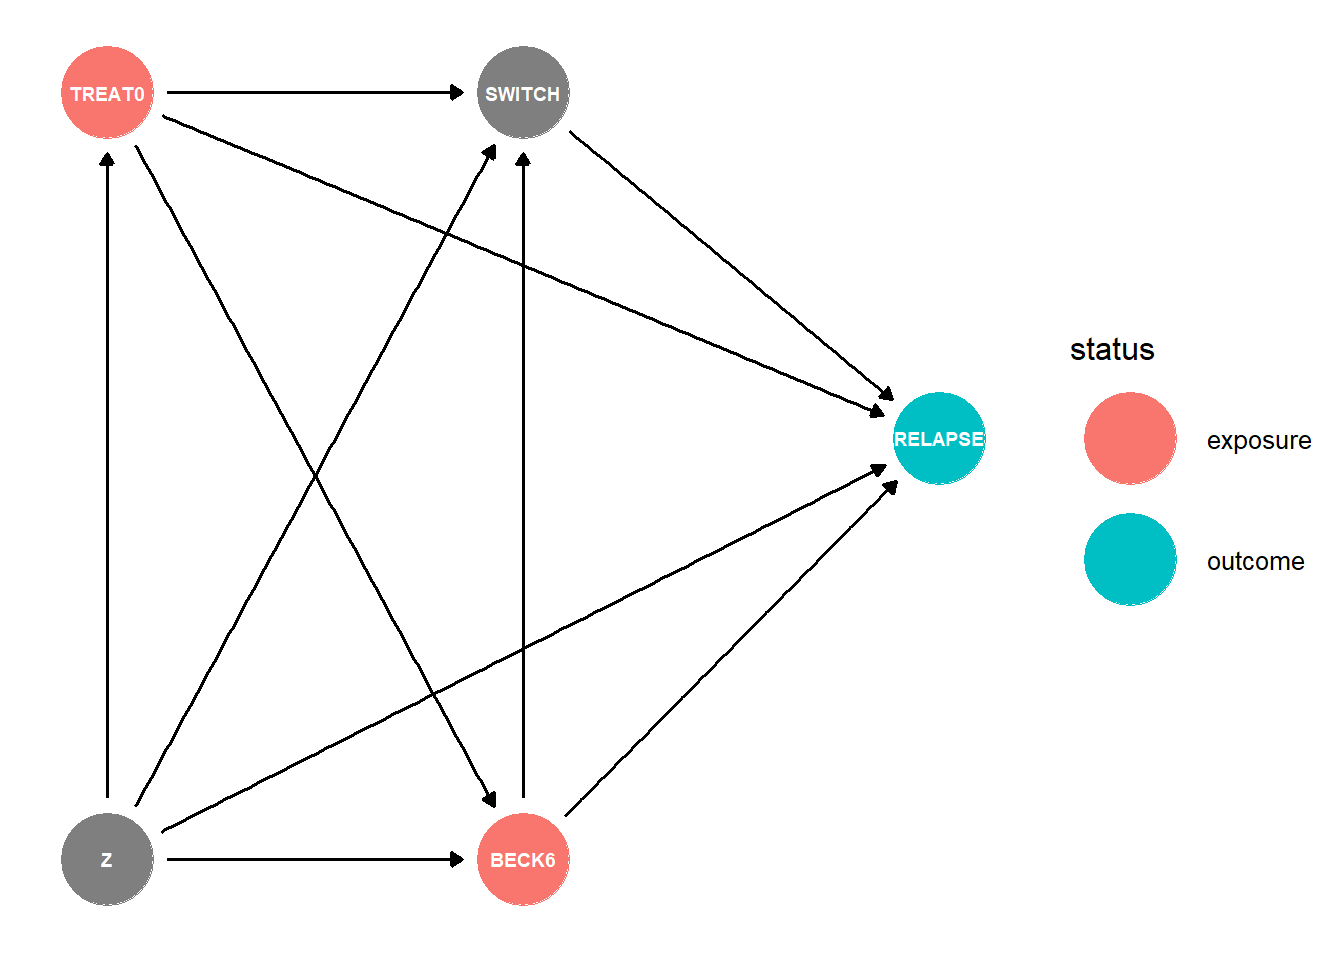
\includegraphics{_main_files/figure-latex/dag-1.pdf}

For simplicity, Z represents the confounders measured at baseline, which
include age, gender, socioeconomic status, and the Beck score.

\chapter{Causal inference estimand}\label{causal}

A causal estimand is a description of the quantity that is to be
estimated. In the context of RWD, methods such as matching or weighting
imply the selection of an estimand. Among these, two estimands are
typically of interest: the average treatment effect in the treated (ATT)
and the average treatment effect in the population (ATE).

The ATT is considered when assessing the effect of a treatment among
individuals who are likely to receive it (e.g., when comparing a new
drug to a placebo or standard of care). In our example, the research
question would be framed as: what is the treatment effect among patients
likely to receive Duloxyn? This includes individuals with
characteristics similar to those receiving Sertralex, while individuals
with characteristics unique to Duloxyn would be excluded from the
analysis. This estimator typically involves pair matching statistical
methods (\citeproc{ref-greifer_choosing_2023}{Greifer and Stuart 2023};
\citeproc{ref-heiss_demystifying_nodate}{Heiss n.d.}).

\backmatter
\end{document}
